% Gelfand seminar notes, 1973-74: source pages P000501-P000553.
% English translation (AI-made, checked against the scans), cut page by page from the cumulative working reader A4-reader-chapters01-32-opening-first1444-separated-diplomatic-r2.
% \SourcePage{GELFAND-Pnnnnnn}{label} starts a scanned page; the second argument is the number written
% on the page, if any. Editorial notes give the page, a label and the transcriber's remark; \Unclear
% marks a doubtful reading.
\SourcePage{GELFAND-P000501}{1}
\uuline{3/\mbox{\uuline{IX}}-73.}\qquad\uline{Sem. of}
\Incomplete{GELFAND-P000501}{heading-cancelled}{The entry between “Sem.” and “Gelfand” is heavily crossed out. Its reading is unresolved.}
\end{GelfandAdjacentEvidence}
\begin{GelfandAdjacentEvidence}{GELFAND-P000501}{2}

\uline{Gelfand.}

\uuline{Plan}:

1. Derived category (Kirillov, Bernstein).

2. Ahlfors — Nevanlinna theory for many variables (and according to Grauert). (Henkin, Shabat).

3. $K$-theory (simplicial version) according to Quillen (Fuchs).
\Unclear{GELFAND-P000501}{plan-k-theory}{The faint words are provisionally read as “simplicial version”.}
\end{GelfandAdjacentEvidence}
\begin{GelfandAdjacentEvidence}{GELFAND-P000501}{3}


4. Lichtenbaum’s conjecture on the connection between the $\zeta$-fn. at integers and higher $K$-theories (Manin).

5. Weil: the ideas of «Герстенцуса».
\Unclear{GELFAND-P000501}{plan-item-five}{The Cyrillic spelling is provisionally read as «Герстенцуса».}
\end{GelfandAdjacentEvidence}
\begin{GelfandAdjacentEvidence}{GELFAND-P000501}{4}


\uline{Interlude}:
\Unclear{GELFAND-P000501}{interlude-number}{The number at the left is heavily retraced, possibly 6 or 8.}
\end{GelfandAdjacentEvidence}
\begin{GelfandAdjacentEvidence}{GELFAND-P000501}{5}

\uuline{2 problems of Serre}:

1) $k[t]$, $k$ — finite;
$SL_n(k[t])$, $n\geq 3$;
$SL_n(k[t,t^{-1}])$, $n\geq 2$

These groups have finitely many generators. Are they finitely presented? (Do there exist generators with finitely many rels. among them.).

2) Coher. group: $\forall$ subgrp. with finitely many gens. is finitely presented.
Free and nilpot. are coherent.
\Unclear{GELFAND-P000501}{coherent-groups}{The faint abbreviation reads “nilpot.”.}
\end{GelfandAdjacentEvidence}
\begin{GelfandAdjacentEvidence}{GELFAND-P000501}{6}

Fund. groups of 3-dimensional manifolds are coherent
(G. P. Scott, J. Lond. Math. Soc., (2)6 (1973), 437--440). Article.
$SL_2(\Lambda)$ is coher., where $\Lambda$ — purely imaginary elem. of a quadr. field.
\Unclear{GELFAND-P000501}{lambda-description}{The faint entry is provisionally read as “purely imaginary elem. of a quadr. field”.}
\end{GelfandAdjacentEvidence}
\begin{GelfandAdjacentEvidence}{GELFAND-P000501}{7}

\Unclear{GELFAND-P000501}{lambda-cancelled}{The crossed-out word is provisionally read as “also”.}
\end{GelfandAdjacentEvidence}
\begin{GelfandAdjacentEvidence}{GELFAND-P000501}{8}


Are $SL_3(\mathbb Z)$ or $SL_2(\mathbb Z[\frac1p])$ coherent?
$GL_n(\mathbb Q)$?

[are there many rels. among distinct irreducibles? (a fin. number)]
\Unclear{GELFAND-P000501}{interlude-relations}{The faint abbreviation is provisionally read as “rels.”.}
\end{GelfandAdjacentEvidence}
\begin{GelfandAdjacentEvidence}{GELFAND-P000501}{9}

\Unclear{GELFAND-P000501}{interlude-question}{The word is provisionally read as “irreducibles”.}
\end{GelfandAdjacentEvidence}
\begin{GelfandAdjacentEvidence}{GELFAND-P000501}{10}


[Which fund. groups occur?]

6. \uline{Smale}: optimization of several functions.
\Unclear{GELFAND-P000501}{plan-six-overwriting}{The digit is heavily retraced. Its outlines and the adjacent numbering support 6.}
\end{GelfandAdjacentEvidence}
\begin{GelfandAdjacentEvidence}{GELFAND-P000501}{11}


7. \uline{Brown, Douglas, Fillmore} \quad Proper $K$-theory of several variables (Kirillov).

8. \uuline{Mishchenko}: representations in his sense.

9. \uline{Lusztig}: higher sign. of Novikov\qquad J. Diff. Geom. 197(1)
\Unclear{GELFAND-P000501}{novikov-name}{The faint name is provisionally read as “Lusztig”.}
\end{GelfandAdjacentEvidence}
\begin{GelfandAdjacentEvidence}{GELFAND-P000501}{12}


10. \uline{Atiyah, Bott, Patodi on \mbox{$L$}-functions associated with eqs.}
(spectral asymmetry, etc.) (Shubin)

11. \uuline{Donovan, Freilich} a (V. Ponomarev) — a quadruple of subspaces, etc.
\Unclear{GELFAND-P000501}{plan-item-eleven-mark}{The small mark is provisionally read as «а».}
\end{GelfandAdjacentEvidence}
\begin{GelfandAdjacentEvidence}{GELFAND-P000501}{13}

Modules, etc.

12. Yu. I. Manin.

13. Vershik, Gelfand, Graev — 6 variations on $SL_2$.

\uuline{Yu. I. Manin.}\qquad\uline{\mbox{$p$}-adic measures}

\uline{Setting}: $\mathbb Q_p$;\quad $K$ — a fin. ext.
$X$ — a compact $p$-adic analytic set over $K$.
Example: integers in $K$, their direct prod., etc.

\SourceFigure{GELFAND-P000501}{field-tower-and-maps}{The field tower at the left has no arrows. Beside it are an analytic map and an example of a coordinate.\par\smallskip
{\centering
\begingroup\color{black}\GelfandFitDiagram{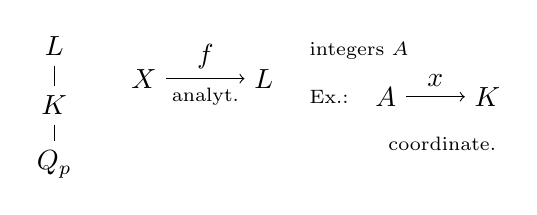
\begin{tikzpicture}
\node (L) at (0,1.50) {$L$};
\node (K) at (0,.75) {$K$};
\node (Q) at (0,0) {$\mathbb Q_p$};
\draw (L)--(K)--(Q);
\node (X) at (1.14,1.09) {$X$};
\node (cod) at (2.66,1.09) {$L$};
\draw[->] (X)--node[above] {$f$} node[below,font=\scriptsize] {analyt.} (cod);
\node[anchor=west,font=\scriptsize] at (3.12,1.45) {integers $A$};
\node[anchor=west,font=\scriptsize] at (3.12,.86) {\uline{Ex.}:};
\node (A) at (4.21,.86) {$A$};
\node (Ktwo) at (5.50,.86) {$K$};
\draw[->] (A)--node[above] {$x$} (Ktwo);
\node[anchor=west,font=\scriptsize] at (4.12,.26) {coordinate.};
\end{tikzpicture}}\endgroup\par}}
\end{GelfandAdjacentEvidence}
\begin{GelfandAdjacentEvidence}{GELFAND-P000501}{14}


\uline{Problem}: define $\int f\,d\mu$, i.e. determine a reasonable
and inter. class of measures of $p$-adic type on $X$.
\Unclear{GELFAND-P000501}{last-line-class}{The abbreviation is provisionally read as “inter.”.}
\end{GelfandAdjacentEvidence}



\Needspace{7\baselineskip}
\begin{GelfandAdjacentEvidence}{GELFAND-P000502}{1}
\SourcePage{GELFAND-P000502}{unlabelled}
\uline{Motivation}: a) there are $\zeta$-fns.
$L(s)\qquad \mathbb C\longrightarrow\mathbb C$
\[
\sum n^{-s};\qquad \sum\chi(n)n^{-s};\qquad \sum a_n n^{-s},
\]
where $\sum a_n e^{2\pi i\lambda}$ is an autom. form.
\Unclear{GELFAND-P000502}{exponential-index}{The last sign in the exponent is provisionally set as $\lambda$.}
\end{GelfandAdjacentEvidence}
\begin{GelfandAdjacentEvidence}{GELFAND-P000502}{2}


For them, a class of int. formulas with adelic integration
\[
L(\chi)=\int_{G_A/G_K}\chi\,d\mu
\]
\Unclear{GELFAND-P000502}{adele-quotient}{The denominator is provisionally set as $G_K$. There is an additional loop at the base of $G$.}
\end{GelfandAdjacentEvidence}
\begin{GelfandAdjacentEvidence}{GELFAND-P000502}{3}

\begin{flushright}
$G_K$ — princ. adeles
\end{flushright}
\Unclear{GELFAND-P000502}{adele-group-note}{The faint note is provisionally read as “$G_K$ — princ. adeles”.}
\end{GelfandAdjacentEvidence}
\begin{GelfandAdjacentEvidence}{GELFAND-P000502}{4}


In fact, the argument is a character $L(\chi)$

b) there are $p$-adic analogues of $L(\chi)$ and $\zeta(s)$
(Leopoldt — \sout{Iwasawa}\raisebox{.8ex}{\scriptsize Kubota}).
\Unclear{GELFAND-P000502}{cancelled-iwasawa}{“Iwasawa” is crossed out. “Kubota” is inserted above.}
\end{GelfandAdjacentEvidence}
\begin{GelfandAdjacentEvidence}{GELFAND-P000502}{5}

\begin{align*}
\zeta(2m)&=B_{2m}\frac{\pi^{2m}}{\ldots}\\
\zeta(1-2m)&=\,?\,\frac{B_{2m}}{2m},
\end{align*}
\[
\Vert\quad \biggl(\text{G.}\ \sum_{n=1}^{\infty}n^3=\frac{B_4}{4}
\]
\Unclear{GELFAND-P000502}{sum-intro}{The letter after the parenthesis is provisionally read as «Г.». A hatched stroke is at the left.}
\end{GelfandAdjacentEvidence}
\begin{GelfandAdjacentEvidence}{GELFAND-P000502}{6}

\Unclear{GELFAND-P000502}{bernoulli-formulas}{There are faint marks below the line between the equals sign and $\frac{B_4}{4}$. Their reading is unresolved.}
\end{GelfandAdjacentEvidence}
\begin{GelfandAdjacentEvidence}{GELFAND-P000502}{7}


even and odd differ:
\[
-y''+p(x)y=\lambda y,\qquad \sum\lambda_n^k
\]
integers and half-integers differ)

Still unknown why such a $\sum n^3$ is expr. through $B$ .)

The point of the next plan — pres. of Kronecker’s formulas.
\Unclear{GELFAND-P000502}{kronecker-abbreviation}{The abbreviation before “formulas” is provisionally read as «пред.».}
\end{GelfandAdjacentEvidence}
\begin{GelfandAdjacentEvidence}{GELFAND-P000502}{8}

Choose $p$ from the Euler prod.
\[
1-2m\longrightarrow\frac{B_{2m}}{2m}(1-p^{2m-1})
\qquad\text{Fix }p!
\]
$p$-adic cont. and even analytic !!!
\sout{(from the Euler prod. we removed the chosen \mbox{$p$})}.
\par\smallskip\hrule\smallskip
\Unclear{GELFAND-P000502}{analytic-ending}{The ending of the last word is provisionally read as «аналитичне».}
\end{GelfandAdjacentEvidence}
\begin{GelfandAdjacentEvidence}{GELFAND-P000502}{9}

\Unclear{GELFAND-P000502}{cancelled-euler-comment}{The crossed-out entry is provisionally reconstructed. A long stroke runs below the line in the manuscript.}
\end{GelfandAdjacentEvidence}
\begin{GelfandAdjacentEvidence}{GELFAND-P000502}{10}


\[
\begin{gathered}
\zeta(s)(1-p^{-s})\\
\mathbb C\longrightarrow\mathbb C
\end{gathered}
\qquad\text{between.}\qquad
\begin{gathered}
\zeta^{(p)}(s_p)\\
\mathbb Z_p\longrightarrow\mathbb Q_p
\end{gathered}
\]
\Unclear{GELFAND-P000502}{interpolation-connector}{The faint word between the two displays is provisionally read as “between”.}
\end{GelfandAdjacentEvidence}
\begin{GelfandAdjacentEvidence}{GELFAND-P000502}{11}

there is an intersection of $\mathbb C$ and $\mathbb Z_p$ (integers), the values there are the same.

\SourceFigure{GELFAND-P000502}{embedding-diagram}{The lower left letter is provisionally set as $\mathbb C$. A short arrow leads upward from it. The right arrow goes up and to the right.\par\smallskip
{\centering
\begingroup\color{black}\GelfandFitDiagram{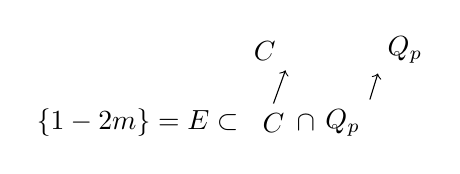
\begin{tikzpicture}
\node[anchor=east] at (0,0) {$\{1-2m\}=E\subset$};
\node (first) at (.32,0) {$\mathbb C$};
\node at (.73,0) {$\cap$};
\node (second) at (1.20,0) {$\mathbb Q_p$};
\node (c) at (.21,.91) {$\mathbb C$};
\node (q) at (1.99,.92) {$\mathbb Q_p$};
\draw[->] (first.north)--(c.south east);
\draw[->] (second.north east)--(q.south west);
\end{tikzpicture}}\endgroup\par}}
\end{GelfandAdjacentEvidence}
\begin{GelfandAdjacentEvidence}{GELFAND-P000502}{12}

and they are analytic

In fact, the correct argument is apparently adelic.
\[
\mathbb Q_p\longrightarrow\mathbb Q_{\ell}\quad(p\ne\ell)\quad
\text{apparently simpler (but unknown)}
\]
Difficult $\mathbb Q_p\longrightarrow\mathbb Q_p$,

Was begun by \uuline{Mazur}.

\uline{Measures on compact \mbox{$p$}-adic spaces.}

$K$ — fin. ext. of $\mathbb Q_p$;\quad
$A$ — integers in $K$;\quad
$A\supset\overline m$ (max. ideal)

\hfill (roots of eqs. with integral coeffs.)
\[
\operatorname{Card}(A/\overline m)\underset{\mathrm{def}}{=}q.
\]
Compact anal. set over $K$.
\[
A^n=\underbrace{A\times\ldots\times A}_{n}
\quad\text{— $n$-dimensional ball}
\]
\uline{Anal. set}: space and a sheaf of fns., loc. structure — a ball.

\uline{Theorem} (Serre): $X$ — a comp. an. set over $K$ of dim. $n$. Then

a) $X\simeq rA^n$ (analytic isom.), $r\in\mathbb N$
\Unclear{GELFAND-P000502}{theorem-count}{The number of balls is provisionally set as $r$, possibly $\tau$.}
\end{GelfandAdjacentEvidence}
\begin{GelfandAdjacentEvidence}{GELFAND-P000502}{13}


\SourceFigure{GELFAND-P000502}{serre-disjoint-balls}{Four ovals with a label at the right.\par\smallskip
{\centering
\begingroup\color{black}\GelfandFitDiagram{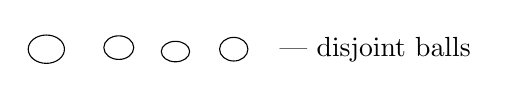
\begin{tikzpicture}
\draw (0,0) ellipse (.23 and .18);
\draw (.92,.02) ellipse (.19 and .15);
\draw (1.64,-.03) ellipse (.18 and .13);
\draw (2.38,0) ellipse (.18 and .15);
\node[anchor=west] at (2.84,0) {— disjoint balls};
\end{tikzpicture}}\endgroup\par}}
\end{GelfandAdjacentEvidence}
\begin{GelfandAdjacentEvidence}{GELFAND-P000502}{14}


b) \sout{if}
\[
rA^n\simeq r'A^n\quad
\mathrel{\tikz[baseline=(equiv.base)]\node[draw,ellipse,inner sep=1pt] (equiv) {$\Leftrightarrow$};}
\quad r\equiv r'\ \operatorname{mod}(q-1)
\]
\Unclear{GELFAND-P000502}{serre-cancelled-condition}{The crossed-out word is provisionally read as “if”. The equivalence sign is encircled.}
\end{GelfandAdjacentEvidence}



\Needspace{7\baselineskip}
\begin{GelfandAdjacentEvidence}{GELFAND-P000503}{1}
\SourcePage{GELFAND-P000503}{2}
\[
A=\{a\in K\mid a\text{ is integral}\}.\qquad
A=\bigcup_{a_i\ \mathrm{mod}\ m}\{a\equiv a_i\ \mathrm{mod}\ m\}.
\]
\uwave{How to compute \mbox{$r$}?}
\Unclear{GELFAND-P000503}{invariant-letter}{The letter is provisionally set as $r$.}
\end{GelfandAdjacentEvidence}
\begin{GelfandAdjacentEvidence}{GELFAND-P000503}{2}


\uline{Examples}: a) $X$ — an alg. set over $A$
(a smooth scheme over $\operatorname{Spec}A$).

\sout{How to compute \mbox{$r$} from pt. a) of Serre’s theor.?}
\Unclear{GELFAND-P000503}{cancelled-question}{The crossed-out question is read provisionally. The strokes over the part number are particularly heavy.}
\end{GelfandAdjacentEvidence}
\begin{GelfandAdjacentEvidence}{GELFAND-P000503}{3}


Reduction $X_0\quad
\underset{\text{over }\operatorname{Spec}A.}{\text{(closed fibre)}}$
— an alg. set over $A/\bar m$
\[
\operatorname{Card}X_0(A/\bar m)=r(X).
\]
\uwave{Example} of a scheme: $X=P^1$ or a circle.
\quad 2 aff. lines glued by $x=y^{-1}$

Reduction: proj. line over a fin. field of $q$ elems. — there are $q+1$ elems.
\[
q+1=2\ \mathrm{mod}(q-1).
\]
So 2 balls:
\SourceFigure{GELFAND-P000503}{two-balls}{The top of the left contour is blacked out. The arrows of the right contour point towards its upper gap. At the right are “and” and a small round sign.\par\smallskip
{\centering
\begingroup\color{black}\GelfandFitDiagram{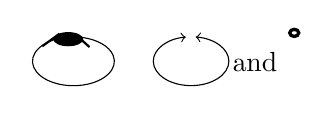
\begin{tikzpicture}
\draw (-.12,.31) arc[start angle=104,end angle=438,x radius=.52,y radius=.31];
\fill (-.06,.29) ellipse (.19 and .09);
\draw[line width=.8pt] (-.39,.20)--(-.17,.36) (.02,.36)--(.21,.19);
\draw[->] (1.50,-.30) arc[start angle=270,end angle=443,x radius=.48,y radius=.31];
\draw[->] (1.50,-.30) arc[start angle=270,end angle=98,x radius=.48,y radius=.31];
\node at (2.31,.00) {and};
\draw[very thick] (2.81,.37) ellipse (.057 and .045);
\end{tikzpicture}}\endgroup\par}}
\end{GelfandAdjacentEvidence}
\begin{GelfandAdjacentEvidence}{GELFAND-P000503}{4}

\[
P^1(K)=\mathbb Q_p\cup\infty,\qquad pA\cup A^{-1}.
\]

b) $X$ — $p$-adic comp. Lie grp.; it is profinite, $\forall$ factor has an order.

Order: $2^2\,3^\infty\,5^1\,7^0\,11^\infty\ldots$ —
a supernatural number (since they divide one another).
\SourceFigure{GELFAND-P000503}{supernatural-exponent}{The stroke left of the exponent belongs to the digit $5$. The exponent reads $1$.}
\end{GelfandAdjacentEvidence}
\begin{GelfandAdjacentEvidence}{GELFAND-P000503}{5}


It turns out $\operatorname{ord}X=p^\infty\cdot N$,
where $(p,N)=1$, $N$ — an ord. integer.
\[
\underline{\underline{N=r(X)}}
\]
$SL_2$ — $(p-1)$ balls $(=p^2-1\ \mathrm{mod}\ p)$
\SourceFigure{GELFAND-P000503}{sl2-count}{The manuscript reads $p^2-1\ \mathrm{mod}\ p$.}
\end{GelfandAdjacentEvidence}
\begin{GelfandAdjacentEvidence}{GELFAND-P000503}{6}


\SourceFigure{GELFAND-P000503}{margin-fields}{The mark between $L$ and $K$ is blacked out. Its shape and direction are unresolved.\par\smallskip
{\centering
\begingroup\color{black}\GelfandFitDiagram{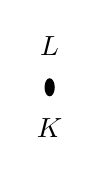
\begin{tikzpicture}
\node at (0,.52) {$L$};
\fill (0,0) ellipse (.065 and .115);
\node at (0,-.52) {$K$};
\end{tikzpicture}}\endgroup\par}}
\end{GelfandAdjacentEvidence}
\begin{GelfandAdjacentEvidence}{GELFAND-P000503}{7}

\uline{Definition}: $L$-measure on $X$ — an $L$-valued finitely addit. fn. on open-and-closed subsets of $X$.

($X$ — a comp. anal. set).
\Unclear{GELFAND-P000503}{definition-overwrite}{The start of “anal.” is heavily overwritten.}
\end{GelfandAdjacentEvidence}
\begin{GelfandAdjacentEvidence}{GELFAND-P000503}{8}


\uline{Examples}: a) $X=\mathbb Z_p$
\SourceFigure{GELFAND-P000503}{clopen-tree}{Four branches descend from the vertex $X$. Some lower strokes merge.\par\smallskip
{\centering
\begingroup\color{black}\GelfandFitDiagram{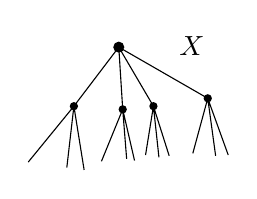
\begin{tikzpicture}
\coordinate (root) at (0,1.65);
\coordinate (a) at (-.57,.90);
\coordinate (b) at (.05,.86);
\coordinate (c) at (.44,.90);
\coordinate (d) at (1.13,1.00);
\draw (root)--(a) (root)--(b) (root)--(c) (root)--(d);
\draw (a)--(-1.15,.19) (a)--(-.66,.12) (a)--(-.44,.09);
\draw (b)--(-.22,.20) (b)--(.10,.23) (b)--(.20,.21);
\draw (c)--(.34,.28) (c)--(.51,.25) (c)--(.64,.27);
\draw (d)--(.94,.30) (d)--(1.23,.27) (d)--(1.39,.28);
\fill (root) circle (2pt);
\foreach \vertex in {a,b,c,d}{\fill (\vertex) circle (1.5pt);}
\node at (.93,1.66) {$X$};
\end{tikzpicture}}\endgroup\par}}
\end{GelfandAdjacentEvidence}
\begin{GelfandAdjacentEvidence}{GELFAND-P000503}{9}


The vertices are open-and-closed subsets.

Construct these measures successively. We obtain a fund. syst. of neighbourhoods.
\[
\begin{gathered}
\text{Measure on }X\leftrightarrow
\{\mu(a+(p^m))\in L;\quad a\ \mathrm{mod}(p^m),\ m\in\mathbb N\}.\\
\mu(a+(p^m))=\sum_{b\equiv a\ \mathrm{mod}\ p^m}\mu(b+(p^{m+1}))\}
\end{gathered}
\]
\SourceFigure{GELFAND-P000503}{measure-braces}{Each of the two written lines ends in a closing brace.}
\end{GelfandAdjacentEvidence}
\begin{GelfandAdjacentEvidence}{GELFAND-P000503}{10}


And this applies to any compact subset.

\[
\text{b) }\mu(a+(p^m))=\underbrace{\mathrm{const}\cdot p^{-m}}_{\in L}
\quad\text{— \uuline{invar. measures.}}
\]
There is on $L$ a metric ($p$-adic absolute value).
\[
|\mathrm{const}\cdot p^{-m}|_L\longrightarrow\infty\quad
\text{as }m\longrightarrow\infty.
\]
The smaller the sets, the larger the measure!!

It cannot tend to zero! It would follow from the non-Archim. property that the measure of the whole equals $0$.

Invar. measures are bad.

The slowest-growing is bounded.
\[
\text{c) }\mu(a+(p^m))=1\text{ if }a<\frac{p^m}{2},\qquad
-1\text{ if }a>p^m/2
\]
\SourceFigure{GELFAND-P000503}{measure-signs}{The left value is $1$ and the right value is $-1$. The first threshold uses a stacked fraction and the second a slash.}
\end{GelfandAdjacentEvidence}
\begin{GelfandAdjacentEvidence}{GELFAND-P000503}{11}

\begin{flushright}
$\Vert$ nontriv. bounded measure
\end{flushright}
$0<a<p^m$,\quad $(a,p)=1$ \quad Measure on $\mathbb Z_p^*$.
\Incomplete{GELFAND-P000503}{bottom-cancelled-glyph}{A short entry between $0<a<p^m$ and $(a,p)=1$ is crossed out. Its reading is unresolved.}
\end{GelfandAdjacentEvidence}



\Needspace{7\baselineskip}
\begin{GelfandAdjacentEvidence}{GELFAND-P000504}{1}
\SourcePage{GELFAND-P000504}{unlabelled}
\uline{Exercise}: check additivity. Interference occurs.

Integr. against it — $\zeta$-fns. of Leopoldt — Kubota.

Mazur devised this measure.

\uline{Integrals.}\qquad
$X$, $\mu$ — a measure with vals. in $L$.
\SourceFigure{GELFAND-P000504}{field-map-L-to-K}{In the right margin an arrow points down from $L$ to $K$.\par\smallskip
{\centering
\begingroup\color{black}\GelfandFitDiagram{\begin{tikzpicture}
\node (L) at (0,.86) {$L$};
\node (K) at (0,0) {$K$.};
\draw[->] (L)--(K);
\end{tikzpicture}}\endgroup\par}}
\end{GelfandAdjacentEvidence}
\begin{GelfandAdjacentEvidence}{GELFAND-P000504}{2}


$X\overset f\longrightarrow L$, analyt. fn.
\[
\int_X f\,d\mu
\]
\[
R=\{(U_i),\quad\underset{\text{open-and-closed}}{U_i}
\text{ — a partition of }X,\quad a_i\in U_i\}
\]
\[
S(f,R)=\sum f(a_i)\mu(U_i).
\]
\[
\int_X f\,d\mu=\lim_R S(f;R)
\]
if the limit exists under refinement

\uline{Example.}\qquad $X=\mathbb Z_p$, $\mu$ — invar.
\(\bigl(\mu(a+(p^m))=p^{-m}.\bigr)\),

$L=\mathbb Q_p$.\qquad $f=1$ is integrable

\uuline{\mbox{$f=x$}} — simple nonconst.
\[
\int f\,d\mu\quad\text{does not exist!}
\]
\[
R=\{0\le a\le p^m-1,\quad a\in U_a\equiv\{b\mid b\equiv a\ \mathrm{mod}\ p^m\}.
\]
\Unclear{GELFAND-P000504}{partition-exponent-cancelled}{An entry resembling $-1$ is crossed out after the exponent $m$. The next $-1$ is part of the bound itself.}
\end{GelfandAdjacentEvidence}
\begin{GelfandAdjacentEvidence}{GELFAND-P000504}{3}

\[
S(f,R)=\frac1{p^m}\underbrace{\sum_{a=0}^{p^m-1}a}_{\displaystyle\frac{(p^m-1)p^m}{2}}
\longrightarrow-\frac12
\]
\Unclear{GELFAND-P000504}{sum-exponent-cancelled}{Below the brace, an entry resembling $-1$ is crossed out after the exponent $m$ of the first $p$.}
\end{GelfandAdjacentEvidence}
\begin{GelfandAdjacentEvidence}{GELFAND-P000504}{4}


But this is not the only limit point.
\[
R'=\{p^m\in U_0\quad\text{the rest as in }R\}
\]
\uline{The limit will be different}: variation of the fn. on the interval $\approx$ measure of the interv.

\uline{hence a cond. on the measure}: under refinement the ratio of the measure to the invar. measure must $\longrightarrow0$ (this is in the case $n=1$).

\uline{Theorem}: let $X$ be one-dimensional over $\mathbb Q_p$

1) $\mu$ — a measure on $X$ with vals. in $L$, moderately growing,
i.e.
\[
U\longrightarrow\underset{\text{point}}{\bullet}
\Longrightarrow
\left|\frac{\mu(U)}{\mu_{\mathrm{inv}}(U)}\right|_L\longrightarrow0
\]
\Unclear{GELFAND-P000504}{moderate-overwrite}{The beginning of “moderately” is heavily retraced.}
\end{GelfandAdjacentEvidence}

($\mu_{\mathrm{inv}}$ — the usual inv. meas. on $\mathbb Z_p$).

2) $f:X\longrightarrow L$ satisfies the Lipschitz cond. with exponent $1$

Then $\int f\,d\mu$ exists.

\begin{flushright}
$\Vert$ \uwave{Next time}: concrete measures and mod. forms.
\end{flushright}


\Needspace{7\baselineskip}
\begin{GelfandAdjacentEvidence}{GELFAND-P000505}{1}
\SourcePage{GELFAND-P000505}{unlabelled}
\Unclear{GELFAND-P000505}{top-right-label}{The entry beyond the right border is cut off by the edge of the scan. Its reading is unresolved.}
\end{GelfandAdjacentEvidence}
\begin{GelfandAdjacentEvidence}{GELFAND-P000505}{2}


\uwave{10.9.73.}\qquad\uuline{Gelfand Sem.}

\uuline{Manin}\quad(\uwave{continued}).

$X$ — 1-dimensional $p$-adic space;

$\mu$ — $K$-measure on $X$\qquad
($K$ — a fin. ext. of $\mathbb Q_p$)

\underline{$f:X\longrightarrow K$}

\[
R:\quad\text{Riemann data: }\{X=\bigcup_{i=1}^n U_i\,
\text{\sout{\}}},\quad a_i\in U_i\}.
\]
\Unclear{GELFAND-P000505}{riemann-cancelled-brace}{A crossed-out closing brace is visible after $U_i$.}
\end{GelfandAdjacentEvidence}
\begin{GelfandAdjacentEvidence}{GELFAND-P000505}{3}

\[
S(f,R)=\sum\mu(U_i)f(a_i).
\]

\uline{Theorem}:

$\exists\int_X f\,d\mu$, if

a) $f$ is Lipschitz with exp. $1$

b) $(U\mapsto\text{point})\Longrightarrow
\left|\mu(U)/\mu_{\mathrm{inv}}(U)\right|\longrightarrow0$.

\uuline{Example.}\qquad $X=\mathbb Z_p$;
\[
\mu(a+(p^m))=
\begin{cases}
-1&\text{if }0\le a<\dfrac{p^m}{2}\\
+1&\text{if }\dfrac{p^m}{2}<a<p^m.
\end{cases}
\]
\uwave{Tree of open-and-closed subsets}:
\SourceFigure{GELFAND-P000505}{clopen-moment-tree}{Three strokes extend upward from the top circle. There are two three-ray forks below. A 1 is written at the upper branch.\par\smallskip
{\centering
\begingroup\color{black}\GelfandFitDiagram{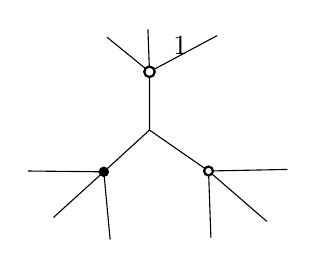
\begin{tikzpicture}
\coordinate (top) at (0,1.66);
\coordinate (fork) at (0,.92);
\coordinate (left) at (-.58,.39);
\coordinate (right) at (.75,.40);
\draw (top)--(-.54,2.10) (top)--(-.02,2.20) (top)--(.86,2.12);
\draw (top)--(fork) (fork)--(left) (fork)--(right);
\draw (left)--(-1.54,.40) (left)--(-1.22,-.19) (left)--(-.50,-.47);
\draw (right)--(1.75,.42) (right)--(1.49,-.24) (right)--(.78,-.45);
\filldraw[fill=white,thick] (top) circle (1.9pt) (right) circle (1.6pt);
\fill (left) circle (1.9pt);
\node at (.39,1.99) {$1$};
\end{tikzpicture}}\endgroup\par}}
\end{GelfandAdjacentEvidence}
\begin{GelfandAdjacentEvidence}{GELFAND-P000505}{4}


$f(x)=x^{2r-1}$\qquad (for $f(x)=x^{2r}$ one gets 0).
\Unclear{GELFAND-P000505}{moment-index}{The letter resembles $\tau$ and is provisionally set as $r$.}
\end{GelfandAdjacentEvidence}
\begin{GelfandAdjacentEvidence}{GELFAND-P000505}{5}


\[
\int_{\mathbb Z_p}x^{2r-1}\,d\mu=(-1)^r(1-2^{-r})\frac{B_{r-1}}{2r}
\]
\[
\mathbb Z_p=\bigcup_{0\le a<p^{m-1}}\{a+p^m\mathbb Z_p\}.
\]
\SourceFigure{GELFAND-P000505}{union-upper-bound}{In the upper bound, $-1$ is written at the level of the exponent $m$.}
\end{GelfandAdjacentEvidence}
\begin{GelfandAdjacentEvidence}{GELFAND-P000505}{6}


$R$
\Unclear{GELFAND-P000505}{margin-r}{The sign in the left margin is heavily retraced. Provisionally read as $R$.}
\end{GelfandAdjacentEvidence}
\begin{GelfandAdjacentEvidence}{GELFAND-P000505}{7}

\[
S(f,R)=-\sum_{0\le a<p^m/2}a^{2r-1}
+\sum_{p^m>a>p^m/2}a^{2r-1}
\]

There are Voronoi formulas interpreted as evaluations of integrals of this kind.

\[
\int_{\mathbb Z_p^*}=\int_{\mathbb Z_p}-\int_{p\mathbb Z_p}
\]
\[
\begin{aligned}
\int_{\mathbb Z_p^*}x^{2r-1}\,d\mu
&=(1-p^{2m-1})\int_{\mathbb Z^p}\\
&=(-1)^r(1-p^{2m-1})\cdot(1-2^{-r})\frac{B_{r-1}}{2r}=
\end{aligned}
\]
\SourceFigure{GELFAND-P000505}{lower-powers}{The exponent is written as $2m-1$ in both factors.}
\end{GelfandAdjacentEvidence}
\begin{GelfandAdjacentEvidence}{GELFAND-P000505}{8}

\SourceFigure{GELFAND-P000505}{lower-integral-domain}{The $p$ is written to the upper right of $\mathbb Z$.}
\end{GelfandAdjacentEvidence}


(computed by the Mellin transf. of characters)
\[
=(\ldots)\zeta_{(p)}(1-2r)
\]


\Needspace{7\baselineskip}
\begin{GelfandAdjacentEvidence}{GELFAND-P000506}{1}
\SourcePage{GELFAND-P000506}{5}
Consider $X=\operatorname{Hom}(\mathbb Z_p^*;K^*)$.
\Unclear{GELFAND-P000506}{hom-codomain}{The mark above $K$ merges with the parenthesis. Provisionally read as a star.}
\end{GelfandAdjacentEvidence}
\begin{GelfandAdjacentEvidence}{GELFAND-P000506}{2}

\[
\mathbb Z_p^*=(\mathbb Z/p\mathbb Z)^*\times(1+p)^{\mathbb Z_p}.
\]
$\chi\in X\Longrightarrow\chi=\chi_0\cdot\chi_1$, where
\[
\begingroup\color{black}\GelfandFitDiagram{\begin{tikzpicture}[baseline=(conditions.base)]
\node[inner sep=2pt] (conditions) {$\begin{aligned}
\chi_0&=1\quad\text{on }(1+p)^{\mathbb Z_p}.\\
\chi_1&=1\quad\text{on }(\mathbb Z/p\mathbb Z)^*.
\end{aligned}$};
\draw ([xshift=-2pt,yshift=7pt]conditions.south west)
  |- ([xshift=4pt]conditions.south east);
\end{tikzpicture}}\endgroup
\]
\[
\forall u\in\mathbb Z_p^*: \quad u=\varepsilon\cdot(1+p)^a,\qquad
\text{where }\varepsilon^{p-1}=1,\quad a\in\mathbb Z_p
\]

Therefore
\SourceFigure{GELFAND-P000506}{character-product}{%
\begingroup\color{black}\GelfandFitDiagram{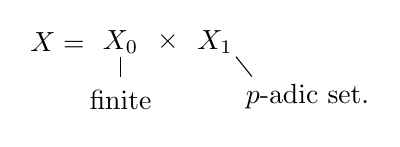
\begin{tikzpicture}
\node[inner sep=1pt] at (0,0) {$X=$};
\node[inner sep=1pt] (finite) at (.8,0) {$X_0$};
\node[inner sep=1pt] at (1.4,0) {$\times$};
\node[inner sep=1pt] (adic) at (2,0) {$X_1$};
\draw (finite.south) -- ++(0,-.25);
\draw (adic.south east) -- ++(.20,-.25);
\node[anchor=north] at (.8,-.49) {finite};
\node[anchor=north west,inner sep=1pt] at (2.35,-.49) {$p$-adic set.};
\end{tikzpicture}}\endgroup}
\end{GelfandAdjacentEvidence}
\begin{GelfandAdjacentEvidence}{GELFAND-P000506}{3}


\hfill Thus: $X$ — $p$-adic set\par

\[
\chi_1(1+p)=1+t,\qquad t\in\overline{m}.\qquad
\text{(notation: }\chi_{(t)}\text{)}
\]
Hence $X_1\cong\overline{m}$ (but with a different law of composition)
\SourceFigure{GELFAND-P000506}{composition-retrace}{The first letter of the Russian word for “but” is heavily retraced.}
\end{GelfandAdjacentEvidence}
\begin{GelfandAdjacentEvidence}{GELFAND-P000506}{4}


\uline{Theorem}. If $\mu$ grows moderately (more slowly than an invari. one), then
\[
\int_{\mathbb Z_p^*}\chi\,d\mu\quad\text{is analytic in $\chi$}.
\]

\uline{In more detail}:
\[
\int\chi_{(t)}\,d\mu=F(t)\in K[[t]]
\]
converges for $|t|<1$.

Next: $\int x^s\,d\mu$ is analytic in $s$ for $s\equiv0\ (\operatorname{mod}(p-1))$
and for $s=k\operatorname{mod}(p-1)$
\SourceFigure{GELFAND-P000506}{power-integrand}{The integrand reads $x^s$.}
\end{GelfandAdjacentEvidence}
\begin{GelfandAdjacentEvidence}{GELFAND-P000506}{5}


\begin{center}— · —\end{center}
\uline{Modular forms}. $\Gamma=SL(2,\mathbb Z)/(\pm1)$ acts on
\[
H=\{z\in\mathbb C\mid\operatorname{Im}z>0\},\qquad w\equiv0\ (2),\qquad w\geq0
\]
$\underline{P}_w$: \uwave{Parab. forms of weight \mbox{$w+2$} on \mbox{$H$}:}

a) $\varphi(z)(dz)^{\frac{w+2}{2}}$ $\Gamma$-invariant

b) $\varphi(z)=\displaystyle\sum_{n=1}^\infty a_ne^{2\pi inz}$

1st nontriv. fn. at $w+2=12$ with gaps up to $26$
(1-dimensional), then a fin.-dim. space throughout
[Crossed out: \Incomplete{GELFAND-P000506}{modular-cancellation}{The reading under the heavy strikeout is unresolved.}
\end{GelfandAdjacentEvidence}
]
\[
w+2=12\quad\Longrightarrow\quad
e^{2\pi iz}\prod_{n=1}^\infty(1-e^{2\pi inz})^{24}
=\sum_{n=1}^\infty\tau(n)e^{2\pi inz}
\]
\begin{center}— · —\end{center}
In $P_w$ there exists a basis of forms with algebraic integer coefficients


\Needspace{7\baselineskip}
\begin{GelfandAdjacentEvidence}{GELFAND-P000507}{1}
\SourcePage{GELFAND-P000507}{unlabelled}
and such that if $\displaystyle\sum_1^\infty a_ne^{2\pi inz}$ — an elem. of this basis, then
\[
\sum a_nn^{-s}=\prod_p\frac{1}{1-a_pp^{-s}+p^{w+1-\text{[?]}}}.
\]
\Unclear{GELFAND-P000507}{euler-exponent}{The end of the exponent in the first product is overwritten. Readings: $2s$ or a sign resembling $k$.}
\end{GelfandAdjacentEvidence}
\begin{GelfandAdjacentEvidence}{GELFAND-P000507}{2}


(For each [Crossed out: $p$-adic.; above the line, circled: parab.]
form we will construct a par. measure below)
\SourceFigure{GELFAND-P000507}{form-insertion}{The circled insertion “parab.” points to the crossed-out word.}
\end{GelfandAdjacentEvidence}
\begin{GelfandAdjacentEvidence}{GELFAND-P000507}{3}


\uwave{Hecke op.}: let us see what the values of $a$, are if
\[
\sum a_nn^{-s}=
\frac{1}{\left(1-\lambda_pp^{-s}+p^{w+1-2s}\right)}
\left(\sum\ldots\right)
\]
i.e.
\[
\sum a_nn^{-s}=
\underset{\substack{\vert\\\text{known}}}{\left(\qquad\right)}
\underset{\substack{\vert\\\text{undet.}}}
  {\left(\sum b_nn^{-s}\right)}
\]
\SourceFigure{GELFAND-P000507}{factor-labels}{The empty parentheses are labelled “known” and the series “undet.”.}
\end{GelfandAdjacentEvidence}
\begin{GelfandAdjacentEvidence}{GELFAND-P000507}{4}

\[
1-\lambda p^{-s}+p^{w+1-2s}=(1-\alpha_1p^{-s})(1-\alpha_2p^{-s}).
\]
We get a lin. condition on the coeffs. $a_n$.

All together — an infin. matrix.
\Unclear{GELFAND-P000507}{matrix-afterword}{The mark after the period is heavily overwritten. Its reading is unresolved.}
\end{GelfandAdjacentEvidence}
\begin{GelfandAdjacentEvidence}{GELFAND-P000507}{5}


This cond. $\Longleftrightarrow$ The coeff. vector is an eigenvector of the Hecke operator.

Let us write its action on the fn. instead of on the Fourier coeffs.
\[
(\Phi\mid T_p)(z)\underset{\mathrm{def}}{=}
p^{w+1}\Phi(pz)+p^{-1}\sum_{k=0}^{p-1}\Phi\left(\frac{z+k}{p}\right).
\]
Eigenfns. $\Longleftrightarrow$ extract the $p$-factor from the corr. Dirichlet series.
\[
(P_w\mid T_p)=P_w.
\]

\uline{Measures: on \mbox{$\mathbb Z_p^*$}, assoc. with}
$\varphi$, $\varphi\mid T_p=\lambda_p\varphi\quad\forall p$.

[Crossed out: \Unclear{GELFAND-P000507}{measure-value-cancellation}{Possibly $\mathbb Q_p$. The reading under the strikeout is unresolved.}
\end{GelfandAdjacentEvidence}
\begin{GelfandAdjacentEvidence}{GELFAND-P000507}{6}
]
with values in $\{\mathbb Q_p(\lambda_1,\ldots,\lambda_p,\ldots)\}_p$

\uwave{Half-measures with values in}
[Crossed out: \Unclear{GELFAND-P000507}{field-cancellation}{Possibly $\mathbb Q$. The reading under the strikeout is unresolved.}
\end{GelfandAdjacentEvidence}
\begin{GelfandAdjacentEvidence}{GELFAND-P000507}{7}
]
\uwave{\mbox{$\mathbb C$}.}

$x\in\mathbb Q$.\qquad
$P(x)=\displaystyle\int_x^{i\infty}\Phi(z)\,dz$
\SourceFigure{GELFAND-P000507}{period-path}{%
\begingroup\color{black}\GelfandFitDiagram{\begin{tikzpicture}
\draw (-1.2,0) -- (1.4,0);
\draw[->] (0,1.35) -- (0,0);
\end{tikzpicture}}\endgroup}
\end{GelfandAdjacentEvidence}
\begin{GelfandAdjacentEvidence}{GELFAND-P000507}{8}


Convergence: obvious at the upper end $(e^{2\pi inz}\to0)$, and unclear at the lower end.
From the funct. eq.: it converges at the lower end too, but the dependence on $x$ is discontinuous (from subtle arithmetic).
At irr. points it generally diverges. $P(x+1)=P(x)$.

$\lambda_pP(x)=\displaystyle\int_x^{i\infty}\Phi(z)\mid T_p\,dz$
we substitute and get a funct. eq.
\[
\lambda_pP(x)=p^wP(px)+\sum_{k=0}^{p-1}P\left(\frac{x+k}{p}\right)
\]
\Unclear{GELFAND-P000507}{isolated-p}{A separate sign resembling $p$ or $P$ stands over the argument in the right-hand summand.}
\end{GelfandAdjacentEvidence}

\[
\frac{a}{p^m}\sim a+p^m\mathbb Z_p.
\]
The measure $P\left(\frac{a}{p^m}\right)$ gives almost fin. additivity.


\Needspace{7\baselineskip}
\begin{GelfandAdjacentEvidence}{GELFAND-P000508}{1}
\SourcePage{GELFAND-P000508}{6}
\uline{Correction}:
\[
\mu_\Phi(a+p^m\mathbb Z_p)=
\varrho^{-m}P\left(\frac{a}{p^m}\right)
-p^w\varrho^{-(m+m)}P\left(\frac{a}{p^{m+1}}\right)\qquad (?).
\]
\SourceFigure{GELFAND-P000508}{correction-formula}{The second exponent on $\varrho$ reads $-(m+m)$. The last denominator reads $p^{m+1}$. The $(?)$ is in the manuscript.}
\end{GelfandAdjacentEvidence}
\begin{GelfandAdjacentEvidence}{GELFAND-P000508}{2}


We get a measure on $\mathbb Z_p^*$.

\sout{Until next time}
\SourceFigure{GELFAND-P000508}{closing-cancellation}{Two strokes cross out the phrase. The last word reads “раз”.}
\end{GelfandAdjacentEvidence}


\begin{center}— · —\end{center}


\Needspace{7\baselineskip}
\begin{GelfandAdjacentEvidence}{GELFAND-P000509}{1}
\SourcePage{GELFAND-P000509}{unlabelled}
17.9.73. \quad\uline{Gelfand Sem.}
\Unclear{GELFAND-P000509}{date-day}{The second digit of the day is overwritten. A 7 is visible over the earlier strokes.}
\end{GelfandAdjacentEvidence}
\begin{GelfandAdjacentEvidence}{GELFAND-P000509}{2}


\uline{Yu. I. Manin} (continued)
\[
P(x)=\int_x^{i\infty}\Phi(z)\,dz
\]
Consider the eq. $\varrho^2-\lambda_p\varrho+p^{w+1}=0$.
and $\varrho$ is any root of it

\uline{Proposition}. Put
\[
\mu_\Phi\bigl(a+(p^{m+1})\bigr)
=\varrho^{-m}P\left(\frac{a}{p^{m+1}}\right)
-p^w\varrho^{-(m+1)}P\left(\frac{a}{p^m}\right).
\]
Then this is a half-measure (on $\mathbb Z_p^*$ taking values in $\mathbb C$ and fin.-additive).

Consider \uwave{the periods of the form}:
\[
\tau_k(\varphi)=\int_0^{i\infty}\varphi(z)z^k\,dz,\qquad 0\leq k\leq w.
\]
\[
L_\varphi(s)=\sum_{n=1}^\infty\lambda_n n^{-s}
=\frac{(2\pi)^s}{\Gamma(s)}\int_0^\infty\varphi(iy)y^{s-1}\,dy
\]
\[
\tau_k(\varphi)=\frac{k!\,i^{k+1}}{(2\pi)^{k+1}}L_\varphi(k+1)
\]
$[1,w+1]$ — crit. strip (funct. eq. relative to it)

\uline{Proposition}. $\forall x\in\mathbb Q,\ 
P(x)\in\displaystyle\sum_{k=0}^w\mathbb Z\cdot\tau_k(\Phi)$

$\operatorname{Re}$ and $\operatorname{Im}$ have a common transcend. factor. Dividing by it gives algebraic
\[
\int_{b/d}^{i\infty}\Phi(z)\,dz=\int_0^{i\infty}-\int_0^{b/d}
\]
(in neighbourhoods of points of the axis, integrate along geodesics).

\uline{Contour:}
\SourceFigure{GELFAND-P000509}{contour}{%
\begingroup\color{black}\GelfandFitDiagram{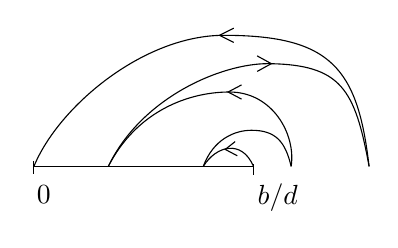
\begin{tikzpicture}[x=.90cm,y=.90cm]
\draw (0,0) -- (3.1,0);
\draw (0,-.10) -- (0,.08);
\draw (3.1,-.12) -- (3.1,.04);
\node[below] at (.14,-.13) {$0$};
\node[below right] at (3.02,-.10) {$b/d$};
\draw (0,0) .. controls (.35,.85) and (1.55,1.85) .. (2.68,1.85)
  .. controls (4.2,1.85) and (4.57,1.38) .. (4.73,0);
\draw (1.05,0) .. controls (1.52,.98) and (2.65,1.45) .. (3.30,1.45)
  .. controls (4.34,1.44) and (4.53,1.09) .. (4.73,0);
\draw (1.05,0) .. controls (1.45,.78) and (2.18,1.05) .. (2.76,1.05)
  .. controls (3.37,1.05) and (3.70,.45) .. (3.63,0);
\draw (2.39,0) .. controls (2.53,.38) and (2.83,.51) .. (3.07,.51)
  .. controls (3.42,.51) and (3.55,.34) .. (3.63,0);
\draw (2.39,0) .. controls (2.57,.29) and (2.93,.39) .. (3.10,0);
\draw (2.82,1.95) -- (2.62,1.85) -- (2.82,1.75);
\draw (3.15,1.56) -- (3.35,1.45) -- (3.15,1.34);
\draw (2.93,1.15) -- (2.74,1.05) -- (2.93,.95);
\draw (2.84,.35) -- (2.70,.24) -- (2.87,.15);
\end{tikzpicture}}\endgroup\par
\smallskip The inner arcs partly overlap. The direction of the fourth arc from the top is unresolved.}
\end{GelfandAdjacentEvidence}
\begin{GelfandAdjacentEvidence}{GELFAND-P000509}{3}


from the cont. fraction exp.
\[
\frac bd=\frac{b_m}{d_m},\quad\frac{b_{m-1}}{d_{m-1}},\quad
\ldots,\quad\frac{b_0}{d_0}=\frac01
\]
\[
g_k=\begin{pmatrix}
b_k&(-1)^{k-1}b_{k-1}\\
d_k&(-1)^{k-1}d_{k-1}
\end{pmatrix}\in SL(2,\mathbb Z).
\qquad\text{(choose signs).}
\]
\[
\begin{aligned}
\int_0^{b/d}\varphi(z)\,dz
&=\sum_{k=0}^m\int_{b_{k-1}/d_{k-1}}^{b_k/d_k}\Phi(z)\,dz\\
&=\sum_{k=1}^m\int_{g_k(0)}^{g_k(i\infty)}\varphi(z)\,dz\\
&=\sum_{k=1}^m\int_0^{i\infty}\varphi(z)
  \bigl(d_kz+(-1)^{k-1}d_{k-1}\bigr)^w\,dz.
\end{aligned}
\]
\SourceFigure{GELFAND-P000509}{decomposition-lower-index}{The first sum reads $k=0$. The next two read $k=1$.}
\end{GelfandAdjacentEvidence}
\begin{GelfandAdjacentEvidence}{GELFAND-P000509}{4}

This is an integral lin. comb. of $\tau_k(\varphi)$.

Summary:
\[
P\left(\frac bd\right)=\sum F(d_k,d_{k-1})
\]
$F$ — polynomial (form) of deg. $w$

Hence the arithmetical char.
\[
P\left(\frac bd\right)=\sum_{k=0}^w A_k\left(\frac bd\right)\tau_k(\varphi)
\]
\hfill — separating out the irrationalities\par

In this expr. addit. is unclear...
\SourceFigure{GELFAND-P000509}{bottom-abbreviation}{The abbreviation before “addit.” reads “выраж.” in Russian.}
\end{GelfandAdjacentEvidence}


\[
\begin{aligned}
k\text{ — even}&\quad\Rightarrow\quad\tau_k(\varphi)\ \text{purely imaginary}\\
k\text{ — odd}&\quad\Rightarrow\quad\tau_k(\varphi)\ \text{real}
\end{aligned}
\]


\Needspace{7\baselineskip}
\begin{GelfandAdjacentEvidence}{GELFAND-P000510}{1}
\SourcePage{GELFAND-P000510}{unlabelled}
\Unclear{GELFAND-P000510}{upper-right-label}{The mark in the upper right has two strokes joined by a third. It may read “II” or Cyrillic “И”.}
\end{GelfandAdjacentEvidence}
\begin{GelfandAdjacentEvidence}{GELFAND-P000510}{2}


\uuline{Proposition}.
\[
\exists\ \omega^+,\omega^-\in\mathbb C,\qquad
\left(\frac{\tau_0}{\omega^+},\frac{\tau_2}{\omega^+},\ldots,\frac{\tau_w}{\omega^+}\right),
\quad\left(\frac{\tau_1}{\omega^-},\ldots,\frac{\tau_{w-1}}{\omega^-}\right)\quad-
\]
— algebraic (from the field containing the coeffs. of $\Phi$)

\uline{Proof}.

\uline{Linear eqs. for \mbox{$\tau_k(\Phi)$}.}

a) \uline{Eichler} — \uline{Shimura}; depend only on $w$:
\[
SL(2,\mathbb Z)/(\pm1).\qquad
\text{Consider }\ s=\begin{pmatrix}0&1\\-1&0\end{pmatrix},
\quad t=\begin{pmatrix}1&-1\\1&0\end{pmatrix}
\quad\text{(generators).}
\]
\SourceFigure{GELFAND-P000510}{generator-diagrams}{%
\begingroup\color{black}\GelfandFitDiagram{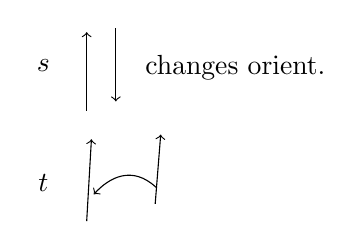
\begin{tikzpicture}
\node at (-.55,0.57) {$s$};
\draw[->] (0,0) -- (0,1);
\draw[->] (.37,1.05) -- (.37,.12);
\node[anchor=west] at (.62,.55) {changes orient.};
\node at (-.55,-.92) {$t$};
\draw[->] (0,-1.40) -- (.06,-.36);
\draw[->] (.87,-1.18) -- (.94,-.30);
\draw[->] (.88,-.97) .. controls (.58,-.69) and (.29,-.84) .. (.09,-1.06);
\end{tikzpicture}}\endgroup}
\end{GelfandAdjacentEvidence}
\begin{GelfandAdjacentEvidence}{GELFAND-P000510}{3}

\[
\left(\int_0^{i\infty}+\int_{s(0)}^{s(i\infty)}\right)\Phi(z)\,dz
=0=\left(\int_0^{i\infty}+\int_{t(0)}^{\ldots}+\ldots\right)
\]
\[
\underline{\tau_k(\Phi)+(-1)^k\tau_{w-k}(\varphi)=0}
\qquad\text{(also follows from the funct. eq.)}
\]
\[
\int_0^{i\infty}\varphi(z)
\left[z^k+z^{w-k}(z-1)^k+(-1)^k(z-1)^{w-k}\right]\,dz=0.
\]
This gives the sought lin. eq. for $\tau_k$.
\[
S_{w+2}=\text{$R$-space of forms $\varphi$ with real coeffs.}
\]
\[
S_{w+2}\longrightarrow R
\]
\SourceFigure{GELFAND-P000510}{period-parity-map}{%
\begingroup\color{black}\GelfandFitDiagram{\begin{tikzpicture}
\node (form) at (0,0) {$\varphi$};
\node[anchor=west] (even) at (.76,.52) {$\dfrac1i(\tau_0(\Phi),\tau_2(\varphi),\ldots)$};
\node[anchor=west] (odd) at (.76,-.59) {$(\tau_1(\varphi),\ldots,\tau_{w-1}(\varphi))$};
\draw[->] (form.east) -- (even.west);
\draw[->] (form.east) -- (odd.west);
\end{tikzpicture}}\endgroup}
\end{GelfandAdjacentEvidence}
\begin{GelfandAdjacentEvidence}{GELFAND-P000510}{4}


In the period spaces take the subspaces given by the eqs.
\SourceFigure{GELFAND-P000510}{solution-space-map}{%
\(\displaystyle
S_{w+2}
\left.\begin{array}{cc}\nearrow&S^+\\\searrow&S^-\end{array}\right\}
\underset{\mathrm{def}}{=}
\)\par\smallskip
spaces of solutions of the eqs. of Sh.-Eich.}
\end{GelfandAdjacentEvidence}
\begin{GelfandAdjacentEvidence}{GELFAND-P000510}{5}


\uuline{Theorem}.
\[
\begin{aligned}
\text{a)}\quad&S_{w+2}\overset{\sim}{\longrightarrow}S^-\\
\text{b)}\quad&S_{w+2}\hookrightarrow S^+\qquad
\text{embedding}\quad\operatorname{codim}1.
\end{aligned}
\]

\uuline{Theorem}.
\SourceFigure{GELFAND-P000510}{hecke-period-map}{%
\begingroup\color{black}\GelfandFitDiagram{\begin{tikzpicture}
\node (source) at (0,0) {$S_{w+2}$};
\node (target) at (1.95,0) {$S^-$};
\draw[->] (source.east) -- node[above] {$\sim$} (target.west);
\node at (0,-.66) {$T_p$};
\node[draw,ellipse,inner sep=2pt] at (1.95,-.66) {$T_p^-$};
\node[anchor=west] at (2.65,-.66) {(Hecke op.).};
\node[anchor=north] at (1.95,-.98) {matrix over $\mathbb Z[\lambda_p]$};
\end{tikzpicture}}\endgroup}
\end{GelfandAdjacentEvidence}
\begin{GelfandAdjacentEvidence}{GELFAND-P000510}{6}


Here
\[
(\Phi\mid T_p)(z)=p^{w+1}\varphi(pz)
-p^{-1}\sum_{k=0}^{p-1}\varphi\left(\frac{z+k}{p}\right)
\]
\SourceFigure{GELFAND-P000510}{hecke-minus}{A minus sign is written before $p^{-1}\sum$.}
\end{GelfandAdjacentEvidence}
\begin{GelfandAdjacentEvidence}{GELFAND-P000510}{7}

Eigenfns. of the Hecke op. $\Leftrightarrow$
[Crossed out: \Incomplete{GELFAND-P000510}{hecke-cancellation}{The reading under the heavy strikeout is unresolved.}
\end{GelfandAdjacentEvidence}
]
factor into an Euler prod.

$T_p^-$ — expression in terms of periods (the lin. form is uniquely det.)

\uline{Application}.
\[
\begin{aligned}
w&=10,\qquad S_{12}=R\cdot e^{2\pi iz}
 \prod_{n=1}^\infty(1-e^{2\pi inz})^{24}\\
 &=R\left(\sum_{n=1}^\infty\tau(n)e^{2\pi inz}\right)
\end{aligned}
\]
\hfill (Ramanujan fn.)\par

\uwave{Ramanujan identity}
\[
\tau(n)\equiv\sum_{d\mid n}d^{11}\pmod{691}
\]


\Needspace{7\baselineskip}
\begin{GelfandAdjacentEvidence}{GELFAND-P000511}{1}
\SourcePage{GELFAND-P000511}{unlabelled}
\uuline{Measures}.
\[
\begin{aligned}
P^+(x)&=\frac{i}{\omega^+}\operatorname{Im}\int_x^{i\infty}\varphi(z)\,dz,\\
P^-(x)&=\frac{1}{\omega^-}\operatorname{Re}\int_x^{i\infty}\Phi(z)\,dz
\end{aligned}
\]
\[
\mu_\varphi^\pm\bigl(a+(p^{m+1})\bigr)
\underset{\mathrm{def}}{=}
\varrho^{-m}P^\pm\left(\frac{a}{p^{m+1}}\right)
-p^w\varrho^{-(m+1)}P^\pm\left(\frac{a}{p^m}\right)
\]
\Unclear{GELFAND-P000511}{measure-overwriting}{The $P$ and the exponent on $p$ in the last term are overwritten. Provisionally read as $P^\pm(a/p^m)$.}
\end{GelfandAdjacentEvidence}
\begin{GelfandAdjacentEvidence}{GELFAND-P000511}{2}

measures with alg. values, and one can complete.
\Unclear{GELFAND-P000511}{measure-note}{The last Russian verb is provisionally read “пополнять”. Another possible reading is “пополнить”.}
\end{GelfandAdjacentEvidence}
\begin{GelfandAdjacentEvidence}{GELFAND-P000511}{3}


\uwave{Growth}. $P^\pm$ have bounded denominators.
They may arise from $\varrho$.
\[
\varrho^2-\lambda_p\varrho+p^{w+1}=0
\]
\[
\begin{cases}
\varrho_1\cdot\varrho_2=p^{w+1}\\
\varrho_1+\varrho_2=\lambda_p.
\end{cases}
\]
Typ. case: \uwave{\mbox{$\lambda_p$} copr. to \mbox{$p$}}
$\Rightarrow$ one root gives a bounded measure, the other a growing one!

Unknown relation [crossed out:
\Incomplete{GELFAND-P000511}{cancelled-middle}{The reading between “relation” and the next symbol is unresolved.}
\end{GelfandAdjacentEvidence}
\begin{GelfandAdjacentEvidence}{GELFAND-P000511}{4}
]
$\lambda_p$ and $p$.

\uline{Integrals} (Mellin transf. of $p$-adic char.)
\[
\ldots\int_{\mathbb Z_p^*}\chi\,d\mu_\Phi^\pm
\]
Manin can do it only for a char. of finite ord. $\chi:\mathbb Z_p^*\to K^*$,
$\chi^m=1$ and primitive.

\uline{Theorem}
\[
\ldots\int_{\mathbb Z_p^*}\chi\,d\mu_\varphi^\pm=\ldots L_\varphi(1,\chi),
\]
where
\[
L_\Phi(s,\chi)=\sum_{n=1}^\infty\chi(n)a_n n^{-s}
\]
\[
\ldots\dot L_\varphi(1,\chi)
=\ldots\int_{R_+^*}\varphi_\chi(z)\,dz,
\qquad\text{where }\Phi_\chi=\sum\chi(n)a_ne^{2\pi inz}.
\]
\Unclear{GELFAND-P000511}{l-dot}{A separate dot is visible above $L$ in the manuscript. Its meaning is unresolved.}
\end{GelfandAdjacentEvidence}
\begin{GelfandAdjacentEvidence}{GELFAND-P000511}{5}


\uline{On Lichtenbaum’s conjectures}: \uwave{on the connection of \mbox{$K$}-groups of alg. fields with
\mbox{$\zeta$}-fns. at int. points.}
\[
\sum_{n=1}^\infty\frac{1}{n^2}=\frac{\pi^2}{6},\qquad
\underset{\text{For the first time there is a conjecture}}{%
\sum_{n=1}^\infty\frac{1}{n^3}=2\pi^2\lvert K_4\mathbb Z\rvert\cdot e_5(\alpha_5)}
\]
$\alpha_5$ — a generator of $K_5\mathbb Z$. (of the free part)

$e_5$ — a homom. into the real numbers (a certain one)

It is unproved that $\displaystyle\sum_1^\infty\frac{1}{n^3}$ is transcend.
Euler’s const. also unproved.

\Incomplete{GELFAND-P000511}{cancelled-bottom}{The text inside the rectangle is heavily crossed out. Its reading is unresolved.}
\end{GelfandAdjacentEvidence}



\Needspace{7\baselineskip}
\begin{GelfandAdjacentEvidence}{GELFAND-P000512}{1}
\SourcePage{GELFAND-P000512}{unlabelled}
\Unclear{GELFAND-P000512}{upper-right-edge}{Clipped strokes are visible at the upper right. The reading is unresolved.}
\end{GelfandAdjacentEvidence}
\begin{GelfandAdjacentEvidence}{GELFAND-P000512}{2}


\uuline{24.9.73.}\qquad\uuline{Gelfand Sem.}

\uwave{Pincus}\quad
\uline{Douglas, Coburn, Vilneyer and Singer}\quad
\uwave{Helton and Roger Howe. (Howe)}
\Unclear{GELFAND-P000512}{upper-names}{The surname after Coburn is provisionally transcribed “Вилнейер” and romanized “Vilneyer”. The middle letters run together.}
\end{GelfandAdjacentEvidence}
\begin{GelfandAdjacentEvidence}{GELFAND-P000512}{3}


(interesting work in funct. analysis).

\uline{Theorem} (\uwave{Helton, How}). close to the work of Krein, Gohberg, Simonenko, etc.

Let $B$ — a bilin. form on 2 polynomials
[inserted above the line: of 2 var.], with
\[
B(P_1(Q),P_2(Q))=0,
\]
if $P_1(z),P_2(z)$ — polyn. in one var. $z$,
and $Q$ — a polyn. in any number of var. Then
\[
B(R,S)=L(\{R,S\}),\qquad \{R,S\}\ \text{— Poisson bracket}
\]
\uwave{\mbox{$L$} — lin. form.}
\SourceFigure{GELFAND-P000512}{two-variable-insertion}{The insertion “of 2 var.” is circled and points to the place after “polynomials”.}
\end{GelfandAdjacentEvidence}
\begin{GelfandAdjacentEvidence}{GELFAND-P000512}{4}


\begin{center}— · —\end{center}
Let $U,V$ — self-adj. and commuting mod nuclear operators.
Then
\[
\operatorname{Tr}\{[R(U,V),S(U,V)]\}=\iint\{R,S\}\,d\sigma
\]
$R,S$ — polynomials. The order of $U$ and $V$ in them is immaterial.

\begin{center}— · —\end{center}
\uline{Book}\quad\uuline{by Douglas}\quad\uwave{Banach algebras technique.}

$\Rightarrow$ in the $p$-adic case suitably chosen normed rings are needed in place of diff. operators.

\begin{center}— · —\end{center}
\uline{Kirillov.}

\uline{L. Brown, R. Douglas, P. Fillmore.}

\uline{Extensions of Banach algebras (of a nontraditional type).}

$\mathcal K$ — alg. of comp. operators on a sep. Hilbert space.

\uline{Def. 1.}
\[
0\to\mathcal K\to\mathcal A\to C(X)\to0,\qquad X\ \text{— compact}
\]
Exts. form a group $\operatorname{Ext}(X)=\operatorname{Ext}_1(X)$.

\uline{Another definition gives the same group:}

\uline{Def. 2.}
\SourceFigure{GELFAND-P000512}{embedding-bracket}{%
\begingroup\color{black}\GelfandFitDiagram{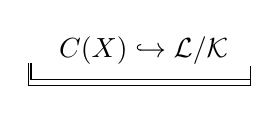
\begin{tikzpicture}
\node[inner xsep=8pt] (embedding) {$C(X)\hookrightarrow\mathcal L/\mathcal K$};
\draw ([xshift=-2pt,yshift=4pt]embedding.south west) |-
 ([yshift=-2pt]embedding.south east) -- ++(0,5pt);
\draw ([xshift=-3pt,yshift=4pt]embedding.south west) |-
 ([yshift=-4pt]embedding.south east) -- ++(0,7pt);
\end{tikzpicture}}\endgroup}
\end{GelfandAdjacentEvidence}
\begin{GelfandAdjacentEvidence}{GELFAND-P000512}{5}


1) consider all embeddings.

2) identify embeddings differing by a unit. op. (unit. eq. $UAU^{-1}$).

3) Embeddings of the form $C(X)\to\mathcal L\to\mathcal L/\mathcal K$ are regarded as triv.

Equiv. classes then form a group.
\SourceFigure{GELFAND-P000512}{parallel-embeddings}{%
\begingroup\color{black}\GelfandFitDiagram{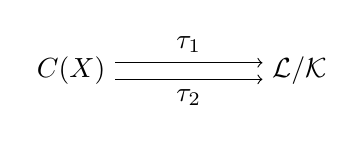
\begin{tikzpicture}
\node (functions) at (0,0) {$C(X)$};
\node (quotient) at (2.9,0) {$\mathcal L/\mathcal K$};
\draw[->] ([yshift=3pt]functions.east) -- node[above] {$\tau_1$} ([yshift=3pt]quotient.west);
\draw[->] ([yshift=-3pt]functions.east) -- node[below] {$\tau_2$} ([yshift=-3pt]quotient.west);
\end{tikzpicture}}\endgroup}
\end{GelfandAdjacentEvidence}
\begin{GelfandAdjacentEvidence}{GELFAND-P000512}{6}

$\tau_1\oplus\tau_2$ already in $H_1\oplus H_2\cong H$

Functor
\SourceFigure{GELFAND-P000512}{functor-arrow}{%
\begingroup\color{black}\GelfandFitDiagram{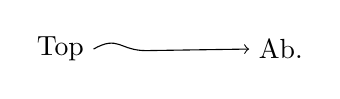
\begin{tikzpicture}
\node (top) at (0,0) {\uwave{Top}};
\node (ab) at (2.8,0) {\uwave{Ab.}};
\draw[->] (top.east) .. controls (.74,.18) and (.75,-.02) .. (1.09,-.02) -- (ab.west);
\end{tikzpicture}}\endgroup}
\end{GelfandAdjacentEvidence}
\begin{GelfandAdjacentEvidence}{GELFAND-P000512}{7}


\uline{Main result:} the functor $\operatorname{Ell}(X)$ reduces to
$\operatorname{Ext}(X)$ (answer to a question of Atiyah).
\[
\operatorname{Ext}_{1-n}(X)=
\operatorname{Ext}\left(
\underset{\substack{\vert\\\text{\mbox{$n$}-fold suspension}}}{S^nX}
\right)
\]
\SourceFigure{GELFAND-P000512}{suspension-pointer}{A short stroke under $S^nX$ points to the label.}
\end{GelfandAdjacentEvidence}



\Needspace{7\baselineskip}
\begin{GelfandAdjacentEvidence}{GELFAND-P000513}{1}
\SourcePage{GELFAND-P000513}{14}
\uuline{Th. 1.} Exact seq.
\[
\operatorname{Ext}_1(A)\to\operatorname{Ext}_1(X)\to
\operatorname{Ext}_1(X/A)\to\operatorname{Ext}_0(A)\to\ldots
\]
$A\subset X$

\uuline{Th. 2.} There is a pairing
\[
K^1\times\operatorname{Ext}_1\to\operatorname{Ext}_0
\]
\[
K^1(X\times Y)\times\operatorname{Ext}_1(X)\to K^0(Y)
\]
\sout{The functor \mbox{$\operatorname{Ext}_1$} is computed for all}
\Incomplete{GELFAND-P000513}{cancelled-upper-end}{The end of the crossed-out line is illegible.}
\end{GelfandAdjacentEvidence}
\begin{GelfandAdjacentEvidence}{GELFAND-P000513}{2}

\Unclear{GELFAND-P000513}{cancelled-upper-word}{The crossed-out verb is provisionally read as “computed”.}
\end{GelfandAdjacentEvidence}
\begin{GelfandAdjacentEvidence}{GELFAND-P000513}{3}


\SourceFigure{GELFAND-P000513}{ext-underbracket}{%
\begingroup\color{black}\GelfandFitDiagram{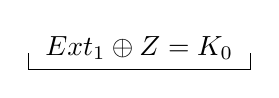
\begin{tikzpicture}
\node[inner xsep=6pt] (identity) {$\operatorname{Ext}_1\oplus Z=K_0$};
\draw ([yshift=6pt]identity.south west) |- (identity.south east) -- ++(0,6pt);
\end{tikzpicture}}\endgroup}
\end{GelfandAdjacentEvidence}
\begin{GelfandAdjacentEvidence}{GELFAND-P000513}{4}

for simpl. complexes.
\Unclear{GELFAND-P000513}{ext-operation}{The sign before $Z$ is heavily retraced. Provisionally set as $\oplus$. It could be $\otimes$.}
\end{GelfandAdjacentEvidence}
\begin{GelfandAdjacentEvidence}{GELFAND-P000513}{5}


\uline{Example of an extension}.
\[
0\to\mathcal K\to C^*(\text{„}ax+b\text{”})\to C(\infty)\to0
\]
\[
\operatorname{Ext}(\infty)=Z+Z.
\]
What is this pair of numbers for a specific op.?

\begin{center}— · —\end{center}
\sout{\mbox{$X=S^1$}}
\SourceFigure{GELFAND-P000513}{cancelled-torus}{$X=S^1$ is crossed out on the left.}
\end{GelfandAdjacentEvidence}
\begin{GelfandAdjacentEvidence}{GELFAND-P000513}{6}

\[
X=\mathbb T=S^1
\]
\SourceFigure{GELFAND-P000513}{torus-generator}{%
\begingroup\color{black}\GelfandFitDiagram{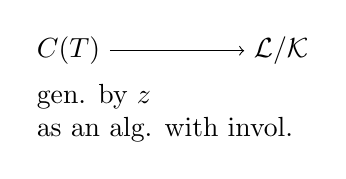
\begin{tikzpicture}
\node (circle) at (0,0) {$C(\mathbb T)$};
\node (quotient) at (2.7,0) {$\mathcal L/\mathcal K$};
\draw[->] (circle.east) -- (quotient.west);
\node[anchor=north west,align=left] at (circle.south west)
  {gen. by $z$\\as an alg. with invol.};
\end{tikzpicture}}\endgroup}
\end{GelfandAdjacentEvidence}
\begin{GelfandAdjacentEvidence}{GELFAND-P000513}{7}


Let $T$ — the image of $z$.
\[
TT^*=1\bmod\mathcal K
\]
\uwave{up to unit. equiv. and \mbox{$\bmod\ 1+\mathcal K$}.}

\uline{Answer:}\quad\uuline{index}\quad(classific.).

\begin{center}— · —\end{center}
\uline{Th.}
\[
\left\{\underset{\substack{\vert\\\text{norm.}}}{N}+\mathcal K\right\}
\]
is norm-closed among all op.,
\SourceFigure{GELFAND-P000513}{normal-pointer}{A short stroke connects $N$ to the label “norm.” below.}
\end{GelfandAdjacentEvidence}
\begin{GelfandAdjacentEvidence}{GELFAND-P000513}{8}


but \sout{\mbox{$N_1N_2=N_2N_1$}}
pairs $\{N_1+K_1,\ N_2+K_2\}$ with cond. $N_1N_2=N_2N_1$
[inserted and circled at the left: not closed] in the set of all pairs of this kind.
\SourceFigure{GELFAND-P000513}{pair-revisions}{The equality is crossed out before “pairs”. The insertion at the left is circled.}
\end{GelfandAdjacentEvidence}
\begin{GelfandAdjacentEvidence}{GELFAND-P000513}{9}

\Unclear{GELFAND-P000513}{cancelled-notclosed}{The crossed-out word below the circle is provisionally read as “not closed”.}
\end{GelfandAdjacentEvidence}


\uuline{Next time:}\quad\uwave{Fuchs’s talk}\quad\uwave{pres. on Mishchenko}.

\uuline{Fuchs.}\qquad\uline{Quillen}\qquad\uwave{Higher algebraic K-theory I}

(Proc. of symp. on $K$-theory)

\uline{Introduction.} $M$ — a category (abelian or spec. additive).
We define $K_i(M)$.

\uline{Constructions}

$QM$ — cat. of quotients $\Rightarrow$ classif. space $BQM$ $\Rightarrow$
\[
\Rightarrow\quad K_i(M)=\pi_{i+1}(BQM).
\]

\uline{Essential part.}

A simpl. object in a category $S$ — a contravar. functor $\mathrm{Ord}\to S$,
where $\mathrm{Ord}$ — the can. category of nonnegative integers.


\Needspace{7\baselineskip}
\begin{GelfandAdjacentEvidence}{GELFAND-P000514}{1}
\SourcePage{GELFAND-P000514}{unlabelled}
\[
\mathrm{Ord}^{\circ}\longrightarrow S
\]
\Unclear{GELFAND-P000514}{top-functor}{There is a small oval above $\mathrm{Ord}$. Provisionally set as $\circ$. It could also be $o$ or $0$.}
\end{GelfandAdjacentEvidence}
\begin{GelfandAdjacentEvidence}{GELFAND-P000514}{2}


(Functor always means covar. functor).

$\mathrm{Ord}$\quad objects — $0,1,2,3,\ldots$

Morphism [crossed out:
\Incomplete{GELFAND-P000514}{upper-cancellation}{The reading under the strikeout is unresolved.}
\end{GelfandAdjacentEvidence}
\begin{GelfandAdjacentEvidence}{GELFAND-P000514}{3}
]
$p\to q$ is called a monotonically nondecr. map
\[
(0,1,\ldots,p)\longrightarrow(0,1,\ldots,q)
\]
All are repr. as compositions of morphisms of 2 kinds:

\SourceFigure{GELFAND-P000514}{order-maps}{%
\begingroup\color{black}\GelfandFitDiagram{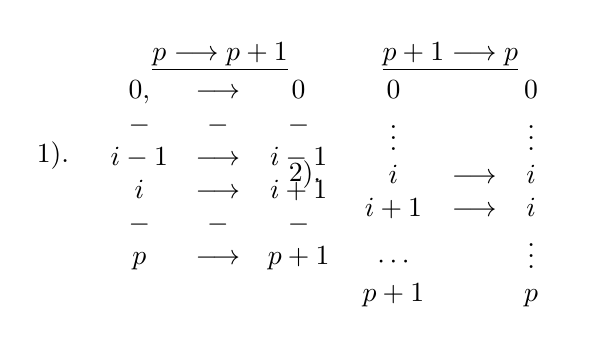
\begin{tikzpicture}
\node[anchor=north west] at (0,0) {$1).\quad
\begin{array}{c}
\underline{p\longrightarrow p+1}\\[2pt]
\begin{array}{@{}ccc@{}}
0,&\longrightarrow&0\\
-&-&-\\
i-1&\longrightarrow&i-1\\
i&\longrightarrow&i+1\\
-&-&-\\
p&\longrightarrow&p+1
\end{array}
\end{array}$};
\node[anchor=north west] at (3.2,0) {$2).\quad
\begin{array}{c}
\underline{p+1\longrightarrow p}\\[2pt]
\begin{array}{@{}ccc@{}}
0&&0\\
\vdots&&\vdots\\
i&\longrightarrow&i\\
i+1&\longrightarrow&i\\
\cdots&&\vdots\\
p+1&&p
\end{array}
\end{array}$};
\end{tikzpicture}}\endgroup}
\end{GelfandAdjacentEvidence}
\begin{GelfandAdjacentEvidence}{GELFAND-P000514}{4}


To specify a simpl. obj. it suffices to give a seq. of objects
\[
S_0,S_1,S_2,\ldots
\]
and morphisms
\SourceFigure{GELFAND-P000514}{face-ladder}{%
\begingroup\color{black}\GelfandFitDiagram{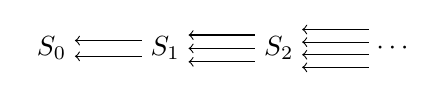
\begin{tikzpicture}[x=.78cm]
\node at (0,0) {$S_0$};
\node at (1.85,0) {$S_1$};
\node at (3.70,0) {$S_2$};
\node at (5.55,0) {$\cdots$};
\foreach \y in {-.10,.10} {\draw[<-] (.38,\y) -- (1.47,\y);}
\foreach \y in {-.17,0,.17} {\draw[<-] (2.23,\y) -- (3.32,\y);}
\foreach \y in {-.24,-.08,.08,.24} {\draw[<-] (4.08,\y) -- (5.16,\y);}
\end{tikzpicture}}\endgroup}
\end{GelfandAdjacentEvidence}
\begin{GelfandAdjacentEvidence}{GELFAND-P000514}{5}

(correspond to embeddings of type 1))

and
\SourceFigure{GELFAND-P000514}{degeneracy-ladder}{%
\begingroup\color{black}\GelfandFitDiagram{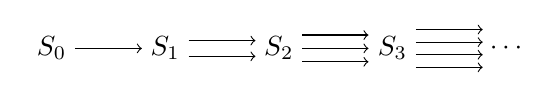
\begin{tikzpicture}[x=.78cm]
\node at (0,0) {$S_0$};
\node at (1.85,0) {$S_1$};
\node at (3.70,0) {$S_2$};
\node at (5.55,0) {$S_3$};
\node at (7.40,0) {$\cdots$};
\draw[->] (.38,0) -- (1.47,0);
\foreach \y in {-.10,.10} {\draw[->] (2.23,\y) -- (3.32,\y);}
\foreach \y in {-.17,0,.17} {\draw[->] (4.08,\y) -- (5.16,\y);}
\foreach \y in {-.24,-.08,.08,.24} {\draw[->] (5.93,\y) -- (7.02,\y);}
\end{tikzpicture}}\endgroup}
\end{GelfandAdjacentEvidence}
\begin{GelfandAdjacentEvidence}{GELFAND-P000514}{6}

(corr. to maps of type 2))

(The relations must be satisfied).

\hspace*{3em}they are easy to write down

$S$ — either the cat. of sets or the cat. of top. spaces.

Groups, smooth manifolds, etc. are also possible.

\uuline{Important example:} sing. complex of a top. space. $S$ — cat. of sets.

$X$ — top. space. Denote by $S_q$ — all sing. simplices of $X$
\SourceFigure{GELFAND-P000514}{lower-notation}{The Russian abbreviation reads “Обозн.”.}
\end{GelfandAdjacentEvidence}
\begin{GelfandAdjacentEvidence}{GELFAND-P000514}{7}


(cont. maps $\Delta^q\to X$, where
\[
\Delta^q=\{(x_1,\ldots,x_{q+1})\in R^{q+1},\quad x_i\geq0,\quad\sum x_i=1\}.
\]
\SourceFigure{GELFAND-P000514}{singular-parenthesis}{An opening parenthesis precedes “cont. maps”. There is no visible matching parenthesis before the next formula.}
\end{GelfandAdjacentEvidence}
\begin{GelfandAdjacentEvidence}{GELFAND-P000514}{8}


\[
\exists\ \delta_i:\Delta^{q-1}\longrightarrow\Delta^q
\]
canon. map onto the $i$-th face (vertices ordered)
\Unclear{GELFAND-P000514}{lower-face-symbol}{The letter with index $i$ is provisionally set as $\delta_i$. It could be $\gamma_i$.}
\end{GelfandAdjacentEvidence}
\begin{GelfandAdjacentEvidence}{GELFAND-P000514}{9}


Sing. simplex — composition
\[
\Delta^{q-1}\longrightarrow\Delta^q\longrightarrow X
\]
\Unclear{GELFAND-P000514}{lower-singular-abbreviation}{The initial Russian abbreviation is provisionally read as “Син.”. Its last letter is uncertain.}
\end{GelfandAdjacentEvidence}
\begin{GelfandAdjacentEvidence}{GELFAND-P000514}{10}


We get $q+1$ maps
\SourceFigure{GELFAND-P000514}{face-family}{%
\begingroup\color{black}\GelfandFitDiagram{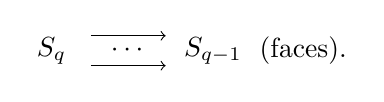
\begin{tikzpicture}
\node at (0,0) {$S_q$};
\node at (2.05,0) {$S_{q-1}$};
\draw[->] (.50,.19) -- (1.45,.19);
\node at (.96,0) {$\cdots$};
\draw[->] (.50,-.19) -- (1.45,-.19);
\node[anchor=west] at (2.52,0) {(faces).};
\end{tikzpicture}}\endgroup}
\end{GelfandAdjacentEvidence}
\begin{GelfandAdjacentEvidence}{GELFAND-P000514}{11}


\SourceFigure{GELFAND-P000514}{degeneracy-family}{%
\begingroup\color{black}\GelfandFitDiagram{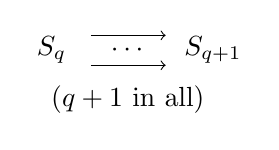
\begin{tikzpicture}
\node at (0,0) {$S_q$};
\node at (2.05,0) {$S_{q+1}$};
\draw[->] (.50,.19) -- (1.45,.19);
\node at (.96,0) {$\cdots$};
\draw[->] (.50,-.19) -- (1.45,-.19);
\node[anchor=north] at (.97,-.32) {($q+1$ in all)};
\end{tikzpicture}}\endgroup}
\end{GelfandAdjacentEvidence}

from $\Delta^{q+1}\longrightarrow\Delta^q$\quad affine projections
($i$-th identifies the $i$-th vertex with the $(i+1)$-st).

\begin{center}— · —\end{center}


\Needspace{7\baselineskip}
\begin{GelfandAdjacentEvidence}{GELFAND-P000515}{1}
\SourcePage{GELFAND-P000515}{15}
\uline{Realization}.

Let $S$ — the cat. of sets or top. spaces.

A top. space is associated with a simpl. obj. in the cat. of sets or top. spaces.

\uwave{Elements of} [inserted above the line, circled: the set] \uwave{\mbox{$S_i$} are called simplices}
\SourceFigure{GELFAND-P000515}{set-insertion}{The circled abbreviation for “set” points to the place after “Elements”.}
\end{GelfandAdjacentEvidence}
\begin{GelfandAdjacentEvidence}{GELFAND-P000515}{2}


\uwave{The images of arrows from left to right are called degenerate simplices.}

\uwave{The others are called nondegenerate.} \uwave{Arrows from right to left take nondeg. to nondegenerate simplices.}
\SourceFigure{GELFAND-P000515}{nondegenerate-faces}{The manuscript states that the right-to-left arrows take nondeg. to nondegenerate simplices.}
\end{GelfandAdjacentEvidence}
\begin{GelfandAdjacentEvidence}{GELFAND-P000515}{3}


Consider $\Delta^q\times S_q^0$

\hspace*{3em}nondeg. simpl. from $S_q$.\qquad ($S_q^0$ — a discrete top. space).

In $\coprod_q\Delta^q\times S_q^0$ (disjoint union) an identification.
\[
\Delta^{q-1}\times s,\qquad s\in S_{q-1}^0
\]
is identified with part of $\Delta^q\times s'$, $s'\in S_q^0$,
when $s$ — the image of $s'$ under the map ($i$-th)
\[
S_{q-1}\overset{i}{\longleftarrow}S_q\qquad
\text{($i$-th face)}
\]
\SourceFigure{GELFAND-P000515}{gluing-membership}{A prime is visible in the membership condition: $s'\in S_q^0$.}
\end{GelfandAdjacentEvidence}
\begin{GelfandAdjacentEvidence}{GELFAND-P000515}{4}


\uline{We get a top. space.} \uline{This is a cell space} (the interiors are left unglued).

But: boundary points can be glued together (so it is not a simplicial space).

The same ex. if $S$ — top. spaces. A top. struct. no longer arises,
since in $\Delta^q\times S_q^0$ there is the direct product top.
\SourceFigure{GELFAND-P000515}{topological-wording}{The manuscript reads “A top. struct. no longer arises”.}
\end{GelfandAdjacentEvidence}
\begin{GelfandAdjacentEvidence}{GELFAND-P000515}{5}


\uuline{Ex.:} for a good top. space the realization of the sing.
[crossed out: \Incomplete{GELFAND-P000515}{middle-cancellation}{The reading under the strikeout is unresolved.}
\end{GelfandAdjacentEvidence}
\begin{GelfandAdjacentEvidence}{GELFAND-P000515}{6}
]
complex is homotopy equiv. to $X$.

To reconstr. a polyhedron, take for $S_i$ the aff. maps of simplices into it
\SourceFigure{GELFAND-P000515}{polyhedron-abbreviation}{The Russian abbreviation before “polyhedron” reads “восстан.”.}
\end{GelfandAdjacentEvidence}
\begin{GelfandAdjacentEvidence}{GELFAND-P000515}{7}

\SourceFigure{GELFAND-P000515}{polyhedron-sketch}{%
\begingroup\color{black}\GelfandFitDiagram{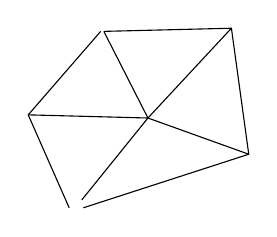
\begin{tikzpicture}[x=.02cm,y=-.02cm]
\draw (64,25)--(145,23)--(156,103)--(51,137);
\draw (42,137)--(16,78)--(62,25);
\draw (92,80)--(64,25);
\draw (92,80)--(145,23);
\draw (92,80)--(156,103);
\draw (92,80)--(50,132);
\draw (92,80)--(16,78);
\end{tikzpicture}}\endgroup}
\end{GelfandAdjacentEvidence}
\begin{GelfandAdjacentEvidence}{GELFAND-P000515}{8}


\uwave{Realization commutes with multiplication.}
\SourceFigure{GELFAND-P000515}{product-diagrams}{%
\begingroup\color{black}\GelfandFitDiagram{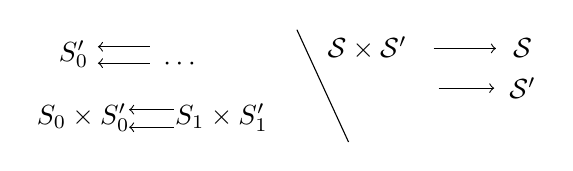
\begin{tikzpicture}[x=.72cm,y=.72cm]
\node at (.25,0) {$S'_0$};
\node at (2.12,-.18) {$\cdots$};
\draw[<-] (.68,.13) -- (1.60,.13);
\draw[<-] (.68,-.16) -- (1.60,-.16);
\node at (.42,-1.12) {$S_0\times S'_0$};
\node at (2.86,-1.12) {$S_1\times S'_1$};
\draw[<-] (1.23,-.98) -- (2.02,-.98);
\draw[<-] (1.23,-1.29) -- (2.02,-1.29);
\draw (4.19,.43) -- (5.10,-1.55);
\node at (5.43,.10) {$\mathcal S\times\mathcal S'$};
\node at (8.17,.10) {$\mathcal S$};
\node at (8.17,-.60) {$\mathcal S'$};
\draw[->] (6.60,.10) -- (7.70,.10);
\draw[->] (6.69,-.60) -- (7.67,-.60);
\end{tikzpicture}}\endgroup}
\end{GelfandAdjacentEvidence}
\begin{GelfandAdjacentEvidence}{GELFAND-P000515}{9}


hence
\SourceFigure{GELFAND-P000515}{realization-projections}{%
\begingroup\color{black}\GelfandFitDiagram{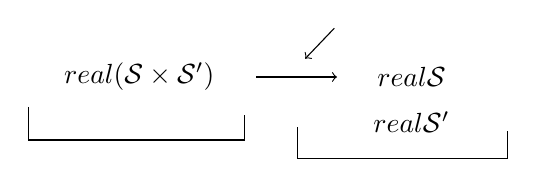
\begin{tikzpicture}[x=.86cm,y=.86cm]
\node at (1.65,0) {$\operatorname{real}(\mathcal S\times\mathcal S')$};
\node at (5.67,0) {$\operatorname{real}\mathcal S$};
\node at (5.67,-.66) {$\operatorname{real}\mathcal S'$};
\draw[->] (3.38,0) -- (4.57,0);
\draw[->] (4.53,.72) -- (4.10,.27);
\draw (.01,-.44) -- (.01,-.93) -- (3.20,-.93) -- (3.20,-.56);
\draw (3.98,-.74) -- (3.98,-1.20) -- (7.09,-1.20) -- (7.09,-.80);
\end{tikzpicture}}\endgroup}
\end{GelfandAdjacentEvidence}
\begin{GelfandAdjacentEvidence}{GELFAND-P000515}{10}


and together they form
\SourceFigure{GELFAND-P000515}{realization-product-map}{%
\begingroup\color{black}\GelfandFitDiagram{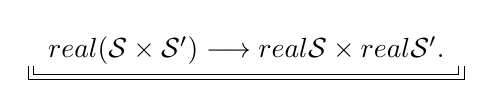
\begin{tikzpicture}
\node[inner xsep=5pt] (product) {$\operatorname{real}(\mathcal S\times\mathcal S')
 \longrightarrow\operatorname{real}\mathcal S\times\operatorname{real}\mathcal S'.$};
\draw ([yshift=3pt]product.south west) |- (product.south east) -- ++(0,3pt);
\draw ([xshift=-2pt,yshift=3pt]product.south west) |-
 ([xshift=2pt,yshift=-2pt]product.south east) -- ++(0,5pt);
\end{tikzpicture}}\endgroup}
\end{GelfandAdjacentEvidence}
\begin{GelfandAdjacentEvidence}{GELFAND-P000515}{11}


\uuline{Prop.} \uwave{It turns out to be} — \uuline{a homeomorphism.}

\uline{Example.}
\SourceFigure{GELFAND-P000515}{ordered-segment}{%
\begingroup\color{black}\GelfandFitDiagram{\begin{tikzpicture}
\draw (0,0)--(1.2,0);
\draw (0,-.10)--(0,.10);
\draw (1.2,-.10)--(1.2,.10);
\end{tikzpicture}}\endgroup\quad Ordered segment.}
\end{GelfandAdjacentEvidence}
\begin{GelfandAdjacentEvidence}{GELFAND-P000515}{12}


$S^0$ — 2 elements

$S^1$ — 3 elem. (counting degenerate ones)

$S^p=(p+2)$ elem. $i$-th:
\[
[0,i-1]\longrightarrow0,\qquad[i,p]\longrightarrow1
\]
\Unclear{GELFAND-P000515}{lower-overwritten-exponent}{The raised sign to the right of $S$ is heavily retraced. Provisionally set as $p$. A short stroke appears above $S$ on the left.}
\end{GelfandAdjacentEvidence}
\begin{GelfandAdjacentEvidence}{GELFAND-P000515}{13}


$S_p\times S_p$
\Unclear{GELFAND-P000515}{product-foot-marks}{Faint detached strokes follow the product. Their reading is unresolved.}
\end{GelfandAdjacentEvidence}


(next time.)


\Needspace{7\baselineskip}
\begin{GelfandAdjacentEvidence}{GELFAND-P000516}{1}
\SourcePage{GELFAND-P000516}{unlabelled}
\S2. \uline{Classif. space in a category.}

$C$ — a category (small). Associated to it is its nerve $NC$ (simpl. object of the cat. of sets).
\[
NC_q=\{\text{[?]}\quad X_0\longrightarrow\cdots\longrightarrow X_q\}
\qquad\text{set of such diagrams}
\]
\Unclear{GELFAND-P000516}{nerve-blot}{An overwritten mark is visible after the opening brace before $X_0$. The reading is unresolved.}
\end{GelfandAdjacentEvidence}
\begin{GelfandAdjacentEvidence}{GELFAND-P000516}{2}


\[
\underline{NC_q\longrightarrow NC_{q-1}}
\]

\uline{0th}
\SourceFigure{GELFAND-P000516}{discard-face}{%
\begingroup\color{black}\GelfandFitDiagram{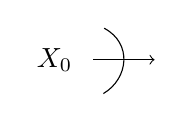
\begin{tikzpicture}[baseline=(object.base)]
\node (object) at (0,0) {$X_0$};
\draw[->] (.49,0) -- (1.27,0);
\draw (.63,.40) .. controls (.99,.21) and (.94,-.24) .. (.62,-.43);
\end{tikzpicture}}\endgroup\qquad (discard it).}
\end{GelfandAdjacentEvidence}
\begin{GelfandAdjacentEvidence}{GELFAND-P000516}{3}


\uline{\mbox{$q$}th} — discard $X_q$

\uuline{\mbox{$i$}th} — compose the $i$th and \mbox{$(i+1)$}st arrows
\SourceFigure{GELFAND-P000516}{composition-face}{%
\begingroup\color{black}\GelfandFitDiagram{\begin{tikzpicture}
\node at (0,0) {$\cdots$};
\node at (1.47,0) {$X_i$};
\node at (3.1,0) {$\cdots$};
\draw[->] (.29,0) -- (1.08,0);
\draw[->] (1.83,0) -- (2.63,0);
\draw[->] (.20,-.25) .. controls (.72,-.80) and (2.04,-.72) .. (2.74,-.23);
\end{tikzpicture}}\endgroup}
\end{GelfandAdjacentEvidence}
\begin{GelfandAdjacentEvidence}{GELFAND-P000516}{4}


\[
\underline{NC_q\longrightarrow NC_{q+1}}
\]
one of the $X$ is doubled and the id. morphism is inserted.

\uline{\sout{Nerve}}\qquad
$\operatorname{Real}NC=BC$ — classif. space of the category.
\Unclear{GELFAND-P000516}{definition-cancellation}{The crossed-out word is provisionally read as “Нерв.” (“Nerve”).}
\end{GelfandAdjacentEvidence}
\begin{GelfandAdjacentEvidence}{GELFAND-P000516}{5}


\uline{Example:} the classif. space of the group $G$ is obtained from the following cat.:
\Incomplete{GELFAND-P000516}{group-cancellation}{The reading under the strikeout after the colon is unresolved.}
\end{GelfandAdjacentEvidence}
\begin{GelfandAdjacentEvidence}{GELFAND-P000516}{6}

\SourceFigure{GELFAND-P000516}{group-category-abbreviation}{The Russian abbreviations after “from” read “след. катег.”.}
\end{GelfandAdjacentEvidence}
\begin{GelfandAdjacentEvidence}{GELFAND-P000516}{7}


1 object, with morphisms the \uwave{elements of \mbox{$G$}.}
\[
NC_q=\underbrace{G\times\cdots\times G}_{q}
\]

\begin{center}— · —\end{center}
$G=Z_2$. Simplices:

\uwave{Nondeg. simpl.} — do not contain 1.

One nondeg. simpl. of each dimension.

\SourceFigure{GELFAND-P000516}{exercise-margin-mark}{%
\begingroup\color{black}\GelfandFitDiagram{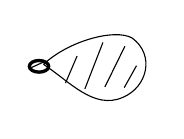
\begin{tikzpicture}[x=.82cm,y=.82cm]
\draw (-.72,.08) .. controls (-.34,.44) and (.38,.64) .. (.65,.49)
  .. controls (1.01,.23) and (.89,-.27) .. (.51,-.43)
  .. controls (.06,-.63) and (-.32,-.18) .. (-.72,.08);
\draw (-.38,-.21) -- (-.20,.21);
\draw (-.08,-.30) -- (.20,.42);
\draw (.23,-.27) -- (.54,.36);
\draw (.53,-.28) -- (.72,.06);
\draw[very thick] (-.79,.05) ellipse (.15 and .09);
\draw (-.91,.03) -- (-.69,.13);
\end{tikzpicture}}\endgroup\par\smallskip Three long strokes and one short stroke in an oval. Dark overlapping marks at the left edge.}
\end{GelfandAdjacentEvidence}
\begin{GelfandAdjacentEvidence}{GELFAND-P000516}{8}

Ex. Wind the 2-dimensional one twice. One gets $RP_{\infty}$.
\SourceFigure{GELFAND-P000516}{exercise-phrase}{The manuscript reads “2-мерную намот. дважды”.}
\end{GelfandAdjacentEvidence}
\begin{GelfandAdjacentEvidence}{GELFAND-P000516}{9}

\SourceFigure{GELFAND-P000516}{exercise-word}{The phrase ends with “дважды” (“twice”).}
\end{GelfandAdjacentEvidence}
\begin{GelfandAdjacentEvidence}{GELFAND-P000516}{10}


\begin{center}— · —\end{center}
Let $M$ — a category that is either abelian or a full subcat. of an abelian cat., closed under extensions. Suppose the isom. classes of objects form a set. Then it is equivalent to a small category.
\uwave{Category \mbox{$QM$}.}\quad
$\underline{\operatorname{Ob}(QM)=\operatorname{Ob}(M)}$.

\[
\operatorname{Hom}_{QM}(X',X'')\ \Rightarrow\ \text{diagrams}
\]
\SourceFigure{GELFAND-P000516}{q-span}{%
\begingroup\color{black}\GelfandFitDiagram{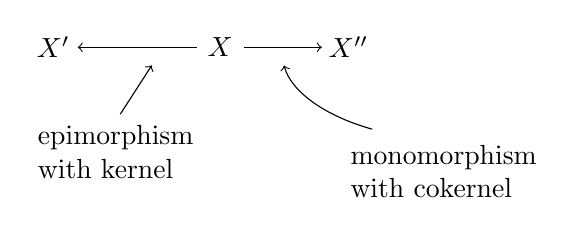
\begin{tikzpicture}
\node at (0,0) {$X'$};
\node at (2.12,0) {$X$};
\node at (3.75,0) {$X''$};
\draw[<-] (.31,0) -- (1.82,0);
\draw[->] (2.42,0) -- (3.41,0);
\draw[->] (.85,-.85) -- (1.25,-.23);
\draw[->] (4.05,-1.04) .. controls (3.41,-.86) and (3.01,-.54) .. (2.93,-.23);
\node[align=left,anchor=north west] at (-.32,-.87) {epimorphism\\with kernel};
\node[align=left,anchor=north west] at (3.65,-1.12) {monomorphism\\with cokernel};
\end{tikzpicture}}\endgroup}
\end{GelfandAdjacentEvidence}
\begin{GelfandAdjacentEvidence}{GELFAND-P000516}{11}


This is a category.

\uline{Definition.}
\SourceFigure{GELFAND-P000516}{k-definition}{%
\begingroup\color{black}\GelfandFitDiagram{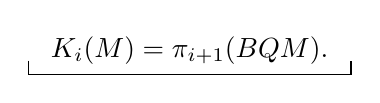
\begin{tikzpicture}
\node[inner xsep=8pt] (formula) {$K_i(M)=\pi_{i+1}(BQM).$};
\draw ([yshift=5pt]formula.south west) |- (formula.south east) -- ++(0,5pt);
\end{tikzpicture}}\endgroup}
\end{GelfandAdjacentEvidence}



\Needspace{7\baselineskip}
\begin{GelfandAdjacentEvidence}{GELFAND-P000517}{1}
\SourcePage{GELFAND-P000517}{unlabelled}
\uline{Continuation of Fuchs’s talk} (following Marchenko).

\uwave{Example of realization}

$S_q$ consists of $q+2$ elements. Interpret it as the set of aff. maps from
$\Delta^q$ into the segment $\Delta^1$, compatible with the ordering of the vertices of $\Delta^q$ and $\Delta^1$.

The morphisms $S_{q-1}\leftarrow S_q\to S_{q+1}$ are def. as for the singular simplices of the space
$I=\Delta^1$ [inserted above the line: (restriction to affine maps)], i.e. by composition with an embedding and restrictions.
\SourceFigure{GELFAND-P000517}{affine-insertion}{The circled insertion “restriction to affine maps” points to the place after the formula.}
\end{GelfandAdjacentEvidence}
\begin{GelfandAdjacentEvidence}{GELFAND-P000517}{2}


Nondegenerate simplices — 2 0-dimensional $*\to I$ and 1 1-dimensional one.

$S_q\times S_q$\qquad when is an element of $S_q\times S_q$ nondeg.?

Elem. — a pair $(\varphi,\psi)$, it is nondeg. when there are no 2 vertices in $\Delta^q$,
mapped by $\varphi$ and $\psi$ [crossed out:
\Incomplete{GELFAND-P000517}{cancelled-sign}{The reading of the crossed-out sign is unresolved.}
\end{GelfandAdjacentEvidence}
\begin{GelfandAdjacentEvidence}{GELFAND-P000517}{3}
]
into one [crossed out:
\Incomplete{GELFAND-P000517}{cancelled-word}{The reading of the crossed-out word is unresolved.}
\end{GelfandAdjacentEvidence}
\begin{GelfandAdjacentEvidence}{GELFAND-P000517}{4}
] vertex.

\[
S_0\times S_0\quad\text{— 4 elems.}\qquad *\to(0,0),(0,1),(1,0),(1,1)
\]
\[
\begin{gathered}
S_1\times S_1\qquad
\binom{1}{0}\to
\begin{matrix}\varphi&\psi\\0&0\\0&1\end{matrix}
\qquad
\left(\begin{matrix}0&1\\0&1\end{matrix}\ \text{degenerate}\right)\\
\begin{pmatrix}0&0\\1&1\end{pmatrix}
\begin{pmatrix}0&0\\1&0\end{pmatrix}
\begin{pmatrix}0&1\\1&1\end{pmatrix}
\begin{pmatrix}1&0\\1&1\end{pmatrix}
\end{gathered}
\]
\Unclear{GELFAND-P000517}{array-cancellation}{A stroke resembling a closing parenthesis is crossed out after the second column, before “degenerate”.}
\end{GelfandAdjacentEvidence}
\begin{GelfandAdjacentEvidence}{GELFAND-P000517}{5}

\[
S_2\times S_2\qquad \Delta\to
\begin{matrix}0&0&0&0\\1&0&0&1\\1&1&1&1\end{matrix}
\]
\SourceFigure{GELFAND-P000517}{double-array}{The manuscript has four columns with no dividers.}
\end{GelfandAdjacentEvidence}
\begin{GelfandAdjacentEvidence}{GELFAND-P000517}{6}


Realization of $S\times S$.
\SourceFigure{GELFAND-P000517}{realization-square}{%
\begingroup\color{black}\GelfandFitDiagram{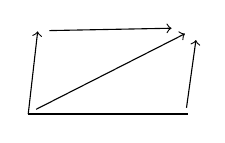
\begin{tikzpicture}
\draw[->] (0,0) -- (.12,1.05);
\draw[->] (.27,1.06) -- (1.82,1.09);
\draw[->] (2.01,.08) -- (2.13,.94);
\draw[->] (.10,.06) -- (1.99,1.02);
\draw (0,0) -- (2.03,0);
\end{tikzpicture}}\endgroup\par\smallskip Strokes overlap at the right end of the lower side. Its direction is unresolved.}
\end{GelfandAdjacentEvidence}
\begin{GelfandAdjacentEvidence}{GELFAND-P000517}{7}


\uline{Classif. space of a category.}

$C$ — a small cat., $NC$ — the nerve of the category

$(NC)_q\ (=S_q)$ — all diagrams in $C$ of the form $X_0\to\ldots\to X_q$

the maps — taking compositions, discarding endpoints and inserting $\mathrm{id}\,X_j$.
\Unclear{GELFAND-P000517}{endpoint-abbreviation}{The Russian abbreviation before “endpoints” is provisionally read “отбрс.”. It could be “отброс.”.}
\end{GelfandAdjacentEvidence}
\begin{GelfandAdjacentEvidence}{GELFAND-P000517}{8}

\Unclear{GELFAND-P000517}{identity-index}{The subscript on $X$ is provisionally set as $j$. It could be a capital $J$.}
\end{GelfandAdjacentEvidence}
\begin{GelfandAdjacentEvidence}{GELFAND-P000517}{9}

\[
BC=\mathrm{Real}\,NC.
\]
The vertices of $BC$ — objects of $C$, 1-dimensional simplices are nonidentity morphisms.
$\Delta$ are stretched over commutative simplices
\SourceFigure{GELFAND-P000517}{commutative-triangle}{%
\begingroup\color{black}\GelfandFitDiagram{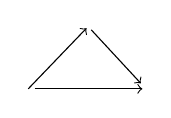
\begin{tikzpicture}
\draw[->] (0,0) -- (.74,.77);
\draw[->] (.80,.75) -- (1.43,.07);
\draw[->] (.08,0) -- (1.45,0);
\end{tikzpicture}}\endgroup}
\end{GelfandAdjacentEvidence}
\begin{GelfandAdjacentEvidence}{GELFAND-P000517}{10}

and so on.

Barycentr. subdiv. of a polyhedron of high deg. is the nerve of some category.
\Unclear{GELFAND-P000517}{subdivision-abbreviation}{The Russian abbreviation is provisionally read “подразд.”. The last letter could be “б”.}
\end{GelfandAdjacentEvidence}


\uline{Properties:}
\[
B(C\times C')\cong BC\times BC'
\]
\[
f:C\rightsquigarrow C'\quad\Rightarrow\quad Bf:BC\to BC'
\]
If there is also $g:C\to C'$ and a nat. map from $f$ to $g$, then
$Bg:BC\to BC'$ is connected to $Bf$ by a canonical homotopy.

Let $\{0,1\}$ — a cat. of 2 objects with one morphism $0\to1$

A morphism of the functors $f$ and $g$ — a functor from $C\times\{0,1\}$ to $C'$.


\Needspace{7\baselineskip}
\begin{GelfandAdjacentEvidence}{GELFAND-P000518}{1}
\SourcePage{GELFAND-P000518}{21}
$F:C\times\{0,1\}\to C'$. At the endpoints $f,g$; morph. $0,1$ — nat. map.

It determines a map, a homotopy connecting $f$ with $g$
\[
BC\times I=B(C\times I)\to BC'.
\]

If $C$ has a terminal or an initial object, then $BC$ is contractible —\\
— it is a cone.

If $f:C\rightsquigarrow C'$ has a left or right adjoint, then $Bf$ — a homotopy equivalence.
\[
BC^{\circ}=BC,\qquad B(C\times C')=BC\times BC'.
\]

\uline{Analogue of the homotopy sequence of a fibration.}

Let $f:X\to Y$ — a Serre fibration. Then
\[
\begin{aligned}
\ldots\to\pi_q(X,x)\to\pi_q(Y,f(x))
&\to\pi_{q-1}(f^{-1}(f(x),x)\\
&\to\pi_{q-1}(X,x)\to\ldots
\end{aligned}
\]
\SourceFigure{GELFAND-P000518}{fibre-parentheses}{The parentheses follow the manuscript. One closing parenthesis is visible before the comma.}
\end{GelfandAdjacentEvidence}
\begin{GelfandAdjacentEvidence}{GELFAND-P000518}{2}


If $f$ does not satisfy the homotopy lifting axiom, then after replacement by an equivalent map it will satisfy it and we get the sequence. Here is the construction:

Let $\widetilde X=\{(x,s),\ x\in X,\ s:I\to Y,\ s(0)=f(x)\}$.

$\widetilde X\underset{\sim}{\supset}X$. The map $\widetilde f:\widetilde X\to Y$ is constructed as follows:

$\widetilde f(x,s)=s(1),\qquad\widetilde f|_X=f$ but now the homotopy lifting axiom holds.

Because $\widetilde X\simeq X$ we have an exact sequence.
\Unclear{GELFAND-P000518}{homotopy-relation}{The sign between $\widetilde X$ and $X$ is provisionally set as $\simeq$. A wavy stroke crosses a straight one in the manuscript.}
\end{GelfandAdjacentEvidence}
\begin{GelfandAdjacentEvidence}{GELFAND-P000518}{3}

\[
\ldots\to\pi_q(X)\to\pi_q(Y)\to
\pi_{q-1}(\text{homot. fibre})\to\pi_{q-1}(X)\to\ldots
\]

Now let \underline{$g:C\rightsquigarrow C'$}, then we have

$Bg:BC\rightsquigarrow BC'$. We would like to construct a “homotopy fibre” of $Bg$.

This has not been done. There is a surrogate.

The constr. also depends on some object $Y\in\mathrm{Ob}\,C'$.

Def. the category $Y\backslash g$. $\mathrm{Ob}(Y\backslash g)$ — the pairs $(X,u)$, where
\[
X\in\mathrm{Ob}\,C,\qquad u\in\mathrm{Mor}_{C'}(Y,g(x)).
\]

A morphism $(X,u)$ to $(X',u')$ — a morphism $\varphi:X\to X'$,
compat. with $u$ and $u'$. There is a nat. map
\[
B(Y\backslash g)\to\text{homot. fibre }Bg:BC\to BC'
\]
\SourceFigure{GELFAND-P000518}{object-case}{The argument of $g(x)$ shows a lowercase $x$. The letters in the pairs in the description of the morphism read as uppercase $X$ and $X'$.}
\end{GelfandAdjacentEvidence}


\uline{Theorem}. Let the functor $g$ be such that

$\forall v\in\mathrm{Mor}_{C'}(Y,Y')$ the resulting map is
$Y'\backslash g\overset{v\backslash g}{\longrightarrow}Y\backslash g$
and $B(v\backslash g):B(Y'\backslash g)\to B(Y\backslash g)$ is a homot. equivalence
(which in general is false). Then $B(Y\backslash g)$ — homot. fibre
$BC\overset{Bg}{\rightsquigarrow}BC'$.


\Needspace{7\baselineskip}
\begin{GelfandAdjacentEvidence}{GELFAND-P000519}{1}
\SourcePage{GELFAND-P000519}{unlabelled}
Construct the map $B(Y\backslash g)$ — homot. fibre of $Bg$.

If there is $(X_0,u_0)\leftarrow\cdots\leftarrow(X_\tau,u_\tau)$
(a simplex of $B(Y\backslash g)$)
then there is also $X_0\leftarrow\cdots\leftarrow X_\tau$
and one only needs to know $Y\to g(X_\tau)$ (from it all the following are recovered: $u_j$
\SourceFigure{GELFAND-P000519}{unclosed-parenthesis}{The manuscript has no closing parenthesis after this line.}
\end{GelfandAdjacentEvidence}
\begin{GelfandAdjacentEvidence}{GELFAND-P000519}{2}


$X_0\leftarrow\cdots\leftarrow X_\tau$ — a simplex of $BC$ of dimension $\tau$.
Together with $u_\tau$ it defines a simplex
\[
g(X_0)\leftarrow\cdots\leftarrow g(X_\tau)\overset{u}{\leftarrow}Y
\]
in $BC'$.
\Unclear{GELFAND-P000519}{simplex-index}{The index is provisionally set as $\tau$. The same letter is used for the dimensions.}
\end{GelfandAdjacentEvidence}
\begin{GelfandAdjacentEvidence}{GELFAND-P000519}{3}


Thus, from a simplex in $B(Y\backslash g)$ we have defined 2 simplices, in $BC$ and in $BC'$
of dimensions $\tau$ and $\tau+1$ resp..
A simplex from $B(Y\backslash g)$ is mapped as follows: the point of the space $BC$
corresponding to that point (in barycentric coord.) and the straight path in the simplex of $BC'$, connecting $Bg$ of this point to $Y$:
\SourceFigure{GELFAND-P000519}{simplex-sketch}{%
\begingroup\color{black}\GelfandFitDiagram{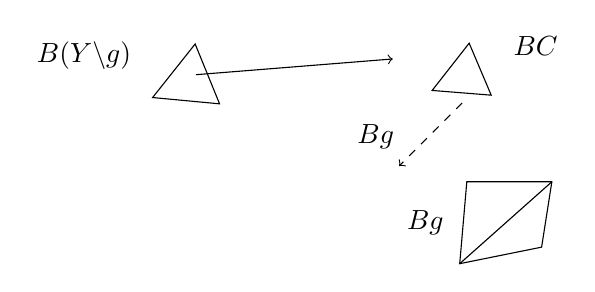
\begin{tikzpicture}[x=1cm,y=1cm]
\node[anchor=east] at (-.15,1.08) {$B(Y\backslash g)$};
\draw (0,.55) -- (.54,1.23) -- (.85,.47) -- cycle;
\draw[->] (.55,.84) -- (3.05,1.04);
\draw (3.55,.64) -- (4.02,1.24) -- (4.30,.58) -- cycle;
\node[anchor=west] at (4.46,1.2) {$BC$};
\draw[dashed,->] (3.93,.48) -- (3.13,-.32);
\node[anchor=east] at (3.19,.05) {$Bg$};
\draw (3.90,-1.56) -- (3.99,-.52) -- (5.07,-.52) -- (4.94,-1.35) -- cycle;
\draw (3.90,-1.56) -- (5.07,-.52);
\node[anchor=east] at (3.82,-1.04) {$Bg$};
\end{tikzpicture}}\endgroup\par\smallskip Overlapping strokes follow $Bg$ on the left side of the quadrilateral. Their reading is unresolved.}
\end{GelfandAdjacentEvidence}
\begin{GelfandAdjacentEvidence}{GELFAND-P000519}{4}


This is a homot. equiv. $\forall v$ iff the conditions of the theorem hold.
\SourceFigure{GELFAND-P000519}{sketch-quantifier}{The beginning of the second line to the right of the sketch reads $\forall v$.}
\end{GelfandAdjacentEvidence}
\begin{GelfandAdjacentEvidence}{GELFAND-P000519}{5}


\uline{Remark by Fuchs}: probably $Y\backslash g$ should be def. as the inverse limit over the spectrum of all
\underline{$Y\backslash g$} \uline{with d}ifferent $Y$.

\uuline{Mishchenko.} (\uwave{Representations according to Mishchenko})

$\Lambda$ — a ring with involution, $H$ — a Hilbert space and 2 reprs.
$T_1$ and $T_2$ of the ring $\Lambda$ into the algebra of bounded op. in $H$, $F$ — a Fredholm operator in $H$ and let
\[
\forall\lambda\in\Lambda\qquad FT_1(\lambda)-T_2(\lambda)F\in\operatorname{Comp}(H)
\]
This system $\{T_1,T_2,F\}$ is called a Fredholm repr. of $\Lambda$.

Atiyah considered $\Lambda=C(M)$, $M$ — a manifold (symposium in Tokyo).
\SourceFigure{GELFAND-P000519}{atiyah-parenthesis}{The parenthetical in the manuscript reads “symposium in Tokyo”.}
\end{GelfandAdjacentEvidence}
\begin{GelfandAdjacentEvidence}{GELFAND-P000519}{6}


\uline{Constr. with these rep}resentations

1) Atiyah (1970) $\Lambda=C(M)$\qquad
$\forall$ repr., assign $\operatorname{index}T\in K_0(M)$

2) $\Lambda=\mathbb Z[\pi]\quad\Rightarrow\quad\forall$ repr., construct
$\xi_T\in K^0(B\pi)$.

3) $\Lambda$ — arbitrary,\qquad
$A=(a_{ij})$ — a quadr. form on $\Lambda^n$\quad $(a_{ij}\in\Lambda)$
\[
A^*=A,\quad\exists A^{-1}\quad\Rightarrow\quad
\text{Construct }\operatorname{sign}_T A\in\mathbb Z.
\]

\Incomplete{GELFAND-P000519}{cancelled-number}{Crossed-out number before “1)”. Possibly “4)”.}
\end{GelfandAdjacentEvidence}
\begin{GelfandAdjacentEvidence}{GELFAND-P000519}{7}

1) $\Lambda=C(M)$, $T$ — a Fredh. repr. of $\Lambda$ in $H$,\quad $T=(T_1,T_2,F)$.

$H_i$ — modules over $\Lambda$.\qquad $\operatorname{ind}F$ — a number.
Let $\eta$ — a bundle,
$\Gamma(\eta)$ — a proj. module over $C(M)$. Consider
\end{GelfandAdjacentEvidence}



\Needspace{7\baselineskip}
\begin{GelfandAdjacentEvidence}{GELFAND-P000520}{1}
\SourcePage{GELFAND-P000520}{22}
\[
H_1\otimes_{C(M)}\Gamma(\eta)
\overset{F\otimes 1_\eta}{\longrightarrow}
H_2\otimes_{C(M)}\Gamma(\eta)
\]
\[
\operatorname{ind}(F\otimes1_\eta):K^0(M)\to\mathbb Z,
\quad\text{i.e. an element of }K_0(M)
\]
This is somewhat crude because $\exists$ elements of finite order in $K^0(M)$.

More precisely: $T$ determines $\operatorname{index}_T:K^0(M\times Y)\to K^0(Y)$;\quad $\forall Y$.
This is already an element of $K_0(M)$.

If $\sigma(A)\in K^0(T^*M)$,\quad $A:H\to H$,\quad since $[f,A]$ —
compact, there is
\Incomplete{GELFAND-P000520}{cancelled-before-index}{The short crossed-out group of signs before “index” cannot be read.}
\end{GelfandAdjacentEvidence}
\begin{GelfandAdjacentEvidence}{GELFAND-P000520}{2}

$\operatorname{index}(A)\in K_0(M)$.
\Unclear{GELFAND-P000520}{commutator-connector}{The stroke after the commutator has been retraced. It is provisionally set as a dash.}
\end{GelfandAdjacentEvidence}
\begin{GelfandAdjacentEvidence}{GELFAND-P000520}{3}

Thus these elems. are Poincaré dual to one another
$K^0(T^*M)\underset{\mathcal D}{\sim}K_0(M)$.
Then $\operatorname{index}A=\mathcal D(\sigma(A))$

(NB one can constr. the \uline{direct} image of $A$)

2) $\pi$ — an arbitrary discr. group, $\Lambda=\mathbb Z[\pi]$ — its group ring, $B_\pi$ —\\
— the classif. space. $T$ — a Fredh. repr.: $T=(T_1,F,T_2)$. We need to constr.
$\xi_T\in K(B_\pi)$.

$K(B_\pi)$ is understood as $[B_\pi,BU]$, but $BU\simeq\mathcal F$ (Fredh. op. [inserted below: in $\ell^2$])
\SourceFigure{GELFAND-P000520}{ell-squared-insertion}{“In $\ell^2$” is written below “Fredh. op.”.}
\end{GelfandAdjacentEvidence}
\begin{GelfandAdjacentEvidence}{GELFAND-P000520}{4}

\[
B_\pi\ni x\to\Phi_x\in\mathcal F.
\]
Let. $\varphi_x:H_1\to H_2$ where $F$ from $T$ acted,
$\widetilde B_\pi$ — the universal cover of $B_\pi$, on which there acts $\pi$.
Take $\widetilde B_\pi\times H_i$ with $\pi$ acting on $\widetilde B_\pi$
in the standard way, and on $H_i$ via $T_i$.
Let $\widetilde B_\pi$ — a cell complex (even simplicial).

Constr. $\varphi_x:\widetilde B_\pi\times H_1\to\widetilde B_\pi\times H_2$.
Let $[\widetilde B_\pi]^k$ — the $k$-dim. skeleton of $\widetilde B_\pi$.
Choose one $\sigma_i^0\in[\widetilde B_\pi]^0$ in any orbit of the action of
$\pi$ and set $\Phi_{\sigma_i^0}\overset{\mathrm{def}}{=}F$.
\SourceFigure{GELFAND-P000520}{vertex-membership}{The $\in$ sign touches the left bracket of the skeleton.}
\end{GelfandAdjacentEvidence}
\begin{GelfandAdjacentEvidence}{GELFAND-P000520}{5}

We have:

a) equivariance

b) $\forall x,y\in[\widetilde B_\pi]^0\quad\Rightarrow\quad
\varphi_x-\varphi_y\in\operatorname{Comp}$

Extend this to $[\widetilde B_\pi]^1$; by the simplicial action of $\pi$ we can choose one simplex in $\forall$ orbit and extend over the simplex as
$p\varphi_1+q\varphi_2$, $p+q=1$ with equivariance satisfied.
By ind. we obtain the whole family $\varphi_x$. From equivariance we have
\SourceFigure{GELFAND-P000520}{bundle-triangle}{%
\begingroup\color{black}\GelfandFitDiagram{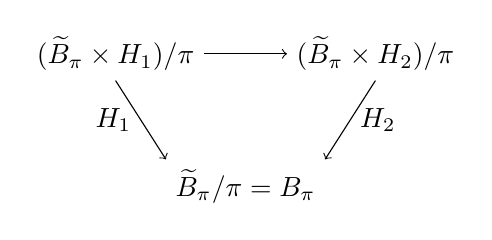
\begin{tikzpicture}[x=1cm,y=1cm]
\node (first) at (-1.65,1.06) {$(\widetilde B_\pi\times H_1)/\pi$};
\node (second) at (1.65,1.06) {$(\widetilde B_\pi\times H_2)/\pi$};
\node (base) at (0,-.62) {$\widetilde B_\pi/\pi=B_\pi$};
\draw[->] (first) -- (second);
\draw[->] (first.south) -- node[left] {$H_1$} (base.north west);
\draw[->] (second.south) -- node[right] {$H_2$} (base.north east);
\end{tikzpicture}}\endgroup}
\end{GelfandAdjacentEvidence}
\begin{GelfandAdjacentEvidence}{GELFAND-P000520}{6}


But by Kuiper $(\widetilde B_\pi\times H_i)/\pi\approx B_\pi\times H_i$.
\SourceFigure{GELFAND-P000520}{kuiper-name}{The manuscript gives the Russian genitive “Кюйпера” for Kuiper.}
\end{GelfandAdjacentEvidence}

After identification we have $B_\pi\times H_1\to B_\pi\times H_2$,
which defines $\varphi_x:H_1\to H_2$.


\Needspace{7\baselineskip}
\begin{GelfandAdjacentEvidence}{GELFAND-P000521}{1}
\SourcePage{GELFAND-P000521}{unlabelled}
\uuline{15/\mbox{$\overline{\underline{X}}$}-73}\qquad \uline{Gelfand’s seminar.}

\uuline{Rudakov.}\qquad
\uwave{On representations of infinite-dimensional Lie algebras.}

Consider $W_n$ — the Lie alg. of form. vector fields
([inserted below: cont.] deriv. of the ring $k[[x_1,\ldots,x_n]]$).
\SourceFigure{GELFAND-P000521}{continuous-insertion}{The circled “cont.” is inserted from below before “deriv.”.}
\end{GelfandAdjacentEvidence}
\begin{GelfandAdjacentEvidence}{GELFAND-P000521}{2}

\[
\left(\sum_{i=1}^{n}a_i(x_1,\ldots,x_n)\frac{\partial}{\partial x_i}\right)
\]
\[
W_n=\mathcal L\supset \text{[crossed out]}\;M\supset M'.
\]
\Unclear{GELFAND-P000521}{upper-chain-cancel}{Lower loops are visible under the crossing out before $M$. This could also be $M$.}
\end{GelfandAdjacentEvidence}
\begin{GelfandAdjacentEvidence}{GELFAND-P000521}{3}

[under $M$: subalg.]
\Incomplete{GELFAND-P000521}{upper-subalgebra-cancel}{The crossed-out words under “subalg.” cannot be read.}
\end{GelfandAdjacentEvidence}
\begin{GelfandAdjacentEvidence}{GELFAND-P000521}{4}

[under $M'$:] an ideal of finite codim. in $M$.

Suppose we are given a repr. of 
\[
M/M'\longrightarrow\text{repr. of }M
\underset{\text{induc.}}{\longrightarrow}\text{representation of }\mathcal L.
\]

\uline{Thm.}: all irred. reprs. of $W_n$ are obtained this way, with finitely many exceptions.

Spaces \uwave{countable-dimensional} discrete (without top.). $E$

[under «countable-dimensional»: (vect. spaces)]

Repr. $\varrho:\mathcal L\longrightarrow\operatorname{Aut}E$, with
\[
x\in E,\ \exists V\subset\mathcal L\qquad \varrho(v)x=0.
\qquad\text{(loc. const. functions).}
\]
[under $V$: nbhd. of $0$]
\SourceFigure{GELFAND-P000521}{representation-argument}{The argument of $\varrho$ is a lowercase $v$. The condition on the left uses a capital $V$.}
\end{GelfandAdjacentEvidence}
\begin{GelfandAdjacentEvidence}{GELFAND-P000521}{5}


Filtrations of nbhds. of zero
\[
\mathcal L=\mathcal L_{-1}\supset\mathcal L_0\supset\ldots
\supset\mathcal L_k\supset\ldots
\]
\[
\mathcal L_k=\left\{\sum a_i\frac{\partial}{\partial x_i}\
\text{[crossed out]},\ \text{deg. }a_i\geqslant k+1\right\}.
\]
\Incomplete{GELFAND-P000521}{filtration-cancel}{The crossed-out notation between the derivative and the comma cannot be read.}
\end{GelfandAdjacentEvidence}
\begin{GelfandAdjacentEvidence}{GELFAND-P000521}{6}


\uline{Assertion}: consider cont. reprs. of $\mathcal L_0/\mathcal L_k$
and irred. reprs. (and inducing representations).

\uwave{Exceptions:} in the \uline{dual spaces to} spaces of closed forms

Suppose there is a repr. of the alg. $\mathcal L$.
\[
x\in E;\quad p(x)=\{\min p:\mathcal L_p x=0\}
\]
($\exists$ there a bounded cont. repr.?).

Consider
\[
\bar p(E)=\min_{\substack{x\in E,\ x\ne0}}p(x).
\]
\[
E_0=\{x\in E,\ p(x)=\bar p(E)\}\text{ — }\mathcal L_0\text{-submodule}.
\]
If $\bar p(E)>1$, then the repr. is induced: $E=\operatorname{Ind}(E_0)$
\Unclear{GELFAND-P000521}{induction-bound}{The digit is retraced. The bottom stroke resembles the base of a $1$. The overlapping strokes make this reading provisional.}
\end{GelfandAdjacentEvidence}


\begin{center}— · —\end{center}
\uline{Exceptions}:
\[
\Omega^p\text{ — form. forms of deg. }p,\qquad
d\Omega^p\text{ — exact forms,}
\]
\[
(d\Omega^p)^*\text{ — the dual space (with the natural topology)}
\]
\begin{center}— · —\end{center}
There are corresponding results for Hamiltonian ones as well.
\begin{center}— · —\end{center}


\Needspace{7\baselineskip}
\begin{GelfandAdjacentEvidence}{GELFAND-P000522}{1}
\SourcePage{GELFAND-P000522}{23}
\uline{Kirillov.}\qquad \uline{A similar result about the group}

Unproved, but well known

$M$ — a manifold, $\operatorname{Diff}M$ — the group of diffeomorphisms.
\Unclear{GELFAND-P000522}{manifold-abbreviation}{The Russian abbreviation is “мн-зие”, probably short for “manifold”.}
\end{GelfandAdjacentEvidence}
\begin{GelfandAdjacentEvidence}{GELFAND-P000522}{2}


describe those reprs. that have finite funct. dimension.
\[
\operatorname{Diff}M\supset H_{x_1,\ldots,x_n}
\]
[under $H_{x_1,\ldots,x_n}$:] keeps fixed $x_1,\ldots,x_n$.

Consider cont. reprs. of $H/H_0$ and induce.

[on the right:] $H_0$ preserves infin. nbhds. of order $n$.

\uuline{Fuchs.} (continuation).

$f:C\longrightarrow C'$ a functor

[under $C$, $C'$:] small cats.
\[
Y\in\operatorname{Ob}C',\qquad Y\backslash f
\]
\[
\operatorname{Ob}(Y\backslash f)=
\{(X,u),\ X\in\operatorname{Ob}C,\ u:Y\longrightarrow f(X)\}.
\]
\[
v:Y\longrightarrow Y'\quad\rightsquigarrow\quad
v\backslash f:Y'\backslash f\longrightarrow Y\backslash f
\]
$\exists$ a nat. map
\[
B(Y\backslash f)\longrightarrow
\text{homot. fibre of the map }Bf:BC\longrightarrow BC'
\]
over the point $Y\in BC'$.

\[
\longleftarrow\ \cdot\ \longrightarrow
\]
\uuline{new cat.} of pairs $(X,u)$, where $X\in\operatorname{Ob}C$,
$u:f(X)\longrightarrow Y$
\SourceFigure{GELFAND-P000522}{dual-comma-box}{%
\begingroup\color{black}\GelfandFitDiagram{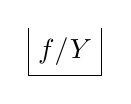
\begin{tikzpicture}
\node (dual) at (0,0) {$f/Y$};
\draw (dual.north west) -- (dual.south west) -- (dual.south east) -- (dual.north east);
\end{tikzpicture}}\endgroup}
\end{GelfandAdjacentEvidence}
\begin{GelfandAdjacentEvidence}{GELFAND-P000522}{3}

another model of the homot. fibre.

The thm. also holds (\uuline{dual})

\uline{Theorem A.} This condition holds if all cats. $Y\backslash f$ are contractible
(i.e.
\Incomplete{GELFAND-P000522}{theorem-a-cancel}{The word after “i.e.” is crossed out. Its reading is unresolved.}
\end{GelfandAdjacentEvidence}
\begin{GelfandAdjacentEvidence}{GELFAND-P000522}{4}

have contractible classif. spaces). Then the conclusion also holds
(in particular, the exact homot. seq.) $\Rightarrow$
$Bf:BC\longrightarrow BC'$ induces isos. of homot. groups.

\begin{center}— · —\end{center}
\uuline{\mbox{$K_i(M)$}}

$M$ — a full subcat. of the ab. cat. $A$, closed under extensions, i.e. from
\[
0\longrightarrow X'\longrightarrow X\longrightarrow X''\longrightarrow0,
\quad X',X''\in\operatorname{Ob}M
\quad\Rightarrow\quad X\in\operatorname{Ob}M.
\]
If a morphism $i:X'\longrightarrow X$ (from $M$) is included in a short exact seq.,
it is called an admissible monomorphism.
\SourceFigure{GELFAND-P000522}{exact-sequence-insertion}{%
\begingroup\color{black}\GelfandFitDiagram{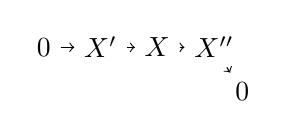
\begin{tikzpicture}[x=.8cm,y=.8cm]
\node (zero) at (0,0) {$0$};
\node (sub) at (.9,0) {$X'$};
\node (middle) at (1.8,0) {$X$};
\node (quotient) at (2.7,0) {$X''$};
\node (end) at (3.15,-.7) {$0$};
\draw[->] (zero) -- (sub);
\draw[->] (sub) -- (middle);
\draw[->] (middle) -- (quotient);
\draw[->] (quotient) -- (end);
\end{tikzpicture}}\endgroup\par\smallskip The final sign in the right-hand insertion is provisionally read as zero.}
\end{GelfandAdjacentEvidence}
\begin{GelfandAdjacentEvidence}{GELFAND-P000522}{5}

(exactness is understood in $A$)

Dual def. if a morph. $p:X\longrightarrow X''$ is included in a short exact seq.,
it is called an adm. epimorphism.

\SourceFigure{GELFAND-P000522}{pullback-diagram}{%
\begingroup\color{black}\GelfandFitDiagram{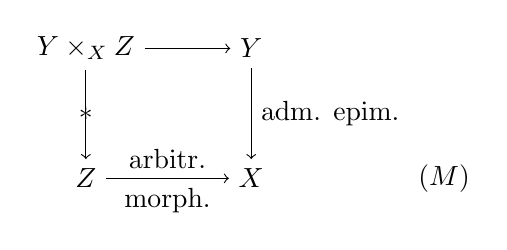
\begin{tikzpicture}[x=1cm,y=1cm]
\node (pullback) at (0,1.65) {$Y\times_X Z$};
\node (upper) at (2.1,1.65) {$Y$};
\node (lower) at (0,0) {$Z$};
\node (base) at (2.1,0) {$X$};
\draw[->] (pullback) -- (upper);
\draw[->] (pullback) -- (lower) node[midway,inner sep=0pt] {$\ast$};
\draw[->] (upper) -- node[right] {adm. epim.} (base);
\draw[->] (lower) -- node[above] {arbitr.} node[below] {morph.} (base);
\node[anchor=west] at (4.1,0) {$(M)$};
\end{tikzpicture}}\endgroup}
\end{GelfandAdjacentEvidence}


Then $Y\times_X Z\in\operatorname{Ob}M$
and $\mathord{\ooalign{\hfil$\downarrow$\hfil\cr\hfil$\scriptstyle\ast$\hfil\cr}}$
— adm. epim..


\Needspace{7\baselineskip}
\begin{GelfandAdjacentEvidence}{GELFAND-P000523}{1}
\SourcePage{GELFAND-P000523}{unlabelled}
From $M$ we construct the cat. $QM$:
\[
\operatorname{Ob}M=\operatorname{Ob}QM.
\]
\[
\operatorname{Mor}_{QM}(X_1,X_2)=
\left\{X_1\overset{\text{a.e.}}{\longleftarrow}X
\overset{\text{a.m.}}{\longrightarrow}X_2\right\}.
\]
Def. equivalence in the obvious way.

([crossed out] $X_1$ — an admiss. subquotient of $X_2$)
\Incomplete{GELFAND-P000523}{subquotient-cancel}{The crossed-out entry before $X_1$ cannot be read.}
\end{GelfandAdjacentEvidence}
\begin{GelfandAdjacentEvidence}{GELFAND-P000523}{2}


\uwave{Def. of composition:}
\SourceFigure{GELFAND-P000523}{composition-corrections}{%
\begingroup\color{black}\GelfandFitDiagram{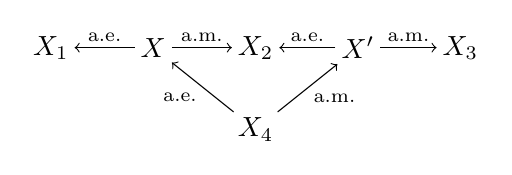
\begin{tikzpicture}[x=1.3cm,y=1cm,every node/.style={inner sep=2pt}]
\node (one) at (0,0) {$X_1$};
\node (left) at (1,0) {$X$};
\node (two) at (2,0) {$X_2$};
\node (right) at (3,0) {$X'$};
\node (three) at (4,0) {$X_3$};
\node (pb) at (2,-1.04) {$X_4$};
\draw[->] (left) -- node[above] {\scriptsize a.e.} (one);
\draw[->] (left) -- node[above] {\scriptsize a.m.} (two);
\draw[->] (right) -- node[above] {\scriptsize a.e.} (two);
\draw[->] (right) -- node[above] {\scriptsize a.m.} (three);
\draw[->] (pb) -- node[below left] {\scriptsize a.e.} (left);
\draw[->] (pb) -- node[below right] {\scriptsize a.m.} (right);
\end{tikzpicture}}\endgroup\par\smallskip
$X_4=X\underset{X_2}{\times}X'$.\par\smallskip The subscript $4$ in the lower vertex and the product formula overwrites an earlier sign. The earlier sign is unreadable. A short stroke is visible at the lower end of the left diagonal arrow.}
\end{GelfandAdjacentEvidence}
\begin{GelfandAdjacentEvidence}{GELFAND-P000523}{3}


and one must take
\[
X_1\overset{\text{a.e.}}{\longleftarrow}X_4
\overset{\text{a.m.}}{\longrightarrow}X_3.
\]
By definition
\[
K_i(M)=\pi_{i+1}(BQM,0),
\]
where $0$ — any of the zero objects of the category $M$.

Isom. classes of objects of $M$ must form a set.

\Incomplete{GELFAND-P000523}{particular-case-cancel}{The crossed-out entry before “Special case” cannot be read.}
\end{GelfandAdjacentEvidence}
\begin{GelfandAdjacentEvidence}{GELFAND-P000523}{4}

\uline{Special case:} (the main one).

$A$ — an arbitrary ring, $PA$ — the cat. of finitely generated projective left $A$-modules.
\SourceFigure{GELFAND-P000523}{definition-bracket}{%
\begingroup\color{black}\GelfandFitDiagram{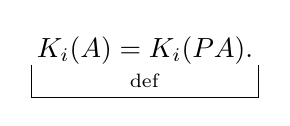
\begin{tikzpicture}
\node (definition) {$K_i(A)=K_i(PA)$.};
\node[font=\scriptsize] at (0,-.38) {$\mathrm{def}$};
\draw (-1.44,-.18) -- (-1.44,-.59) -- (1.44,-.59) -- (1.44,-.18);
\end{tikzpicture}}\endgroup}
\end{GelfandAdjacentEvidence}
\begin{GelfandAdjacentEvidence}{GELFAND-P000523}{5}


\sout{Properties of a certain \mbox{$K$}-functor.}
\Unclear{GELFAND-P000523}{cancelled-k-heading}{The crossed-out abbreviation between “Properties” and K is provisionally read as “некотор.” (“a certain”).}
\end{GelfandAdjacentEvidence}
\begin{GelfandAdjacentEvidence}{GELFAND-P000523}{6}


\[
\underset{\longrightarrow}{\lim}\operatorname{GL}(n,A)=\operatorname{GL}(A).
\]
\[
B\operatorname{GL}(A)
\]
We construct $B_+\operatorname{GL}(A)$ with the properties

1) it is an $H$-space,

2) $B\operatorname{GL}(A)\longrightarrow B_+\operatorname{GL}(A)$

3) the homot. fibre is acyclic

4) surj. map on $\pi_1$.

\[
K_i(A)=\pi_{i+1}(B_+\operatorname{GL}(A))
\text{ — the old def. (Quillen’s)}
\]
\SourceFigure{GELFAND-P000523}{old-index-as-written}{The subscript $i+1$ in this formula follows the manuscript.}
\end{GelfandAdjacentEvidence}
\begin{GelfandAdjacentEvidence}{GELFAND-P000523}{7}


\Unclear{GELFAND-P000523}{apparent-cancel}{A crossed-out entry before “Apparently” may be the beginning of “По-видимому”.}
\end{GelfandAdjacentEvidence}
\begin{GelfandAdjacentEvidence}{GELFAND-P000523}{8}

Apparently $BQPA$ is $B_+\operatorname{GL}(A)$. This is false, but there is a map.
\[
B\operatorname{GL}(A)\longrightarrow BQPA.
\]
Let $S_n$ — a free $A$-mod. with $n$ gens..
\[
S_n\in\operatorname{Ob}(PA)=\operatorname{Ob}(QPA).
\]
Elems. of the group $\operatorname{GL}(n,A)$ — the automs. $S_n\longrightarrow S_n$.
This lets us def. the functor
\[
\operatorname{GL}(n,A)\rightsquigarrow PA.
\]
[under $\operatorname{GL}(n,A)$:] corr. cat. (a single obj.)
\[
\text{obj.}\longrightarrow S_n
\]
\SourceFigure{GELFAND-P000523}{pa-vertical-note}{$\Vert$\quad automs. in $PA$ are morphs. in $QPA$}
\end{GelfandAdjacentEvidence}


Functor $\operatorname{GL}(n,A)\longrightarrow QPA$.


\Needspace{7\baselineskip}
\begin{GelfandAdjacentEvidence}{GELFAND-P000524}{1}
\SourcePage{GELFAND-P000524}{24}
Hence we obtain a map of classif. spaces
\[
B\operatorname{GL}(n,A)\longrightarrow BQPA
\]
It remains to pass to the limit. (They are incompatible).
\[
\begin{aligned}
QPA&\longrightarrow QPA\\
X&\longrightarrow X\oplus A
\end{aligned}
\qquad\text{is a homotopy equivalence.}
\]
Diagr.
\SourceFigure{GELFAND-P000524}{stabilization-square}{%
\begingroup\color{black}\GelfandFitDiagram{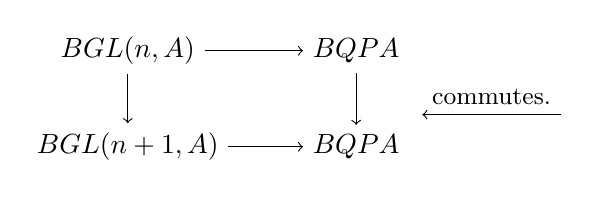
\begin{tikzpicture}[x=1cm,y=1cm]
\node (a) at (0,1.22) {$B\operatorname{GL}(n,A)$};
\node (b) at (2.9,1.22) {$BQPA$};
\node (c) at (0,0) {$B\operatorname{GL}(n+1,A)$};
\node (d) at (2.9,0) {$BQPA$};
\draw[->] (a) -- (b);
\draw[->] (c) -- (d);
\draw[->] (a) -- (c);
\draw[->] (b) -- (d);
\node (commutes) at (4.62,.63) {\small commutes.};
\draw[<-] (commutes.south west) -- (commutes.south east);
\end{tikzpicture}}\endgroup}
\end{GelfandAdjacentEvidence}

and hence the limit and the map
\[
B\operatorname{GL}(A)\longrightarrow BQPA
\]


\Needspace{7\baselineskip}
\begin{GelfandAdjacentEvidence}{GELFAND-P000525}{1}
\SourcePage{GELFAND-P000525}{unlabelled}
\uline{22.10.73}\qquad\uline{Gelfand’s seminar.}

\Incomplete{GELFAND-P000525}{speaker-cancellation}{The crossed-out entry before “Gelfand” cannot be read.}
\end{GelfandAdjacentEvidence}
\begin{GelfandAdjacentEvidence}{GELFAND-P000525}{2}

\uline{Gelfand.} \uwave{Publicizing work on nonlin. scattering theory.} (Straus)
\SourceFigure{GELFAND-P000525}{straus-spelling}{The surname in parentheses is written “Straus”.}
\end{GelfandAdjacentEvidence}
\begin{GelfandAdjacentEvidence}{GELFAND-P000525}{3}

\[
U(t)U(s)=U(t+s),
\]
Relation for $U(t)f$ as $t\longrightarrow\pm\infty$

Typical features: $E(U(t)f)=E(f)$; $E$ — some functional

$\exists$ a simpler group $U_0(t)$, such that
\[
E\bigl(U(t)f-U_0(t)f_{\pm}\bigr)\underset{t\to\pm\infty}{\longrightarrow}0
\qquad(\exists f_{\pm})
\]
$S$ — the relation between $f_+$ and $f_-$.

Examples: wave eq.
\[
u_{tt}-\Delta u+u+|u|^2u=0;
\]
\Unclear{GELFAND-P000525}{wave-sign}{The sign before the Laplacian is retraced. The horizontal stroke supports a provisional minus.}
\end{GelfandAdjacentEvidence}
\begin{GelfandAdjacentEvidence}{GELFAND-P000525}{4}

\SourceFigure{GELFAND-P000525}{kdv-time-index}{%
\begingroup\color{black}\GelfandFitDiagram{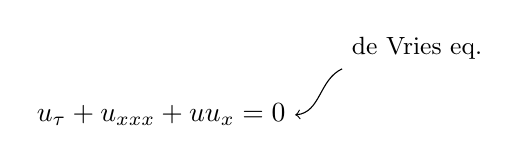
\begin{tikzpicture}[x=1cm,y=1cm]
\node (equation) at (0,0) {$u_\tau+u_{xxx}+uu_x=0$};
\node (label) at (3.25,.85) {\small de Vries eq.};
\draw[->] (label.south west) to[out=205,in=5] (equation.east);
\end{tikzpicture}}\endgroup\par\smallskip The first subscript is provisionally set as $\tau$ from its shape. It differs from the $tt$ on the line above.}
\end{GelfandAdjacentEvidence}
\begin{GelfandAdjacentEvidence}{GELFAND-P000525}{5}

\begin{center}— $\bullet$ —\end{center}

\uline{Kirillov.}

1. \uwave{Kostant’s work.}

$M$ — a symplectic manifold (a nondeg. closed 2-form is given $\omega$).

$TM$ — a bundle over $M$ with struct. group $\operatorname{Sp}(2n,\mathbb R)$. It is not simply connected.

Topol.
\SourceFigure{GELFAND-P000525}{covering-diagram}{%
\begingroup\color{black}\GelfandFitDiagram{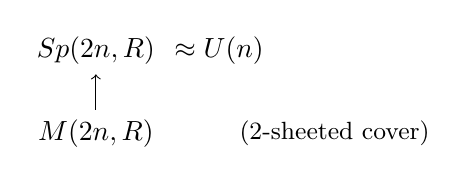
\begin{tikzpicture}[x=1cm,y=1cm]
\node (sp) at (0,1.05) {$\operatorname{Sp}(2n,\mathbb R)$};
\node[anchor=west] at (sp.east) {$\approx U(n)$};
\node (cover) at (0,0) {$M(2n,\mathbb R)$};
\node[anchor=west] at (1.7,0) {\small (2-sheeted cover)};
\draw[->] (cover) -- (sp);
\end{tikzpicture}}\endgroup}
\end{GelfandAdjacentEvidence}
\begin{GelfandAdjacentEvidence}{GELFAND-P000525}{6}

Sometimes the struct. group lifts to
\Incomplete{GELFAND-P000525}{covering-cancellation}{The crossed-out sign before $M(2n,\mathbb R)$ cannot be read.}
\end{GelfandAdjacentEvidence}
\begin{GelfandAdjacentEvidence}{GELFAND-P000525}{7}

$M(2n,\mathbb R)$.

Then on $M$ one constructs a spinor bundle (if $C_1$ is divisible by 2).

$M$ has a special
\Incomplete{GELFAND-P000525}{representation-cancellation}{The crossed-out word before “repr. $T$” cannot be read.}
\end{GelfandAdjacentEvidence}
\begin{GelfandAdjacentEvidence}{GELFAND-P000525}{8}

repr. $T$, called the spinor repr. (or the Weyl repr.)

Alg. $\{p_1,\ldots,p_n,q_1,\ldots,q_n\}$ and the rel.
\[
p_iq_j-q_jp_i=\delta_{ij}
\]
\SourceFigure{GELFAND-P000525}{algebra-abbreviation}{The abbreviation at the start of the line reads “Ал.”.}
\end{GelfandAdjacentEvidence}

(if $+$, then the spin repr. of the orthog. group).

$\operatorname{Sp}(2n,\mathbb R)$ linearly changes $p$ and $q$.

Realiz.
$p_i\longrightarrow\frac{\partial}{\partial x_i}$,
$q_i\longrightarrow x_i$ in $L^2(\mathbb R^n)$.

Automs. of the alg. $\Longrightarrow$ automs. of the alg. of bounded operators.
But they are all inner: $A\longrightarrow UAU^{-1}$
($U$ up to a factor) $\Rightarrow$ a projective representation.
The factors reduce to $\pm1$.
The repr. becomes single-valued on the 2-sheeted cover.


\Needspace{7\baselineskip}
\begin{GelfandAdjacentEvidence}{GELFAND-P000526}{1}
\SourcePage{GELFAND-P000526}{28}
2. \uwave{[crossed out] \mbox{$p$}-adic measures}.
\Incomplete{GELFAND-P000526}{title-cancellation}{The crossed-out part of the heading cannot be read.}
\end{GelfandAdjacentEvidence}
\begin{GelfandAdjacentEvidence}{GELFAND-P000526}{2}


$p$-adic measures; $\mathbb Z_p$ — integers;
\Incomplete{GELFAND-P000526}{integers-cancellation}{The crossed-out entry after “integers” cannot be read.}
\end{GelfandAdjacentEvidence}
\begin{GelfandAdjacentEvidence}{GELFAND-P000526}{3}


Consider $C(\mathbb Z_p,K)$, $K$ — a finite ext. of the $p$-adic field

(cont. funcs. with values in $K$)
\[
\operatorname{Hom}\bigl(C(\mathbb Z_p,K),\mathbb Q_p\bigr)
=C(\mathbb Z_p,K)'=M(\mathbb Z_p,K)
\]
(measures with $p$-adic values)
\SourceFigure{GELFAND-P000526}{dual-codomain}{The second argument of $\operatorname{Hom}$ reads $\mathbb Q_p$.}
\end{GelfandAdjacentEvidence}
\begin{GelfandAdjacentEvidence}{GELFAND-P000526}{4}


There is a convolution on measures
\SourceFigure{GELFAND-P000526}{convolution-bracket}{%
\begingroup\color{black}\GelfandFitDiagram{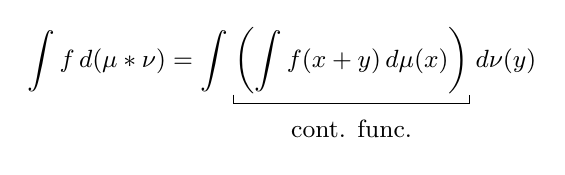
\begin{tikzpicture}
\node[inner sep=0pt,font=\small] (left) at (0,0) {$\displaystyle\int f\,d(\mu*\nu)=\int$};
\node[inner sep=0pt,font=\small,anchor=west] (inner) at ([xshift=2pt]left.east)
 {$\displaystyle\left(\int f(x+y)\,d\mu(x)\right)$};
\node[inner sep=0pt,font=\small,anchor=west] (right) at ([xshift=2pt]inner.east) {$d\nu(y)$};
\draw (inner.south west) -- ++(0,-.11) -| (inner.south east);
\node[font=\small,anchor=north,yshift=-2mm] at (inner.south) {cont. func.};
\end{tikzpicture}}\endgroup}
\end{GelfandAdjacentEvidence}
\begin{GelfandAdjacentEvidence}{GELFAND-P000526}{5}


\uline{Theorem 1.}
\Incomplete{GELFAND-P000526}{theorem-one-cancellation}{The crossed-out entry after “Theorem 1” cannot be read.}
\end{GelfandAdjacentEvidence}
\begin{GelfandAdjacentEvidence}{GELFAND-P000526}{6}

$K$-algebra of measures $M(\mathbb Z_p,K)=K[[T]]$.
\[
\left\|\sum a_kT^k\right\|=\sup_k|a_k|
\qquad\text{(series of finite norm)}
\]
Form. series are obtained from unbounded measures.

\uline{Theorem 2.} Consider $M(\mathbb Z_p^*,K)=(p-1)K[[T]]$.

Unbounded measures are finitely add. on elem. sets (dual to loc. const. funcs.).

\uuline{Proof} of Thm. 1.
\[
\mu\longrightarrow\sum a_kT^k,\qquad
\text{where }a_k=\int_{\mathbb Z_p}\frac{x(x-1)\cdots(x-k+1)}{k!}\,d\mu(x)
\]
\[
\sum a_kT^k=\int_{\mathbb Z_p}(1+T)^x\,d\mu(x).
\]
it follows that convolution of measures $\longrightarrow$ product of series.

\SourceFigure{GELFAND-P000526}{shaded-quadrilateral}{%
\begingroup\color{black}\GelfandFitDiagram{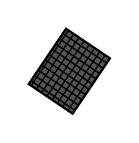
\begin{tikzpicture}[rotate=-34,scale=.73]
\fill[black!67] (0,0) rectangle (.92,1.16);
\foreach \x in {.05,.16,...,.89}
  \draw[line width=.45pt] (\x,0) -- (\x,1.16);
\foreach \y in {.07,.18,...,1.1}
  \draw[line width=.5pt] (0,\y) -- (.92,\y);
\draw[thick] (0,0) rectangle (.92,1.16);
\end{tikzpicture}}\endgroup\par\smallskip A tilted shaded quadrilateral between the formulas. Its purpose is unclear.}
\end{GelfandAdjacentEvidence}
\begin{GelfandAdjacentEvidence}{GELFAND-P000526}{7}

\[
1+T=e^\tau\qquad\text{($\tau$ — form. var.)}
\qquad\int_{\mathbb Z_p}e^{\tau x}\,d\mu(x)=\widetilde{\mu}(\tau)
\]
(rewrite the analysis!)

$\tau$ can be treated as a number.
\[
\tau=\ln(1+T)=T-\frac12T^2+\frac13T^3-\ldots
\]
It is unclear what range of funcs. will result (after substitution one should get a series with integer coeffs.)

\uuline{Example}
([crossed out])
\uwave{(Cartier) as presented by Gelfand}
\Incomplete{GELFAND-P000526}{example-cancellation}{The entry in the first parentheses after “Example” is crossed out and cannot be read.}
\end{GelfandAdjacentEvidence}
\begin{GelfandAdjacentEvidence}{GELFAND-P000526}{8}


Consider
\[
\ln(1-a)=a+\frac{a^2}{2}+\frac{a^3}{3}+\ldots
\qquad\text{and }a=2\in\mathbb Z_2.
\]
\SourceFigure{GELFAND-P000526}{logarithm-signs}{The manuscript has $a$ after the equals sign, followed by plus signs.}
\end{GelfandAdjacentEvidence}
\begin{GelfandAdjacentEvidence}{GELFAND-P000526}{9}

The series converges [inserted below: and equals] $\ln(-1)$.
\SourceFigure{GELFAND-P000526}{log-equality-insertion}{The circled insertion “and equals” points to the line above.}
\end{GelfandAdjacentEvidence}
\begin{GelfandAdjacentEvidence}{GELFAND-P000526}{10}

\[
\ln[(-1)^2]=2\ln(-1)=0\quad\Rightarrow\quad\ln(-1)=0.
\]
hence the series converges to 0
\[
2+\frac{2^2}{2}+\frac{2^3}{3}+\frac{2^4}{4}+\frac{2^5}{5}
+\ldots+\frac{2^n}{n}+\ldots=0
\]
\[
S_n=2+\frac{2^2}{2}+\frac{2^3}{3}+\ldots+\frac{2^n}{n}
\qquad\text{for large $n$ is divisible by }2^k
\]
$2$, $4$, $\dfrac{20}{3}$, $\dfrac{32}{3}$ and so on.
\begin{center}— $\cdot$ —\end{center}

\uline{Theorem.}
\[
\|\mu\|=\sup_k|a_k|\qquad(\approx\text{ Plancherel})
\]
\[
\|\mu\|\underset{\mathrm{def}}{=}\sup_{|f|\leq1}\left|\int f\,d\mu\right|
\]
From the formula $\|\mu\|\geq\sup_k|a_k|$

We need to check
\[
\begin{gathered}
|f|\leq1\quad\Rightarrow\quad f(x)=\sum c_kP_k(x),\qquad |c_k|\leq1,\\
P_k(x)=\frac{x(x-1)\cdots(x-k+1)}{k!}
\end{gathered}
\]
(\uline{Proof}: approx. by polynomials and apply the thm.)
\[
c_k=\sum_{i=0}^k(-1)^{i+k}C_k^if(i)=\Delta^kf(0)
\qquad\text{(Taylor formula)}
\]
\[
\begin{aligned}
X^{\tikz[baseline=(degree.base)]{\node[draw,circle,inner sep=.4pt] (degree) {$\scriptstyle k$};}}
&=x(x-1)\cdots(x-k+1),\\
\Delta X^{\tikz[baseline=(degree.base)]{\node[draw,circle,inner sep=.4pt] (degree) {$\scriptstyle k$};}}
&=kx^{\tikz[baseline=(degree.base)]{\node[inner sep=.5pt] (degree) {$\scriptstyle k-1$};
 \draw (degree.center) ellipse (.22 and .11);}},
\qquad\text{where }\Delta f(x)=f(x+1)-f(x).
\end{aligned}
\]
\Unclear{GELFAND-P000526}{falling-variable}{The first two letters with a circled index are provisionally set as $X$. The letter after the factor $k$ is set as $x$.}
\end{GelfandAdjacentEvidence}



\Needspace{7\baselineskip}
\begin{GelfandAdjacentEvidence}{GELFAND-P000527}{1}
\SourcePage{GELFAND-P000527}{unlabelled}
\[
f(x)=\sum_{k=0}^{\infty}\frac{1}{k!}
X^{\tikz[baseline=(degree.base)]{\node[draw,circle,inner sep=.4pt] (degree) {$\scriptstyle k$};}}
\cdot f^{\tikz[baseline=(degree.base)]{\node[inner sep=.4pt] (degree) {$\scriptstyle(k)$};
  \draw (degree.center) ellipse (.20 and .13);}}(0),
\qquad
\text{where } f^{\tikz[baseline=(degree.base)]{\node[inner sep=.4pt] (degree) {$\scriptstyle(k)$};
  \draw (degree.center) ellipse (.20 and .13);}}(x)=(\Delta^k f)(x)
\]
\SourceFigure{GELFAND-P000527}{series-notation}{The letter with circled $k$ in the first product reads as $X$. Both indices $(k)$ on $f$ are also circled.}
\end{GelfandAdjacentEvidence}
\begin{GelfandAdjacentEvidence}{GELFAND-P000527}{2}


\uline{Assn.}: $\forall$ cont. funcs.
\Incomplete{GELFAND-P000527}{top-cancellation}{The crossed-out word before “series” cannot be read.}
\end{GelfandAdjacentEvidence}
\begin{GelfandAdjacentEvidence}{GELFAND-P000527}{3}

the Maclaurin series converges uniformly, and,
\[
\max|f|=\max|a_k|.
\]
\Unclear{GELFAND-P000527}{modulus-stroke}{There is a thick stroke before $f$ in the manuscript. It is provisionally set as one absolute-value bar.}
\end{GelfandAdjacentEvidence}
\begin{GelfandAdjacentEvidence}{GELFAND-P000527}{4}


\uwave{Next time Kirillov (3 more min.) and Mishchenko.}

\uuline{Fuchs}. (continuation).

$M$ — an add. full subcat. of an abelian category, closed under extensions
\[
QM:\qquad \operatorname{Ob}QM=\operatorname{Ob}M.
\]
\SourceFigure{GELFAND-P000527}{qm-span}{%
\begingroup\color{black}\GelfandFitDiagram{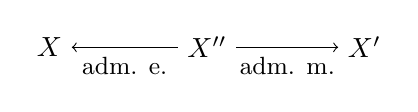
\begin{tikzpicture}[x=1cm,y=1cm]
\node (left) at (0,0) {$X$};
\node (middle) at (2,0) {$X''$};
\node (right) at (4,0) {$X'$};
\draw[->] (middle) -- node[below] {\small adm. e.} (left);
\draw[->] (middle) -- node[below] {\small adm. m.} (right);
\end{tikzpicture}}\endgroup}
\end{GelfandAdjacentEvidence}
\begin{GelfandAdjacentEvidence}{GELFAND-P000527}{5}

\[
\pi_i(BQM)
\]
$BQM$ is homol. equiv. to $B\operatorname{GL}(\infty,A)$

\uline{Def.} \uline{Grothendieck gr. of the category \mbox{$M$}.}
\uline{Gens.} — \uwave{the objects of \mbox{$M$}}, rels.
\[
0\to X'\to X\to X''\to0,\qquad\Rightarrow\quad X=X'+X''
\]
The gr. is commutative, since $\exists\ X=X'\oplus X''$.

\uuline{Theorem:}
\[
\underset{\substack{\Vert\\\pi_1(BQM,0)}}{K_0(M)}\cong
\text{Grothendieck gr. of the cat. }M.
\]
Zero-dim. skeleton $=\operatorname{Ob}(M)$

1-dim. skeleton — the morphisms of $QM$

$\forall X$ a loop is def.
\SourceFigure{GELFAND-P000527}{loop-figure}{%
\begingroup\color{black}\GelfandFitDiagram{\begin{tikzpicture}[x=1cm,y=1cm]
\node (zero) at (0,0) {$0$};
\node (x) at (2.15,.83) {$X$};
\draw[->] (zero) to[bend left=30] node[above left] {\small adm. m.} (x);
\draw[->] (x) to[bend left=32] node[below right] {\small $($adm. epi.$)^{-1}$} (zero);
\node at (3.9,.15) {$\zeta_X$.};
\end{tikzpicture}}\endgroup}
\end{GelfandAdjacentEvidence}
\begin{GelfandAdjacentEvidence}{GELFAND-P000527}{6}


If in $M$ there is an exact seq. (short) $0\to X'\to X\to X''\to0$,
then
\[
\zeta_X\sim\zeta_{X'}\cdot\zeta_{X''}.
\]
\Unclear{GELFAND-P000527}{loop-notation}{The letter denoting the loop is provisionally set as $\zeta$.}
\end{GelfandAdjacentEvidence}
\begin{GelfandAdjacentEvidence}{GELFAND-P000527}{7}


\SourceFigure{GELFAND-P000527}{lower-diagram}{%
\begingroup\color{black}\GelfandFitDiagram{\begin{tikzpicture}[x=1cm,y=1cm,every node/.style={inner sep=1.6pt}]
\node (left) at (0,2.38) {$X'$};
\node (middle) at (2.45,2.52) {$X$};
\node (right) at (4.97,2.6) {$X''$};
\node at (2.54,-.04) {$0$};
\draw[->] (left) -- node[above] {\small a.m.} (middle);
\draw[->] (right) -- node[above] {\small a.e.$^{-1}$} (middle);
\draw[black!60,thin] (.24,2.1) -- (1.1,2.53);
\draw[black!60,thin] (.36,1.85) -- (1.66,2.46);
\draw[black!60,thin] (.46,1.63) -- (2.03,2.45);
\draw[black!60,thin] (.76,1.28) -- (2.23,2.02);
\draw[black!60,thin] (1.05,.89) -- (2.08,1.38);
\draw[black!60,thin] (1.23,.59) -- (2.22,1.04);
\draw[black!60,thin] (1.34,.43) -- (2.4,.65);
\draw[black!60,thin] (1.46,.27) -- (2.5,.5);
\draw[->] (1.42,.18) to[out=160,in=265]
  node[pos=.48,left] {\small a.m.} (.46,1.73);
\draw[->] (1.47,.37) to[out=135,in=300]
  node[pos=.64,right] {\small a.e.$^{-1}$} (.71,1.94);
\draw[->] (2.49,.36) to[out=124,in=221]
  node[pos=.45,left] {\small a.m.} (2.39,1.91);
\draw[->] (2.64,.56) to[out=51,in=300]
  node[pos=.65,right] {\small a.e.$^{-1}$} (2.62,1.93);
\draw[->] (3.43,.51) to[out=50,in=194]
  node[pos=.63,above left] {\small a.m.} (4.54,1.5);
\draw[->] (3.53,.28) to[out=18,in=227]
  node[pos=.57,below right] {\small $($a.e.$)^{-1}$} (4.68,1.26);
\end{tikzpicture}}\endgroup\par\smallskip The lower ends of the arcs are left separate as in the sketch. The thin lines represent the diagonal hatching.}
\end{GelfandAdjacentEvidence}

and recall the 2-simplices.

\begin{center}— $\bullet$ —\end{center}


\Needspace{7\baselineskip}
\begin{GelfandAdjacentEvidence}{GELFAND-P000528}{1}
\SourcePage{GELFAND-P000528}{unlabelled}
\uline{29/\mbox{$\overline{\underline{X}}$}-73.}\qquad\uline{Gelfand’s seminar.}

\uuline{A. A. Kirillov.}

There is a symplectic manifold $M$
\SourceFigure{GELFAND-P000528}{upper-sketch}{%
\begingroup\color{black}\GelfandFitDiagram{\begin{tikzpicture}[x=1cm,y=1cm]
\draw (.94,1.64) .. controls (1.74,1.89) and (2.05,1.57) .. (2.64,1.52)
  .. controls (3.17,1.46) and (3.64,1.25) .. (3.67,.78)
  .. controls (3.78,.28) and (3.05,.02) .. (2.46,.13)
  .. controls (1.99,.28) and (1.58,.12) .. (1.13,.12)
  .. controls (.58,.12) and (.02,.34) .. (.08,.73);
\draw[densely dotted] (.08,.73) .. controls (.10,1.20) and (.44,1.53) .. (.94,1.64);
\draw[rotate around={25:(1.13,.91)}] (1.13,.91) ellipse (.33 and .25);
\draw[rotate around={17:(1.65,1.00)}] (1.65,1.00) ellipse (.42 and .32);
\draw[rotate around={18:(2.16,.96)}] (2.16,.96) ellipse (.33 and .25);
\draw (1.97,1.19) .. controls (2.07,1.28) and (2.20,1.32) .. (2.29,1.29);
\end{tikzpicture}}\endgroup}
\end{GelfandAdjacentEvidence}
\begin{GelfandAdjacentEvidence}{GELFAND-P000528}{2}


\SourceFigure{GELFAND-P000528}{covering-map}{%
\begingroup\color{black}\GelfandFitDiagram{\begin{tikzpicture}
\node (sp) at (0,1.0) {$\operatorname{Sp}(2n,\mathbb R)$};
\node (cover) at (0,0) {$M(n,\mathbb R)$};
\node[anchor=west] at (1.47,0) {\small (2-sheeted cover)};
\draw[->] (cover) -- (sp);
\end{tikzpicture}}\endgroup}
\end{GelfandAdjacentEvidence}
\begin{GelfandAdjacentEvidence}{GELFAND-P000528}{3}

loc. we may take
\[
\omega=\sum_{k=1}^n dp_k\wedge dq_k
\]
Transition funcs. (in $TM$) $g_{ij}\in\operatorname{Sp}(2n,\mathbb R)$

Suppose they are in the 2-sheeted cover $M(2n,\mathbb R)$
\SourceFigure{GELFAND-P000528}{covering-notation}{The line reads $M(2n,\mathbb R)$. The diagram above and the insertion below read $M(n,\mathbb R)$.}
\end{GelfandAdjacentEvidence}
\begin{GelfandAdjacentEvidence}{GELFAND-P000528}{4}


\textbf{The spinor representation} [inserted below: $M(n,\mathbb R)$] in Hilb. space
\Incomplete{GELFAND-P000528}{spinor-cancellation}{The crossed-out sign after “space” cannot be read.}
\end{GelfandAdjacentEvidence}
\begin{GelfandAdjacentEvidence}{GELFAND-P000528}{5}

induces a Hilbert bundle $HM$ over $M$
\SourceFigure{GELFAND-P000528}{spinor-insertion}{The circled insertion $M(n,\mathbb R)$ points to “representation”.}
\end{GelfandAdjacentEvidence}
\begin{GelfandAdjacentEvidence}{GELFAND-P000528}{6}

\[
SM\subset HM\subset S'M
\]
\Unclear{GELFAND-P000528}{schwartz-cancellation}{The crossed-out sign before $S'M$ resembles $H$.}
\end{GelfandAdjacentEvidence}
\begin{GelfandAdjacentEvidence}{GELFAND-P000528}{7}

[under $SM$: rapidly decreasing]

Symplectic transf. $\leadsto$ op. in Hilb. space (can. transf. with $p_i,q_i$)

We obtain a projective representation
\[
\underbrace{GM}=TM\oplus\mathbb R\times M
\]
[under the brace:] polyn. of deg. $\leq2$ in $p$ and $q$ (Heisenberg Lie alg.)
\SourceFigure{GELFAND-P000528}{polynomial-degree}{The sign before $2$ reads $\leq$.}
\end{GelfandAdjacentEvidence}
\begin{GelfandAdjacentEvidence}{GELFAND-P000528}{8}


$GM$ acts on $HM$ compat. with the bundle structure.

$RM$, $R_x$ — Lagrangian subspaces in $T_xM$ (max. dim.)

\uline{A. Shnirelman.}\qquad\uline{On Fermi:} equipartition of energy among degrees of freedom.
\[
\ddot x_k=(x_{k-1}+x_{k+1}-2x_k)+\varepsilon(x_{k-1}-x_k)^2
 +\varepsilon(x_{k+1}-x_k)^2
\]
\SourceFigure{GELFAND-P000528}{dynamics-equation}{Both quadratic terms have plus signs in the manuscript.}
\end{GelfandAdjacentEvidence}
\begin{GelfandAdjacentEvidence}{GELFAND-P000528}{9}


\uwave{Solved num. on a computer}

\underline{$k=16$}\qquad after fin. \sout{time} time intervals they examined the Fourier transf..
\Unclear{GELFAND-P000528}{chain-size}{The number $16$ is legible. The retraced letter is provisionally set as $k$.}
\end{GelfandAdjacentEvidence}
\begin{GelfandAdjacentEvidence}{GELFAND-P000528}{10}

\Unclear{GELFAND-P000528}{time-cancellation}{The crossed-out word is provisionally read as “time”.}
\end{GelfandAdjacentEvidence}
\begin{GelfandAdjacentEvidence}{GELFAND-P000528}{11}

Init. cond. — \uuline{\mbox{$\sin$}}\qquad (all the energy in the 1st harm.)

By the estimate $t=10^{-35}$ in this state.
\SourceFigure{GELFAND-P000528}{time-exponent}{The exponent on the line reads $-35$.}
\end{GelfandAdjacentEvidence}
\begin{GelfandAdjacentEvidence}{GELFAND-P000528}{12}


\uline{Calculations:}
\SourceFigure{GELFAND-P000528}{recurrence-plot}{%
\begingroup\color{black}\GelfandFitDiagram{\begin{tikzpicture}[x=.83cm,y=1.05cm,every node/.style={inner sep=1.3pt}]
\draw (-.42,-.02) .. controls (1.6,.13) and (2.7,.06) .. (3.22,.02)
  .. controls (4.6,-.04) and (5.64,-.12) .. (6.36,-.07);
\draw (0,-.39) -- (.04,1.69);
\draw (3.14,-.30) .. controls (3.28,.52) and (3.03,1.01) .. (3.24,1.90);
\draw (6.36,-.05) .. controls (6.30,.56) and (6.52,1.17) .. (6.57,1.92);
\draw[densely dashed,thin] (.04,1.73) .. controls (1.5,1.63) and (2.1,1.79) .. (3.3,1.89);
\draw[densely dashed,thin] (3.67,1.84) -- (6.55,1.85);
\draw[thick] (.04,1.67) .. controls (.56,1.64) and (.90,1.28) .. (1.16,.95)
  .. controls (1.68,.16) and (2.29,.58) .. (2.77,1.27)
  .. controls (2.98,1.59) and (3.13,1.73) .. (3.23,1.72)
  .. controls (3.79,1.68) and (3.92,.33) .. (4.52,.30)
  .. controls (5.30,.14) and (5.28,1.06) .. (6.45,1.35);
\draw (.04,.04) .. controls (.54,.33) and (.56,1.02) .. (1.36,1.16)
  .. controls (1.53,1.20) and (1.41,.65) .. (1.75,.51)
  .. controls (2.15,.15) and (2.08,1.43) .. (2.47,.97)
  .. controls (2.76,.63) and (3.09,.13) .. (3.30,.02);
\draw (.04,.04) .. controls (.83,.21) and (.84,.80) .. (1.50,.93)
  .. controls (1.88,1.04) and (1.76,1.55) .. (2.29,.98)
  .. controls (2.65,.59) and (2.49,.23) .. (3.30,.02);
\draw (.04,.04) .. controls (.48,.13) and (.97,.30) .. (1.20,.52);
\fill (.04,1.67) circle (1.7pt);
\fill (3.23,1.72) circle (1.7pt);
\draw[fill=white,thick] (6.45,1.35) circle (1.7pt);
\node[above right] at (.15,1.69) {\scriptsize 1 harm.};
\node at (.22,.49) {\scriptsize $2$};
\node at (.67,.47) {\scriptsize $3$};
\node at (1.12,.47) {\scriptsize $4$};
\draw[<-] (.09,-.21) -- (1.29,-.18);
\draw[->] (1.87,-.24) -- (3.02,-.15);
\draw[->] (1.41,-.73) -- (1.63,-.08);
\node[anchor=west] at (1.48,-.79) {\scriptsize $\approx50$ mil. periods};
\node at (5.22,1.98) {\scriptsize a few percent leaked};
\end{tikzpicture}}\endgroup\par\smallskip The numerals are placed by the curves as in the manuscript. Their precise assignment and the continuation of the short rising line among the crossings are unresolved.}
\end{GelfandAdjacentEvidence}


larger residual

10 steps — per. $1/3$

\uwave{Another 10 steps — again}\\
\uwave{the same thing!!}

Cubic nonlin. was also computed. The same result was obtained.


\Needspace{7\baselineskip}
\begin{GelfandAdjacentEvidence}{GELFAND-P000529}{1}
\SourcePage{GELFAND-P000529}{unlabelled}
\uwave{Zakharov}: approx. by a diff. system with first integrals. (Possible cause)

A string with $\sin$ — likewise.

There are init. data for which uniform distribution occurs.
\[
u_{tt}=u_{xx}\qquad\text{on }S^1\quad\text{all traj. are closed}
\]
\[
u_{tt}=u_{xx}+\varepsilon f'(u)
\]
First-order drift of the trajectories: also periodic for $u_{tt}=u_{xx}-\varepsilon u^3$.

\SourceFigure{GELFAND-P000529}{lagrangian-bundle}{%
\begingroup\color{black}\GelfandFitDiagram{\begin{tikzpicture}[x=1cm,y=1cm,every node/.style={inner sep=1.5pt}]
\node[anchor=west] at (0,2.13) {Fuchs};
\draw (0,1.82) rectangle (1.12,1.94);
\foreach \x in {.02,.12,...,1.02}
  \draw (\x,1.82) -- ({\x+.08},1.94);
\node[anchor=west,align=left,text width=4.7cm] at (1.28,2.1)
  {\small $\Lambda$ — collection of Lagr. planes in $\mathbb R^{2n}$};
\node (rm) at (1.4,1.38) {$RM$};
\node (m) at (1.4,.26) {$M$};
\draw[->] (rm) -- (m);
\node[anchor=west,align=left,text width=4.1cm] at (1.96,.89)
  {\small — bundle of Lagr. planes on a sympl. submanifold};
\draw (0,.37) -- (1.0,.37) -- (1.0,.02) -- (5.35,.02) -- (5.35,.25) -- (6.05,.25);
\end{tikzpicture}}\endgroup\par\smallskip The first stroke in “on” is heavily retraced. The Russian abbreviation reads “подмн-зии”.}
\end{GelfandAdjacentEvidence}
\begin{GelfandAdjacentEvidence}{GELFAND-P000529}{2}


Mishchenko.\par\nobreak
\begingroup\color{black}\GelfandFitDiagram{\begin{tikzpicture}[x=1cm,y=1cm,baseline]
\draw (0,.06) rectangle (2,.19);
\foreach \x in {.02,.15,...,1.84}
  \draw (\x,.06) -- ({\x+.11},.19);
\end{tikzpicture}}\endgroup
\SourceFigure{GELFAND-P000529}{ring-involution-arrow}{%
\begingroup\color{black}\GelfandFitDiagram{\begin{tikzpicture}
\node at (0,.55) {$\Lambda$};
\node at (.59,.17) {$\Rightarrow$};
\node[anchor=west] at (.8,.55) {— a ring,};
\node[anchor=west] at (.8,0) {(with invol.)};
\end{tikzpicture}}\endgroup\par\smallskip The sign below and to the right of $\Lambda$ is rendered as $\Rightarrow$.}
\end{GelfandAdjacentEvidence}
\begin{GelfandAdjacentEvidence}{GELFAND-P000529}{3}


\SourceFigure{GELFAND-P000529}{quadratic-form-outline}{%
\begingroup\color{black}\GelfandFitDiagram{\begin{tikzpicture}[x=1cm,y=1cm,every node/.style={inner sep=1.2pt}]
\node[anchor=west] at (1.6,2.23) {\small $\lambda=\|\lambda_{ij}\|,\quad \lambda_{ij}\in\Lambda$};
\node[anchor=west] at (.23,1.35) {\small $1)\ \lambda^*=\lambda$};
\node[anchor=west] at (.23,.69)
  {\small $2)\ \exists\mu:\quad\mu\lambda=\left(\begin{smallmatrix}1&&0\\&\ddots&\\0&&1\end{smallmatrix}\right)$};
\node[align=left,anchor=west] at (4.89,1.29) {\small quadr.\\form\\over $\Lambda$};
\draw (4.63,.32) -- (4.63,2.09) (4.71,.32) -- (4.71,2.09);
\draw (.24,.08) .. controls (-.10,.17) and (-.08,1.41) .. (.25,1.57)
  .. controls (.58,1.82) and (1.44,1.45) .. (1.51,1.87)
  .. controls (1.56,2.12) and (1.53,2.52) .. (1.78,2.52)
  -- (4.58,2.42) .. controls (5.26,2.35) and (6.10,2.53) .. (6.15,1.82)
  .. controls (6.25,1.22) and (6.17,.28) .. (5.76,.21)
  .. controls (4.66,.05) and (.85,-.07) .. (.24,.08);
\end{tikzpicture}}\endgroup\par\smallskip The short diagonal trace between the rows of the identity matrix is rendered as $\ddots$.}
\end{GelfandAdjacentEvidence}
\begin{GelfandAdjacentEvidence}{GELFAND-P000529}{4}


A Fredholm rep. is a triple $T=\{T_1,F,T_2\}$;

$T_i$ — a rep. of $\Lambda$ in $\mathcal L(H)$ (with involution), where
\begin{align*}
&F\ \text{— a Fredholm operator}\\
FT_1(x)-T_2(x)F&\quad\in\mathrm{comp}\qquad\forall x\in\Lambda.
\end{align*}
\Incomplete{GELFAND-P000529}{fredholm-cancellation}{After the second $F$, before $\in$, a parenthesized fragment is heavily crossed out.}
\end{GelfandAdjacentEvidence}
\begin{GelfandAdjacentEvidence}{GELFAND-P000529}{5}


Construct $\lambda\in\mathcal L(H\oplus\cdots\oplus H)$ from the quadr. form.
\SourceFigure{GELFAND-P000529}{direct-sum-identification}{%
\(\rotatebox{-72}{$=$}\,H^n\)\par\smallskip Below the direct sum are two slanted strokes and $H^n$. A rotated equality sign represents the strokes.}
\end{GelfandAdjacentEvidence}
\begin{GelfandAdjacentEvidence}{GELFAND-P000529}{6}

\[
\lambda_{T_1}=(T_1(\lambda_{ij})),\qquad
\lambda_{T_2}=(T_2(\lambda_{ij}))
\]
[at right:] — invertible and self-adj.

They are bounded, invertible, self-adjoint.

\SourceFigure{GELFAND-P000529}{fredholm-square}{%
\begingroup\color{black}\GelfandFitDiagram{\begin{tikzpicture}[x=1cm,y=1cm,every node/.style={inner sep=1.5pt}]
\node (a) at (2.77,1.42) {$H^n$};
\node (b) at (4.47,1.42) {$H^n$};
\node (c) at (2.77,0) {$H^n$};
\node (d) at (4.47,0) {$H^n$};
\draw[->] (a) -- node[above] {\small $\lambda_{T_1}$} (b);
\draw[->] (c) -- node[above] {\small $\lambda_{T_2}$} (d);
\draw[->] (a) -- node[left] (left) {\small $F\otimes id$} (c);
\draw[->] (b) -- node[right] {\small $F\otimes id$} (d);
\node (fred) at (.48,.5) {\small Fredh.};
\draw[->] (fred.east) -- (left.west);
\node[anchor=west] at (2.04,-.56) {\small commutes $\mathrm{mod}\ \mathrm{comp}$.};
\end{tikzpicture}}\endgroup}
\end{GelfandAdjacentEvidence}
\begin{GelfandAdjacentEvidence}{GELFAND-P000529}{7}


Choose bases so that
\[
\lambda_{T_1}=\begin{pmatrix}A&0\\0&-B\end{pmatrix}
\qquad
\lambda_{T_2}=\begin{pmatrix}A'&0\\0&-B'\end{pmatrix}
\]
$A,B$ — inv. and self-adj. and $>0$.
\[
F\otimes id=\begin{pmatrix}F_1&F_2\\F_3&F_3\end{pmatrix}
\]
$F_2,F_3\in\mathrm{comp}$.

$\Rightarrow\quad F_1,F_4$ — Fredholm
\SourceFigure{GELFAND-P000529}{lower-matrix-index}{The lower-right entry of the matrix reads $F_3$. The final line reads $F_4$.}
\end{GelfandAdjacentEvidence}



\Needspace{7\baselineskip}
\begin{GelfandAdjacentEvidence}{GELFAND-P000530}{1}
\SourcePage{GELFAND-P000530}{32}
\uline{Definition.}
$\operatorname{sign}_T\lambda=\operatorname{index}F_1-\operatorname{index}F_4$.
\SourceFigure{GELFAND-P000530}{fredholm-index-difference}{The definition gives the difference of the indices of $F_1$ and $F_4$.}
\end{GelfandAdjacentEvidence}
\begin{GelfandAdjacentEvidence}{GELFAND-P000530}{2}


It does not depend on the rep. as a direct sum or on the rep. in the class of equiv. quadr. forms.
\SourceFigure{GELFAND-P000530}{upper-rule-dot-rule}{%
\begingroup\color{black}\GelfandFitDiagram{\begin{tikzpicture}[x=1cm,y=1cm]
\draw (0,0) -- (.92,.02) (1.61,.09) -- (2.74,.09);
\fill (1.27,.07) circle (.6pt);
\end{tikzpicture}}\endgroup}
\end{GelfandAdjacentEvidence}
\begin{GelfandAdjacentEvidence}{GELFAND-P000530}{3}


Let $M$ — a manifold (comp.); $\pi_1(M)=\pi$, $\dim M=4K$; $\Lambda=\mathbb Z[\pi]$.
\Unclear{GELFAND-P000530}{dimension-multiple}{The letter after $4$ is provisionally set as $K$. The handwriting leaves the case unresolved.}
\end{GelfandAdjacentEvidence}
\begin{GelfandAdjacentEvidence}{GELFAND-P000530}{4}


There is a quadr. form $\sigma(M)$ over $\Lambda$. Formula:
\[
\operatorname{sign}_T(\sigma(M))=
\langle \operatorname{ch}\xi_T\cdot L(M),[M]\rangle
\]
$\xi_T$ — a bundle on $M$

Hirzebruch proved for $(\operatorname{ch}\xi_T=1.)$

Finite-dimensional reps. are insufficient.
\SourceFigure{GELFAND-P000530}{lower-rule-dot-rule}{%
\begingroup\color{black}\GelfandFitDiagram{\begin{tikzpicture}[x=1cm,y=1cm]
\draw (0,0) -- (1.36,.08) (2.16,.11) -- (3.44,.11);
\fill (1.73,.095) circle (.6pt);
\end{tikzpicture}}\endgroup}
\end{GelfandAdjacentEvidence}
\begin{GelfandAdjacentEvidence}{GELFAND-P000530}{5}


\Unclear{GELFAND-P000530}{lower-right-stroke}{A short isolated slanted stroke in the blank right margin. Its reading as the numeral “1” remains unresolved.}
\end{GelfandAdjacentEvidence}



\Needspace{7\baselineskip}
\begin{GelfandAdjacentEvidence}{GELFAND-P000531}{1}
\SourcePage{GELFAND-P000531}{37}
\uline{12.11.73.}\qquad\uwave{Gelfand’s sem..}

\uline{V. Ponomarev.}

Suppose the set has 2 operations $\cap$ and $+$ with the natural properties
(assoc., commut., $x\cap x=x$, $x+x=x$, $a+(a\cap b)=a$, $a\cap(a+b)=a$)
this is a \uwave{lattice}.

\dashuline{Distributive lattice}:
\[
\left.\begin{aligned}
a\cap(b+c)&=(a\cap b)+(a\cap c)\\
a+(b\cap c)&=(a+b)\cap(a+c)
\end{aligned}\right]
\]
[at right:] these are only systems of subsets of some set.
\SourceFigure{GELFAND-P000531}{distributive-bracket}{The right square bracket joins the two identities to the note.}
\end{GelfandAdjacentEvidence}
\begin{GelfandAdjacentEvidence}{GELFAND-P000531}{2}


\uuline{example}: the lattice of subspaces with intersection and sum.

order relation in the lattice: $a\le b\Longleftrightarrow a\cap b=a$
\Unclear{GELFAND-P000531}{order-symbol}{The heavily retraced sign between $a$ and $b$ is provisionally set as $\le$.}
\end{GelfandAdjacentEvidence}
\begin{GelfandAdjacentEvidence}{GELFAND-P000531}{3}


\uline{Modular latt.}:
\[
\forall\,a\subseteq b\ \text{and}\ \forall c\qquad
b\cap(a+c)=a+(b\cap c)\qquad \text{(Dedekind)}
\]
\SourceFigure{GELFAND-P000531}{modular-formula}{The condition in the modular law reads $a\subseteq b$.}
\end{GelfandAdjacentEvidence}
\begin{GelfandAdjacentEvidence}{GELFAND-P000531}{4}


(\sout{\mbox{$\forall$}} distributive is modular, but not conversely).
\Unclear{GELFAND-P000531}{distr-cancel}{The heavily retraced sign before “distributive” resembles $\forall$.}
\end{GelfandAdjacentEvidence}
\begin{GelfandAdjacentEvidence}{GELFAND-P000531}{5}


the lattice of subspaces is modular, but not distributive.

\uwave{the lattice of submodules of a module is modular too.}

\uuline{Question}: are there more identities or is this all?
(Conjecture: $\forall$ modular latt. is the latt. of submod. of a module).

For latt. of subspaces \uline{there are more!!}

\hfill\rule{.9cm}{.35pt}\enspace\(\cdot\)\enspace\rule{1cm}{.35pt}\par

Let $e_1,\ldots,e_r$ — be letters.
\SourceFigure{GELFAND-P000531}{first-generator-index}{The first subscript has the same shape as $r$ in the second list and in the notation for generators below.}
\end{GelfandAdjacentEvidence}
\begin{GelfandAdjacentEvidence}{GELFAND-P000531}{6}

Consider the free modular lattice generated by them (polyn. in $e_1,\ldots,e_r$ with relations)

linearly equiv. polynomials $P(e_1,\ldots,e_r)\sim Q(e_1,\ldots,e_r)$, if it holds on substitution of subspaces.

\hfill\rule{.9cm}{.35pt}\enspace\(\cdot\)\enspace\rule{1.25cm}{.35pt}\par

$V$ — a fin.-dim. space over the field $k$.

A representation of the latt. is a map into the lattice of subspaces of $V$ (which is denoted $PG(V,k)$)
\[
\begin{gathered}
\mathcal L\longrightarrow PG(V,k)\\
a\in\mathcal L\quad\text{\sout{\mbox{$\longrightarrow$}}}\quad a\mapsto s(a)\subset V
\end{gathered}
\qquad
\left.\begin{aligned}
ab&\mapsto s(a)s(b)\\
a+b&\mapsto s(a)+s(b)
\end{aligned}\right\Vert
\]
\SourceFigure{GELFAND-P000531}{representation-map}{The arrows are written in two rows. A double vertical stroke follows the right column.}
\end{GelfandAdjacentEvidence}
\begin{GelfandAdjacentEvidence}{GELFAND-P000531}{7}

\SourceFigure{GELFAND-P000531}{crossed-map-arrow}{The arrow after $a\in\mathcal L$ is overwritten or struck through with slanted loops.}
\end{GelfandAdjacentEvidence}
\begin{GelfandAdjacentEvidence}{GELFAND-P000531}{8}

\Unclear{GELFAND-P000531}{representation-glyph}{The looped letter is provisionally set as $s$ throughout the notation for representations.}
\end{GelfandAdjacentEvidence}
\begin{GelfandAdjacentEvidence}{GELFAND-P000531}{9}


\hfill\rule{.9cm}{.35pt}\enspace\(\cdot\)\enspace\rule{1.25cm}{.35pt}\par

$\mathcal D^r$ — the free modular lattice on $r$ generators $e_1,\ldots,e_r$.

A rep. — is $V$ and $s(e_1),\ldots,s(e_r)$ — a collection of subspaces $E_1^0,\ldots,E_r^0$,
and conversely such a collection determines a representation.
\Incomplete{GELFAND-P000531}{repr-cancel}{A heavily crossed-out fragment lies between “A rep. —” and “is $V$”.}
\end{GelfandAdjacentEvidence}
\begin{GelfandAdjacentEvidence}{GELFAND-P000531}{10}


\uwave{Problem}: describe all reps. of $\mathcal D^r$.

\hfill\rule{1.1cm}{.35pt}\enspace\(\cdot\)\enspace\rule{1.3cm}{.35pt}\par

\sout{An elem. \mbox{$a$} is called perfect if}
\SourceFigure{GELFAND-P000531}{crossed-perfect-definition}{A single stroke crosses out the beginning of the definition.}
\end{GelfandAdjacentEvidence}
\begin{GelfandAdjacentEvidence}{GELFAND-P000531}{11}


$s_1,V_1;\quad s_2,V_2$
\[
s_1\oplus s_2\text{ — a rep. in }V_1\oplus V_2:\qquad
(s_1\oplus s_2)(a)=s_1(a)\oplus s_2(a)
\]
Decomposable representation is defined naturally.

An elem. $a\in\mathcal L$ (inserted above: modular latt.) is called \uwave{perfect}, if for $\forall$ rep.
$s$ in a fin.-dim. space $V$ over $\forall$ field $k$ the subspace $s(a)$
can be complemented by a subspace $V_2$ and the rep. decomposes as a direct sum [inserted below:] with direct summand $V_2$.
\Unclear{GELFAND-P000531}{perfect-ending}{After $V_2$ a curl with a dot adjoins the descender from the line above.}
\end{GelfandAdjacentEvidence}
\begin{GelfandAdjacentEvidence}{GELFAND-P000531}{12}


(Or: in an indecomp. rep. it maps to $0$ or $1$).
If $a\sim b$ (lin.), then both are perfect at the same time.

\uline{Example.} Consider the free mod. latt. on $r$ generators $e_1,\ldots,e_r$. Consider the elements
\[
e_{i_1i_2}=e_{i_1}\ [\text{overwritten sign}]\ \sum_{k\ne i_1,i_2}e_k
\]
\Unclear{GELFAND-P000531}{bottom-product}{The sign between $e_{i_1}$ and the sum is heavily overwritten. Its reading remains unresolved.}
\end{GelfandAdjacentEvidence}



\Needspace{7\baselineskip}
\begin{GelfandAdjacentEvidence}{GELFAND-P000532}{1}
\SourcePage{GELFAND-P000532}{unlabelled}
\[
e_{i_1i_2\ldots i_e}=e_{i_1}\sum_{\beta\in\Gamma(\alpha)}e_{k_1\ldots k_{e-1}}
\]
\Unclear{GELFAND-P000532}{recurrence-juxtaposition}{The length letter resembles $e$ and is provisionally set that way. There is no separate sign between $e_{i_1}$ and the sum.}
\end{GelfandAdjacentEvidence}
\begin{GelfandAdjacentEvidence}{GELFAND-P000532}{2}

\[
\alpha=(i_1,\ldots,i_e),\qquad \beta=(k_1,\ldots,k_{e-1})
\]
\[
\begin{aligned}
\Gamma(\alpha)&=\{\,k_1\ne i_1,i_2;\quad k_2\ne i_2,i_3,k_1;\quad\ldots\\
&\hphantom{=\{\,}\qquad i_1\ne i_2,\quad i_2\ne i_3,\quad\ldots
\end{aligned}
\]
\SourceFigure{GELFAND-P000532}{gamma-conditions}{The line of conditions on $i_1,i_2,i_3$ is indented. There is no closing brace.}
\end{GelfandAdjacentEvidence}
\begin{GelfandAdjacentEvidence}{GELFAND-P000532}{3}


\noindent\makebox[.77\linewidth]{\dotfill}\par

\uline{Triv. perfect elements}: \(m_t=\sum_{i\ne t}e_i\) — perfect elements.

$m_t$ generate a Boolean alg. with $r$ generators.

\uline{S. Gelfand.}

\dashuline{Bruhat–Tits complex.}

$G$ — a $p$-adic group, $K$ — a max. comp. subgroup.

B.–T. cplx. — description of $G/K$, analogue of a symmetric space.
\SourceFigure{GELFAND-P000532}{complex-abbreviation}{The manuscript abbreviation reads “К Б.-Т.”.}
\end{GelfandAdjacentEvidence}
\begin{GelfandAdjacentEvidence}{GELFAND-P000532}{4}


$K$ is open (contains a nbhd. of $1$) $\Rightarrow G/K$ is discrete.

\uline{example}: $G=\operatorname{GL}(2,Q_p)/C$ ($C$ — the centre).
\[
K=\operatorname{GL}(2,\mathcal O)\qquad \mathcal O\ \text{— integers}
\]

\hfill\rule{.8cm}{.35pt}\enspace\(\cdot\)\enspace\rule{1.1cm}{.35pt}\par

\[
\operatorname{GL}(n,Q_p)\supset B,\qquad
B\ni
\begin{pmatrix}
\alpha_1&&\mathcal O\\
&\ddots&\\
p\mathcal O&&\alpha_n
\end{pmatrix},
\qquad \alpha_i\in\mathcal O^*
\]
[under the matrix:] Iwahori subgroup.
\SourceFigure{GELFAND-P000532}{iwahori-notation}{The diagonal letter matches the shape of $\alpha$ at the start of the frame. At upper right is $\mathcal O$ and at lower left is \(p\mathcal O\).}
\end{GelfandAdjacentEvidence}
\begin{GelfandAdjacentEvidence}{GELFAND-P000532}{5}


$x_1,\ldots,x_e$ — points of $G/K$

$K_1,\ldots,K_e$ $\leftarrow$ the same ones, subgroups conjugate to $K$
\SourceFigure{GELFAND-P000532}{subgroups-arrow}{A short leftward arrow precedes “the same ones”.}
\end{GelfandAdjacentEvidence}
\begin{GelfandAdjacentEvidence}{GELFAND-P000532}{6}

They span a simplex if \(gBg^{-1}\subseteq K_1\cap\ldots\cap K_e\)
\SourceFigure{GELFAND-P000532}{subgroup-inclusion}{The sign between $gBg^{-1}$ and the intersection reads $\subseteq$.}
\end{GelfandAdjacentEvidence}
\begin{GelfandAdjacentEvidence}{GELFAND-P000532}{7}


\uline{\mbox{$n=2$}} $\Rightarrow$ it is contractible.
\Unclear{GELFAND-P000532}{rank-overwrite}{The heavily overwritten letter before $=2$ is provisionally set as $n$.}
\end{GelfandAdjacentEvidence}
\begin{GelfandAdjacentEvidence}{GELFAND-P000532}{8}

\Incomplete{GELFAND-P000532}{tree-old}{A heavily struck-out rectangular fragment sits to the left of the tree sketch. The writing inside is illegible.}
\end{GelfandAdjacentEvidence}
\begin{GelfandAdjacentEvidence}{GELFAND-P000532}{9}

\SourceFigure{GELFAND-P000532}{tree}{%
\begingroup\color{black}\GelfandFitDiagram{\begin{tikzpicture}[x=1.13cm,y=1.13cm,line width=.66pt]
\coordinate (a) at (1.10,2.04);
\coordinate (b) at (1.48,1.37);
\coordinate (c) at (2.16,.48);
\coordinate (d) at (.64,.78);
\coordinate (e) at (2.20,1.82);
\coordinate (f) at (2.76,.93);
\draw[->] (.10,2.86) to[out=-30,in=115] (.32,2.46);
\draw (.99,2.49) -- (a) -- (b) -- (c) -- (2.35,.13);
\draw (.62,1.80) -- (a) -- (1.65,2.31);
\draw (.35,.52) -- (d) -- (b) -- (e) -- (2.63,2.02);
\draw (.45,1.08) -- (d) -- (.81,.53);
\draw (1.65,.11) -- (c) -- (f) -- (3.12,1.11);
\draw (2.08,2.06) to[out=-50,in=115] (e);
\draw (2.61,1.22) to[out=-45,in=115] (f);
\foreach \point in {a,b,c,d} \fill (\point) circle (1.7pt);
\end{tikzpicture}}\endgroup\par\smallskip The slanted arrow at left is separate from the upper node. Two hooked strokes appear on the right branches.}
\end{GelfandAdjacentEvidence}
\begin{GelfandAdjacentEvidence}{GELFAND-P000532}{10}


Consider \uline{\mbox{$V_3(F_q)$}}.
Points of type $1$ — lines in $V_3$, $2$ — planes in $V_3$.

Incidence $\Rightarrow$ spans a simplex.

\hfill\rule{1.2cm}{.35pt}\enspace\(\cdot\)\enspace\rule{1.5cm}{.35pt}\par

\uline{D. Kazhdan.}

\sout{Consider}\quad
\sout{the func. \mbox{$ax+\dfrac b x,\ a,b\in\mathbb Z$}.}
\Incomplete{GELFAND-P000532}{kazhdan-old}{In the crossed-out line between “Consider” and “the func.” there is a raised $2$. The writing below it remains undeciphered.}
\end{GelfandAdjacentEvidence}
\begin{GelfandAdjacentEvidence}{GELFAND-P000532}{11}


[in the left margin, crossed out:] \sout{\mbox{$\displaystyle\sum e^{\frac{2\pi i}{p}}$}}.
\SourceFigure{GELFAND-P000532}{cancelled-exponential}{In the crossed-out expression the numerator reads $2\pi i$ and the denominator $p$.}
\end{GelfandAdjacentEvidence}
\begin{GelfandAdjacentEvidence}{GELFAND-P000532}{12}


$X$ — a curve over $F_q$. How many points are on it?
\[
\bigl|[X_q]-q\bigr|\le 2g\sqrt q
\]
\SourceFigure{GELFAND-P000532}{point-bound}{Inside the absolute-value signs the manuscript reads $[X_q]-q$.}
\end{GelfandAdjacentEvidence}
\begin{GelfandAdjacentEvidence}{GELFAND-P000532}{13}

($g$ — genus of the curve, $[X_q]$ number of points of $X$ over $F_q$).

This is equiv. to the Weil conjecture.

\uline{Stepanov’s proof} (in Bombieri’s presentation at the Bourbaki sem.). He proved
\[
[X_q]\le q+4g\sqrt q
\]
\SourceFigure{GELFAND-P000532}{stepanov-bound}{The heavily retraced letter under the radical reads $q$.}
\end{GelfandAdjacentEvidence}
\begin{GelfandAdjacentEvidence}{GELFAND-P000532}{14}

(from this the upper bound follows formally).
\Unclear{GELFAND-P000532}{upper-bound-wording}{The final stroke in the Russian abbreviation for “follows” is retraced. The reading is provisional.}
\end{GelfandAdjacentEvidence}
\begin{GelfandAdjacentEvidence}{GELFAND-P000532}{15}


(It even suffices, instead of $4g$ to put $C$, independent of $q$).

$X$ — a curve, on it a divisor $D$. Number of funcs. divisible by the divisor $D$:
\[
L(D)=\deg D-g+1\qquad \text{when }\deg D>2g
\]
(if there are many more poles than zeros).
\SourceFigure{GELFAND-P000532}{divisor-formula}{The left side is $L(D)$. The condition has a strict $>$ before $2g$.}
\end{GelfandAdjacentEvidence}



\Needspace{7\baselineskip}
\begin{GelfandAdjacentEvidence}{GELFAND-P000533}{1}
\SourcePage{GELFAND-P000533}{38}
Let $x_0\in X$, fixed.

$L_e$ — [inserted above:] space of funcs. with a pole of mult. $\le e$ at pt. $x_0$.

$L_e^q$ has the same number of elements as $L_e$.
\Incomplete{GELFAND-P000533}{upper-cancellations}{Two heavily crossed-out entries follow the dash on the $L_e$ line. One follows $L_e^q$, and one precedes the product arrow. “Space” is circled above the second cancelled entry. The cancelled entries are illegible.}
\end{GelfandAdjacentEvidence}
\begin{GelfandAdjacentEvidence}{GELFAND-P000533}{2}

\[
0\to\operatorname{Ker}\to L_{q-1}\times L_e^q\longrightarrow
L_{q-1}\cdot L_e\subset L_{q+e-1}
\]
[under the middle term:] isom. tensor prod..
\SourceFigure{GELFAND-P000533}{kernel-map}{The middle term uses $\times$. Below it is the note “isom. tensor prod.” The index in $L_e$ is provisionally set as $e$.}
\end{GelfandAdjacentEvidence}
\begin{GelfandAdjacentEvidence}{GELFAND-P000533}{3}


Elems. of $\operatorname{Ker}$ are $0$ on $[X_q]$.
\SourceFigure{GELFAND-P000533}{dimension-arrows}{%
\begingroup\color{black}\GelfandFitDiagram{\begin{tikzpicture}[x=1cm,y=1cm,every node/.style={inner sep=1.5pt}]
\node[anchor=west] at (0,1.18) {\(\dim:\)};
\node (left) at (1.46,.31) {\((q-g)(e-g+1)\)};
\node at (3.15,.31) {\(>\)};
\node (right) at (4.62,.31) {\((q+e-g)\)};
\draw[->] (1.66,1.61) -- (1.58,.69);
\draw[->] (5.93,2.16) -- (5.12,.69);
\end{tikzpicture}}\endgroup\par\smallskip A short downward arrow points to the first product, and a longer diagonal arrow points to the right side.}
\end{GelfandAdjacentEvidence}
\begin{GelfandAdjacentEvidence}{GELFAND-P000533}{4}


And there is a kernel. Funcs. of low deg. are $0$ on $[X_q]$.
\SourceFigure{GELFAND-P000533}{closing-divider}{%
\begingroup\color{black}\GelfandFitDiagram{\begin{tikzpicture}[x=1cm,y=1cm]
\draw (0,0) -- (1.14,0) (1.77,.05) -- (3.30,.10);
\fill (1.46,.02) circle (.7pt);
\end{tikzpicture}}\endgroup}
\end{GelfandAdjacentEvidence}



\Needspace{7\baselineskip}
\begin{GelfandAdjacentEvidence}{GELFAND-P000534}{1}
\SourcePage{GELFAND-P000534}{unlabelled}
19/\mbox{$\overline{\underline{XI}}$}-73.\qquad\uwave{Gelfand’s sem..} (last meeting this semester).
\SourceFigure{GELFAND-P000534}{date-emphasis}{The Roman XI has a rule above and below.}
\end{GelfandAdjacentEvidence}
\begin{GelfandAdjacentEvidence}{GELFAND-P000534}{2}


Serre’s problem on polyn. in 3 variables has been solved.

\uline{Vaserstein.}
\Incomplete{GELFAND-P000534}{speaker-cancel}{An elongated entry to the right of the surname is crossed out with horizontal and slanting strokes. Its reading remains unresolved.}
\end{GelfandAdjacentEvidence}
\begin{GelfandAdjacentEvidence}{GELFAND-P000534}{3}


\uline{Def.} The stab. rank of the ring $A$ $\le2$, if $\forall$ unimod. column
$\begin{pmatrix}a\\b\\c\end{pmatrix}$ (rel. prime elems.)
\SourceFigure{GELFAND-P000534}{unimodular-column}{The parenthesis “(rel. prime elems.)” is below the three-entry column.}
\end{GelfandAdjacentEvidence}
\begin{GelfandAdjacentEvidence}{GELFAND-P000534}{4}

$\exists\alpha,\beta\in A$, such that
\[
\begin{pmatrix}a+\alpha c\\b+\alpha c\end{pmatrix}
\quad\text{is unimodular}.
\]
\SourceFigure{GELFAND-P000534}{stable-column}{Both entries of the short column contain $\alpha$. The condition above gives $\alpha,\beta$.}
\end{GelfandAdjacentEvidence}
\begin{GelfandAdjacentEvidence}{GELFAND-P000534}{5}


\uline{Thm.}
\[
\text{st. rank } k[x_1,x_2]=
\begin{cases}
3 & \text{when }K_2k\ne0\\
2\ \text{—} & \text{when }K_2k=0
\end{cases}
\]
\SourceFigure{GELFAND-P000534}{rank-cases}{There is a short stroke after $2$ before “when”.}
\end{GelfandAdjacentEvidence}
\begin{GelfandAdjacentEvidence}{GELFAND-P000534}{6}

\[
\left(
K_2k=
\begin{cases}
0 & k\text{ — alg. ext. of a finite field}\\
\ne0 & \text{otherwise}
\end{cases}
\right)
\]
\Unclear{GELFAND-P000534}{field-abbreviation}{The Russian abbreviation before “ext.” is provisionally read as “ал.” and translated as “alg.”.}
\end{GelfandAdjacentEvidence}



\Needspace{7\baselineskip}
\begin{GelfandAdjacentEvidence}{GELFAND-P000535}{1}
\SourcePage{GELFAND-P000535}{45}
\uwave{Example over $\mathbb R$.}
\Incomplete{GELFAND-P000535}{top-cancel}{A long entry after $\mathbb R$ is crossed out with slanting and horizontal strokes.}
\end{GelfandAdjacentEvidence}
\begin{GelfandAdjacentEvidence}{GELFAND-P000535}{2}

\[
\begin{pmatrix}x_1\\x_2\\1-x_1^2-x_2^2\end{pmatrix}
\]
there do not exist $\alpha,\beta\in\mathbb R$, such that
\[
\begin{pmatrix}
x_1+\alpha(1-x_1^2-x_2^2)\\
x_2+\beta(1-x_1^2-x_2^2)
\end{pmatrix}
\]
\Incomplete{GELFAND-P000535}{exists-old}{There is a dense cancellation between “not” and “exist”. The underlying writing is illegible.}
\end{GelfandAdjacentEvidence}
\begin{GelfandAdjacentEvidence}{GELFAND-P000535}{3}

\SourceFigure{GELFAND-P000535}{real-example-beta}{The second entry of the short column here contains $\beta$.}
\end{GelfandAdjacentEvidence}
\begin{GelfandAdjacentEvidence}{GELFAND-P000535}{4}

(by degree).
\SourceFigure{GELFAND-P000535}{geometric-caption}{Below the line with “do not exist” is the note “(by degree)”.}
\end{GelfandAdjacentEvidence}
\begin{GelfandAdjacentEvidence}{GELFAND-P000535}{5}


\hfill\rule{.8cm}{.35pt}\enspace\(\cdot\)\enspace\rule{1.5cm}{.35pt}\par

There is a curve $C(x_1,x_2)\equiv C=0$

Winding index with respect to the set $a(x_1,x_2)=0$, $b(x_1,x_2)=0$
\SourceFigure{GELFAND-P000535}{winding-set-word}{The abbreviation before the equations reads “set”.}
\end{GelfandAdjacentEvidence}
\begin{GelfandAdjacentEvidence}{GELFAND-P000535}{6}

($a,b,c$ — polynomials).

$c(a,b)$.\qquad $a=x_1$, $b=x_2$ — number of turns about the origin.
\Unclear{GELFAND-P000535}{universal-symbol}{The sign before $(a,b)$ is provisionally set as $c$. Its loop also permits $e$.}
\end{GelfandAdjacentEvidence}
\begin{GelfandAdjacentEvidence}{GELFAND-P000535}{7}


$B$ — a ring

$K_1\mathrm{Sp}\,B=$ Quotient of symplectic matrices of order $2n$ by the elementary ones.

\hfill\rule{1cm}{.35pt}\enspace\(\cdot\)\enspace\rule{1.2cm}{.35pt}\par

\uwave{Question:}\qquad\uwave{\mbox{$z_1^2+z_2^2=1$}}
\qquad index $0$ or non $0$?
\SourceFigure{GELFAND-P000535}{question-index}{Both signs in the question are read as $0$. A faint closing stroke is visible at the right of each oval.}
\end{GelfandAdjacentEvidence}
\begin{GelfandAdjacentEvidence}{GELFAND-P000535}{8}


$\Longleftrightarrow\exists$ are there 2 funcs. $f_1(z_1,z_2)$ and $f_2(z_1,z_2)$, such that

(entire, entire of exp. growth, etc.)
\[
\begin{gathered}
(z_1^2+z_2^2-1)f_1+z_1\\
(z_1^2+z_2^2-1)f_2+z_2
\end{gathered}
\quad\text{have no common div.}
\]
(no for polynomials, yes for cont. funcs.).
\SourceFigure{GELFAND-P000535}{polynomial-reading}{The first phrase reads “for polynomials”.}
\end{GelfandAdjacentEvidence}
\begin{GelfandAdjacentEvidence}{GELFAND-P000535}{9}


\hfill\rule{1.4cm}{.35pt}\enspace\(\cdot\)\enspace\rule{1.3cm}{.35pt}\par

\uuline{Kazhdan.}\qquad\uline{Derived category.}

\uwave{\mbox{$A$} — a ring},
\sout{\mbox{$\forall$} — modules over \mbox{$A$}.}
\Unclear{GELFAND-P000535}{category-upper-cancel}{The crossed-out initial sign is provisionally set as $\forall$. “Modul…” and “over $A$” are visible under the cancellation.}
\end{GelfandAdjacentEvidence}
\begin{GelfandAdjacentEvidence}{GELFAND-P000535}{10}


\sout{\mbox{$\operatorname{Hom}(M,N)$} — functor}
\Unclear{GELFAND-P000535}{hom-old}{The word after the crossed-out $\operatorname{Hom}(M,N)$ is provisionally read as “functor”.}
\end{GelfandAdjacentEvidence}
\begin{GelfandAdjacentEvidence}{GELFAND-P000535}{11}


\uwave{Consider the category of modules over \mbox{$A$}.}

(Everything will be illustrated by the functor $\operatorname{Hom}(M,N)$).

Define the derived functors $\operatorname{Ext}^i(M,N)$:
\[
\ldots\to M_1\to M_0\to M\to0\qquad (M_i\text{ — free})
\]
\Unclear{GELFAND-P000535}{resolution-index}{The subscript before $M$ is open at right. It is provisionally read as $0$.}
\end{GelfandAdjacentEvidence}
\begin{GelfandAdjacentEvidence}{GELFAND-P000535}{12}


Consider the complex \(C^i=\operatorname{Hom}(M_i,N)\)
\[
0\to C^0\to\ldots\to C^{i-1}\to C^i\to\ldots
\]
Its cohomology grs. $\operatorname{Ext}^i(M,N)$.
\quad $\operatorname{Ext}^0(M,N)=\operatorname{Hom}(M,N)$.

Any 2 resol. are homotopic.

Invariant: complex, def. up to homotopy.
\SourceFigure{GELFAND-P000535}{invariant-word}{The first word on the line reads “Invariant”.}
\end{GelfandAdjacentEvidence}
\begin{GelfandAdjacentEvidence}{GELFAND-P000535}{13}


There are complexes with isom. homologies that are not homotopic.
(see topology).

The natural object is a complex.

Let $\dot M$ — a complex \quad \(0\to M_1\to\ldots\to M_i\to0\)

$\dot N$ — \textemdash\ \textquotedbl\ \textemdash\quad \(0\to N_1\to\ldots\to N_j\to0\)

$\operatorname{Hom}(\dot M,\dot N)$

\hfill\rule{1.1cm}{.35pt}\enspace\(\cdot\)\enspace\rule{1.2cm}{.35pt}\par

(!)\qquad $M$ is interpr. as
\SourceFigure{GELFAND-P000535}{bottom-chain}{%
\begingroup\color{black}\GelfandFitDiagram{\begin{tikzpicture}[x=1cm,y=1cm,every node/.style={inner sep=1.1pt}]
\node (dots) at (1.1,1.25) {$\ldots$};
\node (mone) at (2.5,1.25) {$M_1$};
\node (mzero) at (3.56,1.25) {$M_0$};
\node (endtop) at (4.56,1.25) {$0$};
\node (start) at (.08,.31) {$0$};
\node (bottomdots) at (1.1,.31) {$\ldots$};
\node (zero) at (2.5,.31) {$0$};
\node (m) at (3.56,.31) {$M$};
\node (endbottom) at (4.56,.31) {$0$};
\draw[->] (dots) -- (mone);
\draw[->] (mone) -- (mzero);
\draw[->] (mzero) -- (endtop);
\draw[->] (start) -- (bottomdots);
\draw[->] (bottomdots) -- (zero);
\draw[->] (zero) -- (m);
\draw[->] (m) -- (endbottom);
\draw[->] (mone) -- (zero);
\draw[->] (mzero) -- (m);
\node[anchor=west,align=left] at (4.99,.67) {\scriptsize (if a homo-\\morphism)};
\end{tikzpicture}}\endgroup\par\smallskip (induc. an isom. of cohomology groups)\par\smallskip The lower letter beneath $M_0$ is provisionally set as $M$. The small stroke cannot securely be separated from the arrow. The caption at right is provisional.}
\end{GelfandAdjacentEvidence}



\Needspace{7\baselineskip}
\begin{GelfandAdjacentEvidence}{GELFAND-P000536}{1}
\SourcePage{GELFAND-P000536}{unlabelled}
$M$ is replaced by a compl. of free modules, for which \(\to0\to M\to0\to\ldots\)
is mapped with an induced isom. of cohomology grs..

(\uwave{quasi-isomorphic} complexes)

Resolution — replacement of $M$ by a quasi-isom. compl. of free modules.

\hfill\rule{1.3cm}{.35pt}\enspace\(\cdot\)\enspace\rule{1.35cm}{.35pt}\par

$\operatorname{Hom}(\dot M,\dot N)$ in the derived category.

Replace $\dot M$ by a quasi-isom. complex of free modules
\SourceFigure{GELFAND-P000536}{resolution-old}{%
\begingroup\color{black}\GelfandFitDiagram{\begin{tikzpicture}[x=1cm,y=1cm,every node/.style={inner sep=1.2pt}]
\node at (.14,1.32) {$\ldots$};
\node (f1) at (1.19,1.32) {$F_1$};
\node (f0) at (2.63,1.32) {$F_0$};
\node (z) at (3.83,1.32) {$0$};
\draw[->] (.47,1.32) -- (f1);
\draw[->] (f1) -- (f0);
\draw[->] (f0) -- (z);
\node[anchor=west] at (.91,.04)
  {\sout{\mbox{$M_2\longrightarrow M_0\longrightarrow0$}}};
\draw[->] (f0.south) -- (2.63,.27);
\end{tikzpicture}}\endgroup\par\smallskip The first crossed-out subscript is provisionally read as $2$. A downward arrow is visible below $F_0$. Below $F_1$ a separate arrow cannot be distinguished from the subscript stroke.}
\end{GelfandAdjacentEvidence}
\begin{GelfandAdjacentEvidence}{GELFAND-P000536}{2}


Construct the complex \(C^i=\operatorname{Hom}^i(R,N)\) — \uwave{derived functor}.
(maps with shift by $i$)
\SourceFigure{GELFAND-P000536}{hom-chain}{%
\begingroup\color{black}\GelfandFitDiagram{\begin{tikzpicture}[x=1cm,y=1cm,every node/.style={inner sep=1.3pt}]
\node (mi) at (.22,1.19) {$M_i$};
\node (mim) at (1.62,1.19) {$M_{i-1}$};
\node (d) at (2.97,1.19) {$\ldots$};
\node (m0) at (4.17,1.19) {$M_0$};
\node (zero) at (5.13,1.19) {$0$};
\node (r) at (4.17,2.17) {$R_0$};
\node at (.22,.06) {$M$};
\node (ni) at (1.45,.06) {$N_i$};
\node (n2) at (2.62,.06) {$N_2$};
\node (e) at (3.26,.06) {$\ldots$};
\node (nj) at (4.17,.06) {$N_j$};
\draw[->] (mi) -- (mim);
\draw[->] (mim) -- (d);
\draw[->] (d) -- (m0);
\draw[->] (m0) -- (zero);
\draw[->] (r) -- (m0);
\draw[->] (m0) -- (nj);
\draw[->] (ni) -- (n2);
\draw[->] (n2) -- (e);
\draw[->] (e) -- (nj);
\end{tikzpicture}}\endgroup\par\smallskip
\(\bigl(\underleftarrow{\text{in opposite directions}}\bigr)\)\par\smallskip
The first subscript below is provisionally set as $i$. An isolated $M$ stands to the left of the lower chain. A faint leftward arrow is visible under the note at right.}
\end{GelfandAdjacentEvidence}
\begin{GelfandAdjacentEvidence}{GELFAND-P000536}{3}


\SourceFigure{GELFAND-P000536}{hom-frame}{%
\begingroup\color{black}\GelfandFitDiagram{\begin{tikzpicture}[x=1cm,y=1cm]
\node[anchor=west,align=left,text width=5.8cm] at (.19,.84)
  {\small Its [inserted above: \(\overset{\circ}{\operatorname{Hom}}\)] homot. type is independent of the resol.};
\draw (.19,1.56) -- (.01,.19) -- (6.15,.07);
\end{tikzpicture}}\endgroup}
\end{GelfandAdjacentEvidence}
\begin{GelfandAdjacentEvidence}{GELFAND-P000536}{4}

\Incomplete{GELFAND-P000536}{middle-old}{A short, crossed-out fragment lies below the chains. The underlying writing is illegible.}
\end{GelfandAdjacentEvidence}
\begin{GelfandAdjacentEvidence}{GELFAND-P000536}{5}


2 complexes of free modules are quasi-isom. \(\Longleftrightarrow\) they are homot. equiv.
\SourceFigure{GELFAND-P000536}{homotopy-connector}{Two heads are visible on the retraced arrow, rendered as $\Longleftrightarrow$.}
\end{GelfandAdjacentEvidence}
\begin{GelfandAdjacentEvidence}{GELFAND-P000536}{6}


\hfill\rule{1.05cm}{.35pt}\enspace\(\cdot\)\enspace\rule{1.2cm}{.35pt}\par

$K(A)$ — the categ. of complexes. Morphisms — homot. classes of morphisms.

\dashuline{The category \mbox{$D(A)$}.}
\(\operatorname{Ob}\mathcal D(A)=\operatorname{Ob}(K(A))\), and
\(\operatorname{Mor}(\mathcal D(A))\) — a seq.
\[
\dot M\to\dot M_1\to\ldots\to\dot M_k\to\dot N
=\operatorname{Mor}(\dot M,\dot N)
\]
where $\to$ — a morph. to the right or a quasi-isom. to the left.

\uline{We want:} to introduce a new \(\operatorname{Hom}\), so that it becomes a complex.

\sout{\mbox{$\operatorname{Hom}_{D(A)}$}}
\Unclear{GELFAND-P000536}{hom-old}{The crossed-out fragment shows $\operatorname{Hom}$. The subscript resembles $D(A)$. The rest of the entry remains undeciphered.}
\end{GelfandAdjacentEvidence}
\begin{GelfandAdjacentEvidence}{GELFAND-P000536}{7}

\[
\operatorname{Hom}^i_{D(A)}(\dot M,\dot N)
\]
\Unclear{GELFAND-P000536}{derived-hom-dots}{There is a dot over $N$. The mark over $M$ touches a letter on the line above and is provisionally rendered as a dot.}
\end{GelfandAdjacentEvidence}
\begin{GelfandAdjacentEvidence}{GELFAND-P000536}{8}


\noindent\makebox[.64\linewidth]{\dotfill}\par
\hfill\rule{1.4cm}{.35pt}\enspace\(\cdot\)\enspace\rule{1.4cm}{.35pt}\par

$F$ — a contravar. functor; \(
F:\underset{\text{modules over }A}{M(A)}
\to\underset{\text{modules over }B}{M(B)}
\)

\(\dot M\in D(A)\)

It is bad to take \(F(\dot M)\), since quasi-isoms. will not go to quasi-isoms.

\SourceFigure{GELFAND-P000536}{derived-bracket}{%
\begingroup\color{black}\GelfandFitDiagram{\begin{tikzpicture}[x=1cm,y=1cm]
\node at (2.1,.44) {$\dot F:D(A)\longrightarrow D(B).$};
\draw (.06,.42) -- (.06,.10) -- (4.14,.16) -- (4.14,.29);
\end{tikzpicture}}\endgroup}
\end{GelfandAdjacentEvidence}
\begin{GelfandAdjacentEvidence}{GELFAND-P000536}{9}

(Its cohom. are the ordinary derived functors)

\(\dot M\in D(A)\). Choose a representative of free modules \(\dot M\) and apply to it $F$ — we obtain a new complex.
Regard it as an element of \(D(B)\). Well-definedness follows from the stated theorem on homotopy.

More gen. def. \(F:A\to B\), \(\dot F:D(A)\to D(B)\)
\SourceFigure{GELFAND-P000536}{functor-square}{%
\begingroup\color{black}\GelfandFitDiagram{\begin{tikzpicture}[x=1cm,y=1cm,every node/.style={inner sep=1.5pt}]
\node (ka) at (0,1.5) {$K(A)$};
\node (kb) at (2.8,1.5) {$K(B)$};
\node (da) at (0,0) {$D(A)$};
\node (db) at (2.8,0) {$D(B)$};
\draw[->] (ka) -- node[above] {$F$} (kb);
\draw[->] (ka) -- node[right] {$Q$} (da);
\draw[->] (kb) -- node[right] {$Q$} (db);
\draw[->] (da) -- node[above] {$\dot F$} node[below] {$G$} (db);
\end{tikzpicture}}\endgroup}
\end{GelfandAdjacentEvidence}
\begin{GelfandAdjacentEvidence}{GELFAND-P000536}{10}


\uline{Req.}: \(\exists\) a map \(Q\overline F\to\dot FQ\)
(morph. of functors)
\Unclear{GELFAND-P000536}{functor-decoration}{The first superscript mark is a heavy slanted stroke, provisionally set as a bar. The second $F$ has a dot.}
\end{GelfandAdjacentEvidence}
\begin{GelfandAdjacentEvidence}{GELFAND-P000536}{11}


\(\forall G\) we obtain an isomorphism
\[
\operatorname{Hom}(QF,G\cdot Q)\longrightarrow\operatorname{Hom}(\dot FQ,GQ)
\]
would be an isomorphism for \(\forall G\).
\SourceFigure{GELFAND-P000536}{last-hom-arrow}{The left side reads $QF$ without a superscript mark, and the right side $\dot FQ$. The arrow points right.}
\end{GelfandAdjacentEvidence}


\hfill\rule{.85cm}{.35pt}\enspace\(\cdot\)\enspace\rule{.85cm}{.35pt}\par


\Needspace{7\baselineskip}
\begin{GelfandAdjacentEvidence}{GELFAND-P000537}{1}
\SourcePage{GELFAND-P000537}{unlabelled}
\uline{11/\mbox{$\overline{\underline{II}}$}-74.}\qquad\uuline{Gelfand’s sem..}
\Unclear{GELFAND-P000537}{date-old}{A crossed-out entry lies to the left of 11/II-74. Its first stroke resembles 1. The full entry remains unreadable.}
\end{GelfandAdjacentEvidence}
\begin{GelfandAdjacentEvidence}{GELFAND-P000537}{2}


\uuline{Springer.}\qquad\uline{Green polynomials.}
\SourceFigure{GELFAND-P000537}{source-language}{The title and the lines about the group are written in English in the manuscript.}
\end{GelfandAdjacentEvidence}
\begin{GelfandAdjacentEvidence}{GELFAND-P000537}{3}


\[
G=\operatorname{GL}_n(k),\qquad k\text{ — finite field},\qquad |k|=q.
\]
\uuline{\mbox{$G$}} corresponding algeb-raic gr. \(=\operatorname{GL}(\bar k)\).

\(G=\)\uuline{\mbox{$G$}}\((k)\) gr. of points with values in \(k\).
\SourceFigure{GELFAND-P000537}{group-notation}{Two rules below $G$ distinguish the algebraic group from the plain $G$. After “gr.” the manuscript gives $\operatorname{GL}(\bar k)$ without the subscript $n$.}
\end{GelfandAdjacentEvidence}



\Needspace{7\baselineskip}
\begin{GelfandAdjacentEvidence}{GELFAND-P000538}{1}
\SourcePage{GELFAND-P000538}{unlabelled}
\uline{25/\mbox{$\overline{\underline{II}}$}-74.}\qquad\uline{Gelfand’s sem.}

\uline{S. P. Novikov.}\qquad (continued).
\[
\begin{aligned}
L&=-\frac{d^2}{dx^2}+u(x),\\
A_1&=4\frac{d^3}{dx^3}-3\left(u\frac d{dx}+\frac d{dx}u\right),\\
A_0&=d/dx.
\end{aligned}
\]
\SourceFigure{GELFAND-P000538}{differential-operator}{The definition of $L$ has a minus sign before the second derivative.}
\end{GelfandAdjacentEvidence}
\begin{GelfandAdjacentEvidence}{GELFAND-P000538}{2}


\hfill\rule{1cm}{.35pt}\enspace\(\cdot\)\enspace\rule{1.55cm}{.35pt}\par

\uline{Gelfand:}\quad \(y''+u(x)y=\lambda y\)
\SourceFigure{GELFAND-P000538}{equation-sign}{There is no separate minus sign before $y''$ on this line.}
\end{GelfandAdjacentEvidence}
\begin{GelfandAdjacentEvidence}{GELFAND-P000538}{3}

\Incomplete{GELFAND-P000538}{equation-old}{A small entry to the right of $\lambda y$ lies under a heavy cancellation.}
\end{GelfandAdjacentEvidence}
\begin{GelfandAdjacentEvidence}{GELFAND-P000538}{4}

\[
u(x+T)=u(x)
\]
structure of the spectrum — shortest proof in Gelfand DAN (\(\approx1950\) ).
\Incomplete{GELFAND-P000538}{date-old}{Two crossed-out entries lie below the year. A sign resembling $\approx$ precedes the upper one.}
\end{GelfandAdjacentEvidence}
\begin{GelfandAdjacentEvidence}{GELFAND-P000538}{5}


$u(x)$ — real and its closure (from \(C_0^\infty\)) is self-adj.

Another case:
\SourceFigure{GELFAND-P000538}{interval}{%
\begingroup\color{black}\GelfandFitDiagram{\begin{tikzpicture}
\draw (0,0) -- (2.15,-.03);
\draw (0,-.15) -- (0,.14) node[above left] {$0$};
\draw (2.15,-.17) -- (2.15,.11) node[above right] {$2\pi$};
\end{tikzpicture}}\endgroup}
\end{GelfandAdjacentEvidence}
\begin{GelfandAdjacentEvidence}{GELFAND-P000538}{6}

\[
y(0)=\pm y(2\pi),\qquad y'(0)=\pm y'(2\pi)
\]
\SourceFigure{GELFAND-P000538}{boundary-conditions}{Both boundary conditions carry a $\pm$ sign.}
\end{GelfandAdjacentEvidence}
\begin{GelfandAdjacentEvidence}{GELFAND-P000538}{7}


\SourceFigure{GELFAND-P000538}{bands}{%
\begingroup\color{black}\GelfandFitDiagram{\begin{tikzpicture}[x=.92cm,y=.92cm,every node/.style={inner sep=1pt}]
\draw (.08,-.01) .. controls (2.31,.11) and (4.21,.08) .. (5.91,-.10)
  -- (7.13,-.17);
\draw (.83,.035) to[out=30,in=150] (1.23,.057);
\draw (1.76,.069) to[out=36,in=145] (2.18,.067);
\draw (2.65,.06) to[out=32,in=145] (3.07,.058);
\draw (3.53,.044) to[out=42,in=143] (3.94,.010);
\draw (4.46,-.025) to[out=39,in=142] (4.91,-.053);
\foreach \x/\y in {.08/-.01,.83/.035,1.76/.069,3.53/.044,4.46/-.025,5.38/-.080,6.39/-.14}
  \draw[fill=white] (\x,\y) circle (1.4pt);
\foreach \x/\y in {1.23/.057,2.18/.067,2.65/.06,3.07/.058,3.94/.010,4.91/-.053}
  \fill (\x,\y) circle (1.4pt);
\foreach \x/\signmark in {.78/{+},1.24/{-},2.20/{+},2.68/{+},3.08/{-},3.53/{-},3.98/{+}}
  \node at (\x,.36) {\scriptsize $\signmark$};
\node at (1.75,.36) {\scriptsize $?$};
\end{tikzpicture}}\endgroup\par\smallskip
periodic, antiper. (if nondegenerate)\par\smallskip The question mark stands for the overwritten label above the second arc. The fill of partially retraced circles follows the visible center.}
\end{GelfandAdjacentEvidence}
\begin{GelfandAdjacentEvidence}{GELFAND-P000538}{8}


(alternation!)

\(\text{п}\quad\text{а}\quad\text{а}\quad\text{п}\quad\text{п}\quad
\text{а}\quad\text{а}\quad\text{п}\quad\text{п}\quad\ldots\)

\(\sim\) (altern. in pairs)
\Unclear{GELFAND-P000538}{bottom-sequence}{A short wavy stroke below the letters is rendered as $\sim$. The final Russian word is provisionally read as “in pairs”.}
\end{GelfandAdjacentEvidence}



\Needspace{7\baselineskip}
\begin{GelfandAdjacentEvidence}{GELFAND-P000539}{1}
\SourcePage{GELFAND-P000539}{59}
On the line, consid. the following bound. conditions:
\begin{gather*}
y(x+T)=e^{it}y(x)\\
y'(x+T)=e^{it}y'(x)
\end{gather*}
\Unclear{GELFAND-P000539}{phase-overwrite}{The sign after $i$ in the first exponent is heavily overwritten. The reading $t$ is provisional. The second exponent $it$ is independently legible.}
\end{GelfandAdjacentEvidence}
\begin{GelfandAdjacentEvidence}{GELFAND-P000539}{2}

$\forall t$ self-adj. prob. with discr. spectrum.

\SourceFigure{GELFAND-P000539}{loops}{%
\begingroup\color{black}\GelfandFitDiagram{\begin{tikzpicture}[x=.79cm,y=.79cm,every node/.style={inner sep=1pt}]
\draw (0,0) to[out=32,in=147] (1.88,0) to[out=211,in=-31] (0,0);
\draw (3.5,0) to[out=29,in=152] (5.38,0) to[out=210,in=-30] (3.5,0);
\draw[->] (.79,.361) -- (1.14,.359);
\draw[->] (.62,-.351) -- (.27,-.254);
\draw[->] (4.56,.337) -- (4.21,.333);
\draw[->] (4.44,-.336) -- (4.79,-.302);
\foreach \x in {0,1.88,3.5,5.38} \fill (\x,0) circle (1.05pt);
\node[above left] at (0,0) {\textup{п}};
\node[above right] at (1.88,0) {\textup{а}};
\node[above left] at (3.5,0) {\textup{а}};
\node[above right] at (5.38,0) {\textup{п}};
\node[above] at (.94,.45) {\scriptsize $0\le t\le\pi$};
\node[below] at (.94,-.43) {\scriptsize $\pi\le t\le2\pi$};
\end{tikzpicture}}\endgroup}
\end{GelfandAdjacentEvidence}
\begin{GelfandAdjacentEvidence}{GELFAND-P000539}{3}


\uline{Lemma.} \(\forall f(x)\),
\[
\begingroup\color{black}\GelfandFitDiagram{\begin{tikzpicture}[baseline=(recon.base)]
\node[inner sep=1pt] (recon) {$\displaystyle f(x)=\int_0^{2\pi} f_t(x)\,dx,$};
\draw ([yshift=2pt]recon.south west) -- (recon.south west)
  -- (recon.south east) -- ([yshift=2pt]recon.south east);
\end{tikzpicture}}\endgroup
\qquad\text{where }f_t(x+2\pi)=e^{it}f(x)
\]
At the same time
\[
\int_{-\infty}^{+\infty}|f(x)|^2\,dx
=\int_0^{2\pi}\int_0^1|f_t(x)|^2\,dt\,dx
\]
\SourceFigure{GELFAND-P000539}{lemma-conventions}{The first integral has $dx$, and the right side of the condition has $f(x)$ without a subscript. In the second equality the upper limits are $2\pi$ and $1$, with differentials $dt\,dx$.}
\end{GelfandAdjacentEvidence}
\begin{GelfandAdjacentEvidence}{GELFAND-P000539}{4}


(reduc. to a comp. group — Weyl)

$0\le x\le2\pi\Rightarrow$ expand in a Fourier series in the eigenfunctions of the problem.

Obtain an integral over the whole line now \(\big\Vert\)
\(\displaystyle f_t(x)=\sum_n a_{n,t}y_{t,n}(x)\)

\hfill\uline{\mbox{$y_{t,n}$} — Bloch funcs.}\par
\[
a_{n,t}=\int_0^{2\pi}f_t(x)y_{t,n}(x)\,dx.
\]
\SourceFigure{GELFAND-P000539}{coefficient-reading}{There is no bar over $y_{t,n}(x)$ in the integral.}
\end{GelfandAdjacentEvidence}
\begin{GelfandAdjacentEvidence}{GELFAND-P000539}{5}


\(\rightleftarrows\) is calculated \(\displaystyle\frac{d\lambda}{dt}\).

\hfill\rule{1.1cm}{.35pt}\enspace\(\cdot\)\enspace\rule{1.55cm}{.35pt}\par

\uline{S.P.N.}
\SourceFigure{GELFAND-P000539}{initial-interval}{%
\begingroup\color{black}\GelfandFitDiagram{\begin{tikzpicture}
\draw (-.45,.01) -- (3.3,-.02);
\draw (0,.10) -- (0,-.09) node[below] {$x_0$};
\draw (2.8,.10) -- (2.8,-.09) node[below] {$x_0+T$};
\end{tikzpicture}}\endgroup}
\end{GelfandAdjacentEvidence}
\begin{GelfandAdjacentEvidence}{GELFAND-P000539}{6}


Consid. \(y(x_0,x)\)

\(\underline{Ly=\lambda y,\quad\lambda=k^2}\)
\[
\begin{aligned}
y|_{x=x_0}&=1\\
y'|_{x=x_0}&=ik
\end{aligned}
\qquad\text{— one eigenfunc. (closer to }e^{ikx}\text{).}
\]
\Incomplete{GELFAND-P000539}{initial-cancel}{A heavily crossed-out entry before “and”.}
\end{GelfandAdjacentEvidence}
\begin{GelfandAdjacentEvidence}{GELFAND-P000539}{7}

and \(\bar y(x_0,x)\) — another eigenfunc.

\uwave{Monodromy matr.}
\[
y(x_0,x+T)=ay(x_0,x)+b\bar y(x_0,x),
\]
moreover \(\underline{a=a(x_0,\lambda)}\).

(ord. transfer matr. [above the line: scattering] — over an \(\infty\) period — triv. degener. case).
\SourceFigure{GELFAND-P000539}{monodromy-old}{“Scattering” is circled and linked by a stroke to the line at “transfer”.}
\end{GelfandAdjacentEvidence}
\begin{GelfandAdjacentEvidence}{GELFAND-P000539}{8}

\[
\bar y(x_0,x+T)=\bar b y(x_0,x)+\bar a\bar y(x_0,x).
\]
\[
T=\begin{pmatrix}a&b\\\bar b&\bar a\end{pmatrix}
\text{ — \uline{monodromy matr.}}\qquad\underline{T=T(x_0,\lambda)}
\]
$\det=1$ (the Wronskian is constant)
\begin{gather*}
|a|^2-|b|^2=1;\\
\mathrm{Sp}\,T=2a_R=a+\bar a;
\end{gather*}
Eigenvalues
\[
\begingroup\color{black}\GelfandFitDiagram{\begin{tikzpicture}[baseline=(eigen.base)]
\node[inner sep=1pt] (eigen) {$\displaystyle\alpha_\pm(\lambda)=a_R\pm\sqrt{a_R^2-1}$};
\draw ([yshift=2pt]eigen.south west) -- (eigen.south west)
  -- (eigen.south east) -- ([yshift=2pt]eigen.south east);
\end{tikzpicture}}\endgroup
\]
\hfill consid. the graph in $\lambda$\par
\SourceFigure{GELFAND-P000539}{bottom-baseline}{%
\begingroup\color{black}\GelfandFitDiagram{\begin{tikzpicture}
\draw (0,0) .. controls (1.5,.03) and (2.55,.01) .. (4.1,-.04);
\draw (0,0) to[out=-20,in=140] (.13,-.08);
\node[below left] at (0,0) {$\lambda$};
\end{tikzpicture}}\endgroup\par\smallskip There is a small hook at the left of the line.}
\end{GelfandAdjacentEvidence}

\begin{gather*}
\text{bounded solutions}\Longleftrightarrow|a_R|\le1
  \Longrightarrow\text{obtain }e^{\pm it}\\
\text{unbounded solutions}\Longleftrightarrow|a_R|>1
  \Longrightarrow\text{obtain }e^{\pm t}
\end{gather*}


\Needspace{7\baselineskip}
\begin{GelfandAdjacentEvidence}{GELFAND-P000540}{1}
\SourcePage{GELFAND-P000540}{unlabelled}
\((y,y')=(1,ik)\)

\uline{Relation to the spectrum.}
\Unclear{GELFAND-P000540}{top-mark}{Before “For” is a dense mark with two lower ends. The sign is undeciphered.}
\end{GelfandAdjacentEvidence}
\begin{GelfandAdjacentEvidence}{GELFAND-P000540}{2}

For \(|a_R|\le1\) there is Bloch spectrum.
\SourceFigure{GELFAND-P000540}{graph}{%
\begingroup\color{black}\GelfandFitDiagram{\begin{tikzpicture}[x=.84cm,y=.74cm,every node/.style={inner sep=1pt}]
\draw (.36,-1.32) -- (.36,1.61);
\draw (-.01,.99) -- (5.79,.92);
\draw (-.01,-.99) -- (6.70,-.97);
\draw[->] (.04,0) .. controls (3.20,.07) and (4.05,-.12) .. (4.87,-.13)
  -- (6.49,-.13) node[right] {$\lambda$};
\node[left] at (.29,1.06) {$1$};
\node[left] at (.29,-1.07) {$-1$};
\node at (3.35,1.75) {$a_R(\lambda)$};
\foreach \leftedge/\rightedge in {1.04/2.05,3.17/3.87}{
  \begin{scope}
    \clip (\leftedge,-.98) rectangle (\rightedge,.97);
    \foreach \step in {-2,-1,...,5}{
      \draw[thin] ({\leftedge+.26*\step},-.98) -- ({\leftedge+.77+.26*\step},.97);
    }
  \end{scope}
  \draw (\leftedge,.97) -- (\leftedge,-.98) (\rightedge,.96) -- (\rightedge,-.98);
}
\draw[thick] (.72,1.57) .. controls (1.14,1.12) and (1.32,-.31) .. (2.06,-.95)
  .. controls (2.51,-1.43) and (2.81,-1.42) .. (3.13,-1.04)
  .. controls (3.50,-.55) and (3.81,.87) .. (4.28,1.28)
  .. controls (4.56,1.57) and (4.89,1.59) .. (5.18,1.30)
  .. controls (5.66,.87) and (5.82,-.64) .. (6.13,-1.74);
\draw[line width=1.1pt] (4.58,1.47) .. controls (4.80,1.56) and (4.96,1.52) .. (5.13,1.35);
\fill (4.86,-.13) ellipse[x radius=2.1pt,y radius=1.2pt];
\end{tikzpicture}}\endgroup}
\end{GelfandAdjacentEvidence}
\begin{GelfandAdjacentEvidence}{GELFAND-P000540}{3}


\uline{Extrema} outside the strip. (monotonically in the band)
\SourceFigure{GELFAND-P000540}{extrema}{“Extrema” is underlined.}
\end{GelfandAdjacentEvidence}
\begin{GelfandAdjacentEvidence}{GELFAND-P000540}{4}


\uuline{G.}\quad \(\underline{u(x)=\mathrm{const}}\) — spectrum \(>0\)

\(u(x)<0\)\quad is possible.

\uwave{stability bands extend into the neg. region}
\SourceFigure{GELFAND-P000540}{negative-sketch}{%
\par\smallskip
\begingroup\color{black}\GelfandFitDiagram{\begin{tikzpicture}[x=.86cm,y=.86cm,every node/.style={inner sep=1pt}]
\draw (.31,.01) -- (2.91,.07);
\draw (.11,1.24) -- (.81,1.23) (1.56,1.22) -- (2.55,1.22);
\draw[thick] (1.13,.04) .. controls (1.22,.66) and (1.31,1.12) .. (1.31,1.55);
\begin{scope}
\clip (1.32,1.67) ellipse (.36 and .14);
\foreach \x in {.99,1.15,1.31,1.47}
  \draw (\x,1.53) -- ({\x+.28},1.82);
\end{scope}
\draw (1.32,1.67) ellipse (.36 and .14);
\fill (1.13,.04) circle (1.6pt);
\node[above right] at (1.16,.03) {\scriptsize $?$};
\end{tikzpicture}}\endgroup\par\smallskip The question mark at the lower point stands for the undeciphered mark.}
\end{GelfandAdjacentEvidence}
\begin{GelfandAdjacentEvidence}{GELFAND-P000540}{5}

\[
-y''+(a+b\cos 2x)y=0
\]
bands of stability and instab.

1st stab. band when \(\underline{a+b\cos 2x<0}\)

(does not occur for constant ones)
\hfill\rule{1.1cm}{.35pt}\enspace\(\cdot\)\enspace\rule{1.45cm}{.35pt}\par

\uuline{N.}\quad monot. in the band — proved for small potentials
\SourceFigure{GELFAND-P000540}{small-potential}{The Russian abbreviations read “монот.” and “доказ.”.}
\end{GelfandAdjacentEvidence}
\begin{GelfandAdjacentEvidence}{GELFAND-P000540}{6}


\uuline{G.}\quad\uline{Contest for a proof} (\uwave{for next time})
\hfill\rule{.92cm}{.35pt}\enspace\(\cdot\)\enspace\rule{1.20cm}{.35pt}\par

\uuline{N.}\quad Periodic and antiperiodic \(\underline{|a_R|=1}\) — band edges.
\SourceFigure{GELFAND-P000540}{double-sketch}{%
\begingroup\color{black}\GelfandFitDiagram{\begin{tikzpicture}[x=.77cm,y=.69cm,every node/.style={inner sep=1pt}]
\draw (.25,-.9) -- (.25,.94);
\draw (.02,.64) -- (2.96,.57);
\draw[->] (0,.00) -- (3.03,.01);
\draw (-.06,-.72) -- (2.77,-.71);
\draw[thick] (.52,.19) .. controls (.66,.46) and (.84,.619) .. (.97,.617)
  .. controls (1.17,.615) and (1.37,.47) .. (1.54,.30);
\fill (.97,.616) circle (1.65pt);
\draw[->] (2.07,.91) -- (1.66,.72);
\node[anchor=south west,align=left] at (2.10,.83) {\scriptsize degener. band\\[-1pt]\scriptsize (corresp. to double degen.)};
\end{tikzpicture}}\endgroup}
\end{GelfandAdjacentEvidence}
\begin{GelfandAdjacentEvidence}{GELFAND-P000540}{7}

For a const. or zero one it is always thus:
\[
\begin{pmatrix}e^{iT}&0\\0&e^{-iT}\end{pmatrix}\qquad a_R=\cos T
\]

\uline{On inverse problems:} \(a_R(k)=a_R(x_0,k)\) does not determine the potential
\Incomplete{GELFAND-P000540}{inverse-old}{After “potential” there is a crossed-out entry in parentheses. Its reading is unresolved.}
\end{GelfandAdjacentEvidence}
\begin{GelfandAdjacentEvidence}{GELFAND-P000540}{8}

(\(\approx\) inform. about the spectrum).

1) nondegener. \(\lambda_n\colon b(x_0,\lambda)\ne0\)

2) doubly degener. \(\lambda_n\colon b(x_0,\lambda_n)\equiv0\).
\Unclear{GELFAND-P000540}{double-overwrite}{A separate heavily overwritten sign precedes “doubly degener.”.}
\end{GelfandAdjacentEvidence}
\begin{GelfandAdjacentEvidence}{GELFAND-P000540}{9}


What scattering data determine \(u(x)\) (apart from the spectrum). Dubrovin and Faddeev’s students are working on it.
\hfill\rule{1.08cm}{.35pt}\enspace\(\cdot\)\enspace\rule{1.08cm}{.35pt}\par

If from some index onward \(\forall\) eigenvalues are doubly degener., then the forbidden bands contract to a point.
\hfill\rule{1.08cm}{.35pt}\enspace\(\cdot\)\enspace\rule{1.08cm}{.35pt}\par

\uline{Theorem.}

1) Consid. \(\displaystyle\sum_{i=0}^n Q_i(u,\ldots,u^{(k_i)})\frac{d^i}{dx^i}\) and let
\[
[A,L]=P(u,\ldots,u^{(\ell)})\qquad(\text{multiplication oper.})
\]
and consid. the diff. eq. \(P(u,\ldots,u^{(\ell)})=0\) and suppose it is periodic.
Then it is a finite-gap potential.

\sout{or conversely} (in fact, the converse is true too).
\SourceFigure{GELFAND-P000540}{theorem-cancel}{“Or conversely” is crossed out with a wavy stroke.}
\end{GelfandAdjacentEvidence}



\Needspace{7\baselineskip}
\begin{GelfandAdjacentEvidence}{GELFAND-P000541}{1}
\SourcePage{GELFAND-P000541}{60}
one of them at each odd order.

(and any lin. combination)

2) They are all Hamilton. syst. with \(n\) degrees of freedom.
\hfill\rule{1.05cm}{.35pt}\enspace\(\cdot\)\enspace\rule{1.35cm}{.35pt}\par

\uline{N.’s question:} \uline{can any potential be approx. by finite-gap ones?}
\hfill\rule{1.03cm}{.35pt}\enspace\(\cdot\)\enspace\rule{1.42cm}{.35pt}\par
\[
P_0=u',\qquad P_1=6uu'-u'''+cu',\ldots
\]

2) \(\exists\) a matrix of order 2
\[
\Lambda(u,\ldots,u^{(k)},\delta)=
\begin{pmatrix}\lambda&\mu\\\bar\mu&\bar\lambda\end{pmatrix}
\]
\hfill polynomial of degree \(2k+1\) in \(\delta\)\par
\[
\underline{\lambda+\bar\lambda=0}.
\]
and another matrix
\[
Q(u,\delta)=i\delta\begin{pmatrix}1&0\\0&-1\end{pmatrix}
-\frac{iu}{2\delta}\begin{pmatrix}1&-1\\1&-1\end{pmatrix},
\]
such that \(\underline{P(u,\ldots,u^{(2k+1)})=0}\) is equiv. to the eq.
\(\Lambda'=[\Lambda,Q]\)

(in partic., the eigenvalues of \(\Lambda\) — integrals of the eq.)
\[
\begingroup\color{black}\GelfandFitDiagram{\begin{tikzpicture}[baseline=(spectral.base)]
\node[inner sep=1pt] (spectral) {$\alpha_{\pm}(\delta)=\pm\sqrt{\det\Lambda}$};
\draw ([yshift=2pt]spectral.south west) -- (spectral.south west)
  -- (spectral.south east) -- ([yshift=2pt]spectral.south east);
\end{tikzpicture}}\endgroup
\qquad\text{— a polynomial in }\delta.
\]
\SourceFigure{GELFAND-P000541}{spectral-alpha}{The symbol reads $\alpha_{\pm}(\delta)$. The radicand is written $\det\Lambda$.}
\end{GelfandAdjacentEvidence}
\begin{GelfandAdjacentEvidence}{GELFAND-P000541}{2}


Commuting integrals — \(\max\) set.
\hfill\rule{1.08cm}{.35pt}\enspace\(\cdot\)\enspace\rule{1.33cm}{.35pt}\par

Consid. an eigenfunc.:
\[
\psi_k=e^{ikx+\int_{-\infty}^{x}\chi(x,k)\,dx},\qquad L\psi=k^2\psi.
\]
\Incomplete{GELFAND-P000541}{psi-cancellation}{Below the exponent line after $ikx$ there is a heavy cancellation. The plus and the integral are at exponent height.}
\end{GelfandAdjacentEvidence}
\begin{GelfandAdjacentEvidence}{GELFAND-P000541}{3}

\Incomplete{GELFAND-P000541}{phase-cancel}{A separate crossed-out mark precedes the parenthesis. There is an extra heavy stroke at the end of the word for “correction”.}
\end{GelfandAdjacentEvidence}
\begin{GelfandAdjacentEvidence}{GELFAND-P000541}{4}

(correction to the phase \(\int_{-\infty}^{x}\chi(x,k)\,dx\))

\(I=\int\chi(x,k)\,dx\)\quad conserved
\begin{gather*}
\chi(x,k)=\sum_{n\ge1}\frac{\chi_n(x)}{k^n},
\qquad \chi_n(x)\text{ — a polynomial}\\
I_n=\int_{-\infty}^{\infty}\chi_n(x)\,dx
\end{gather*}
as a func. of \(u\) — int. of the KdV eq.
\hfill\rule{1.60cm}{.35pt}\enspace\(\cdot\)\enspace\rule{1.60cm}{.35pt}\par

Let\quad \((*)\quad\underline{\dot u=[A,L]}\) — mult. op.;
\Incomplete{GELFAND-P000541}{dotu-cancel}{A crossed-out word precedes $L$. Its reading is unresolved.}
\end{GelfandAdjacentEvidence}
\begin{GelfandAdjacentEvidence}{GELFAND-P000541}{5}

\(L\) — Sturm–Liouville oper..

\(\psi_k\) — its eigenfunc. (evolution of \(\psi_k\) — according to the potential \(u\)).
\[
\dot\psi_k=A\psi_k+\lambda\psi_k+\mu\bar\psi_k,\qquad
\Lambda=\begin{pmatrix}\lambda&\mu\\\bar\mu&\bar\lambda\end{pmatrix}.
\]
(tail of the time dep. of the eigenfuncs.)
\Unclear{GELFAND-P000541}{tail-reading}{The initial letter is heavily overwritten. “Tail” is a provisional reading.}
\end{GelfandAdjacentEvidence}
\begin{GelfandAdjacentEvidence}{GELFAND-P000541}{6}


Apply \(d/dx\) — obtain an eq.

\(\psi_k(x_0,x)\)

At \(x=x_0\)\quad \((1,ik)\)
\[
\underline{\dot T=[\Lambda,T]}\qquad\text{— evolution of the monodromy matr. }T
\]
\hfill\(\Vert\) \textit{Novikov’s thm.}\par
\[
\frac{dT}{dx_0}=[Q,T],\qquad Q\text{ — stand. matrix (exercise for the second year)}
\]
\SourceFigure{GELFAND-P000541}{course-note}{The parenthesis reads “exercise for the second year”.}
\end{GelfandAdjacentEvidence}
\begin{GelfandAdjacentEvidence}{GELFAND-P000541}{7}

\hfill\rule{1.35cm}{.35pt}\enspace\(\cdot\)\enspace\rule{1.35cm}{.35pt}\par

\(\Lambda'=[\Lambda,Q]\).\qquad \uwave{Band edges are the roots of a polynomial}. (for stat. solns.)

\noindent\rule{\linewidth}{.35pt}\par
Yakubovich, Starzhinskii: “Diff. eqs. with periodic coefficients”.
\SourceFigure{GELFAND-P000541}{bottom-authors}{The upper rule touches the surname “Yakubovich”.}
\end{GelfandAdjacentEvidence}



\Needspace{7\baselineskip}
\begin{GelfandAdjacentEvidence}{GELFAND-P000542}{1}
\SourcePage{GELFAND-P000542}{unlabelled}
\uline{4/\mbox{$\overline{\underline{III}}$}-73}
\qquad\uline{Gelfand’s sem..}

\uline{Zakharov V.}
\SourceFigure{GELFAND-P000542}{date-as-written}{The year is written “73”.}
\end{GelfandAdjacentEvidence}
\begin{GelfandAdjacentEvidence}{GELFAND-P000542}{2}


\uuline{G.}\quad \(L=-\dfrac{d^2}{dx^2}+u(x)\).
Then \(\exists\) oper. \(A_n\),
\([A_n,L]={}\) mult. by the func. \(v\)
\[
v=P_n(u,u',\ldots,u^{(n)})
\]
\SourceFigure{GELFAND-P000542}{flow-letter}{In both lines the letter reads $v$.}
\end{GelfandAdjacentEvidence}
\begin{GelfandAdjacentEvidence}{GELFAND-P000542}{3}

\[
A_n=\frac{d^{2n+1}}{dx^{2n+1}}+\ldots
\qquad\text{lower terms}
\]
How to find \(A_n\)? How are \(A_n\) and \(P_n\) related?

Relation to the trace formula? Other eqs?

\uuline{3.}\quad\uwave{Results of A. B. Shabat and Zakharov}.

Let \(F(x,y)\) be given.
\(\displaystyle\int_{x_0}^\infty F(x,y)\,dy<C\) uniformly.
\SourceFigure{GELFAND-P000542}{given-reading}{The word after $F(x,y)$ reads “given”.}
\end{GelfandAdjacentEvidence}
\begin{GelfandAdjacentEvidence}{GELFAND-P000542}{4}


\uline{Gelf.—Levitan}. Eq.
\[
K(x,y)+F(x,y)+\int_x^\infty K(x,s)F(s,y)\,ds=0\tag{1}
\]
\(x\) — parameter.

We shall consid. them as oper. kernels.
\[
1+\hat F=(1+\hat K_+)^{-1}(1+\hat K_-),\qquad
\hat K_\pm\text{ — Volterra}.
\]
\begin{gather*}
K_+(x,y)=0\quad\text{when }y<x\\
K_-(x,y)=0\quad\text{when }y>x
\end{gather*}
This is the same thing,
\[
\uwave{\mbox{$K+F+K*F=0$}}\qquad \text{form (1)}
\]

Differentiate in \(t\) (parameter)
\[
D_tK+D_tF+D_tK*F+K*D_tF=0\tag{2}
\]
Let \(D\) and \(\tilde D\) be other operators:
\(D\) acts on \(F\), \(\tilde D\) acts on \(K\).
We seek to have
\[
\tilde DK+DF+\tilde DK*F+K*DF=0\tag{3}
\]
Let
\[
DF=\frac{\partial F}{\partial x}+\frac{\partial F}{\partial y},
\qquad \tilde DK=\frac{\partial K}{\partial x}+\frac{\partial K}{\partial y}.
\]
Then all is in order (direct calculation) shows that identity (3) holds.
\[
\begingroup\color{black}\GelfandFitDiagram{\begin{tikzpicture}[baseline=(higher.base)]
\node[inner sep=2pt] (higher) {$\displaystyle
DF=\frac{\partial^n}{\partial x^n}F
\mathbin{?}(-1)^n\frac{\partial^n}{\partial y^n}F$};
\draw ([yshift=4pt]higher.south west) -- (higher.south west)
  -- (higher.south east) -- ([yshift=4pt]higher.south east);
\end{tikzpicture}}\endgroup\tag{4}
\]
\Unclear{GELFAND-P000542}{higher-df-sign}{The sign between the first $F$ and $(-1)^n$ is heavily obliterated.}
\end{GelfandAdjacentEvidence}
\begin{GelfandAdjacentEvidence}{GELFAND-P000542}{5}

\Incomplete{GELFAND-P000542}{higher-df-overwrite}{In the numerator of the second differential operator, to the right of $\partial^n$, there is a crossed-out sign.}
\end{GelfandAdjacentEvidence}
\begin{GelfandAdjacentEvidence}{GELFAND-P000542}{6}

For it one can construct \(\tilde D\).

\(DF=[D_n\, F]\), more precisely \(DF={}\) the kernel of \([\hat D_n,\hat F]\),
where \(\hat D_n=\dfrac{\partial^n}{\partial x^n}\).

Namely
\[
\tilde DK=L_nK+(-1)^n\frac{\partial^n}{\partial y^n}K,\tag{5}
\]
G.
\[
\widehat{\frac{\partial^2K}{\partial x^2}-\frac{\partial^2K}{\partial y^2}}
=\left[\hat K,\frac{d^2}{dx^2}\right]
\]
\SourceFigure{GELFAND-P000542}{commutator-order}{An arch spans the difference of derivatives. On the right $\hat K$ is first in the brackets.}
\end{GelfandAdjacentEvidence}

where \(L_n=\dfrac{\partial^n}{\partial x^n}+\ldots\) (lower terms)

\(K,F\) can also be matrices.


\Needspace{7\baselineskip}
\begin{GelfandAdjacentEvidence}{GELFAND-P000543}{1}
\SourcePage{GELFAND-P000543}{61}
\[
L_n=\frac{\partial^n}{\partial x^n}
+n\underbrace{\left(\frac d{dx}K(x,x)\right)}_{u_0(x)}
\frac{\partial^{n-2}}{\partial x^{n-2}}+\ldots\tag{6}
\]
There are recurr. formulas for the lower terms.

\uwave{\mbox{$L_n$} — nonlinear operator in \mbox{$K$}}, but its coeffs. (all of them) are made from the quantities
\[
\xi_n(x)=\left.\left(\frac{\partial}{\partial x}-
\frac{\partial}{\partial y}\right)^n K\right|_{y=x}
\]
\[
\underline{u_0=\frac{d\xi_0}{dx}}
\]
The coeffs. are already constant (of these).

\uwave{These are not all the operators that differ. this convolution.}
\hfill\rule{1.05cm}{.35pt}\enspace\(\cdot\)\enspace\rule{1.45cm}{.35pt}\par

These \(D\) — linear opers. with const. coeffs. Variable ones are possible too. This is a Lie algebra
\Incomplete{GELFAND-P000543}{lie-cancel}{A crossed-out entry follows the opening parenthesis. Its reading is unresolved.}
\end{GelfandAdjacentEvidence}
\begin{GelfandAdjacentEvidence}{GELFAND-P000543}{2}

(all \(D\), that can be extended (A. Shabat) — they are described).
\hfill\rule{1.05cm}{.35pt}\enspace\(\cdot\)\enspace\rule{1.45cm}{.35pt}\par

Suppose that (1) is uniquely solvable for \(K\) (\(F\) given).
And let \(F\) be such that \(\exists D\colon DF=0\). Hence
\[
\uuline{\mbox{$\tilde DK=0$}}\tag{7}
\]
(from (2) and unique solvability of the eq.)

Hence
\[
\uuline{\mbox{$DF=0\longleftrightarrow\tilde DK=0.$}}\tag{8}
\]
Obtain some linearizable eqs. But they are uninteresting.

Let
\[
D_1F=0\quad\text{and}\quad D_2F=0\tag{9}
\]
\Unclear{GELFAND-P000543}{margin-mark}{A separate loop-like stroke stands to the left of “Let”. Its meaning is unresolved.}
\end{GelfandAdjacentEvidence}
\begin{GelfandAdjacentEvidence}{GELFAND-P000543}{3}

\Unclear{GELFAND-P000543}{parameters-cancel}{The crossed-out word provisionally reads “where”.}
\end{GelfandAdjacentEvidence}
\begin{GelfandAdjacentEvidence}{GELFAND-P000543}{4}

2 parameters are given \(t,z;\quad F=F(x,y;t,z)\) and
\begin{align}
D_1F&=\alpha\frac{\partial F}{\partial t}
+([\hat L_0^{(1)},\hat F])_{\text{kernel}}\tag{10}\\
D_2F&=\beta\frac{\partial F}{\partial z}
+([\hat L_0^{(2)},\hat F])_{\text{kernel}}\tag{11}
\end{align}
\[
\hat L_0^{(1,2)}=\sum C^{(n)}\frac{\partial^n}{\partial x^n}
\]
\[
\tilde D_1K=\alpha\frac{\partial K}{\partial t}
+L^{(i)}K\mathbin{?}L_{0y}^{(1)+}K(x,y)\tag{12}
\]
\SourceFigure{GELFAND-P000543}{eq12-index}{The index above the first $L$ has a distinct dot and reads $i$.}
\end{GelfandAdjacentEvidence}
\begin{GelfandAdjacentEvidence}{GELFAND-P000543}{5}

\Unclear{GELFAND-P000543}{eq12-sign}{The sign between $L^{(i)}K$ and the next term is heavily obliterated.}
\end{GelfandAdjacentEvidence}
\begin{GelfandAdjacentEvidence}{GELFAND-P000543}{6}

\Unclear{GELFAND-P000543}{eq12-adjoint}{In (12) and on the next line the last operator carries a superscript provisionally read as $+$. The superscript is absent in (13).}
\end{GelfandAdjacentEvidence}

\[
[\hat L^{(1)},\hat F]=L_x^{(1)}F-L_y^{(1)+}F
\]
\[
\tilde D_2K=\beta\frac{\partial K}{\partial z}
+L^{(2)}K-L_{0y}^{(2)}K\tag{13}
\]
\[
\boxed{D_1F=0,\ D_2F=0\Longrightarrow\tilde D_1K=0,\ \tilde D_2K=0.}\tag{14}
\]
\uuline{Theorem.}
\[
\boxed{\beta\frac{\partial L^{(1)}}{\partial z}
-\alpha\frac{\partial L^{(2)}}{\partial t}
=[L^{(1)},L^{(2)}]}\tag{15}
\]
\(L^{(1)},L^{(2)}\) — linear operators (for given \(K\)).

In \(L^{(1)}\) and \(L^{(2)}\) the coeffs. are expressed in terms of
\[
\xi_n(x)=\left.\left(\frac{\partial}{\partial x}
-\frac{\partial}{\partial y}\right)^n K(x,y)\right|_{y=x}
\]


\Needspace{7\baselineskip}
\begin{GelfandAdjacentEvidence}{GELFAND-P000544}{1}
\SourcePage{GELFAND-P000544}{unlabelled}
This is a syst. of nonlin. diff. eqs. for \(\xi_n(x,\text{\sout{\mbox{$y$}}},t,z)\).
\Unclear{GELFAND-P000544}{top-y-cancel}{The crossed-out argument after $x$ provisionally reads $y$.}
\end{GelfandAdjacentEvidence}
\begin{GelfandAdjacentEvidence}{GELFAND-P000544}{2}

\Incomplete{GELFAND-P000544}{top-cancel}{A short crossed-out entry follows the first line. Its reading is unresolved.}
\end{GelfandAdjacentEvidence}
\begin{GelfandAdjacentEvidence}{GELFAND-P000544}{3}


\uwave{The syst. for \mbox{$K$}}\qquad
\uwave{reduces to the syst. for \mbox{$F$}. using the G.–L. eq.}
\SourceFigure{GELFAND-P000544}{cancel-line}{\sout{from \mbox{$F$} construct \mbox{$K\Rightarrow\xi_n$}}}
\end{GelfandAdjacentEvidence}
\begin{GelfandAdjacentEvidence}{GELFAND-P000544}{4}

\Incomplete{GELFAND-P000544}{cancel-line-tail}{There is a heavily crossed-out fragment after the arrow at the end of the line.}
\end{GelfandAdjacentEvidence}
\begin{GelfandAdjacentEvidence}{GELFAND-P000544}{5}


\begin{quote}
Give a pair of lin. diff. ops. with const. coeffs. \(L_0^{(1)}\) and \(L_0^{(2)}\)

from the pair construct the syst. of eqs. (15). Let \(D_1F=D_2F=0\),
where \(F=F(x,y;t,z)\)
\end{quote}
From \(F\) construct \(K\), and from \(K\) construct a soln. of the system.

Obtain a solution of the system.

\uline{1st nontriv.} — eq. \uwave{Kadomtsev–Petriashvili (?)}.
\SourceFigure{GELFAND-P000544}{kp-name}{The first name provisionally reads “Kadomtsev”. The second appears as “Petriashvili”. The parenthesized question mark is in the manuscript.}
\end{GelfandAdjacentEvidence}
\begin{GelfandAdjacentEvidence}{GELFAND-P000544}{6}

\[
L_0^{(1)}=\frac{\partial^2}{\partial x^2},\qquad
L_0^{(2)}=\frac{\partial^3}{\partial x^3}+\lambda\frac{\partial}{\partial x}.
\]
\begin{gather*}
L^{(1)}=\frac{\partial^2}{\partial x^2}+u(x),\qquad
\text{where } u(x)=2\frac d{dx}K(x,x),\\
L^{(2)}=\frac{\partial^3}{\partial x^3}
+\frac34\left(u\frac{\partial}{\partial x}+\frac{\partial}{\partial x}u\right)
+\lambda\frac{\partial}{\partial x}+w,
\end{gather*}
\Unclear{GELFAND-P000544}{operator-overwrites}{The derivative signs in the leading terms of both operators are retraced. They are rendered as $\partial$.}
\end{GelfandAdjacentEvidence}
\begin{GelfandAdjacentEvidence}{GELFAND-P000544}{7}

where
\begin{gather*}
w=\frac32\frac d{dx}(\xi_1+\xi_0^2)\\
\xi_0=K(x,x),\qquad
\xi_1=\left.\left(\frac{\partial}{\partial x}-\frac{\partial}{\partial y}\right)
K(x,y)\right|_{y=x}
\end{gather*}
\hfill (deriv. in the normal direction)\par
\SourceFigure{GELFAND-P000544}{xi-aside}{The parenthesis reads “deriv. in the normal direction”.}
\end{GelfandAdjacentEvidence}
\begin{GelfandAdjacentEvidence}{GELFAND-P000544}{8}


\[
\left\{\begin{aligned}
\frac34\beta\frac{\partial u}{\partial z}&=-\frac{\partial w}{\partial x};\\
\beta\frac{\partial w}{\partial y}
&=\frac14\left(u_{xxx}+3uu_x\right)
+\lambda u_x+\alpha\frac{\partial}{\partial t}u
\end{aligned}\right.
\]
\Unclear{GELFAND-P000544}{system-z}{In the first equation the variable below the derivative sign is overwritten. The final outline reads $z$.}
\end{GelfandAdjacentEvidence}
\begin{GelfandAdjacentEvidence}{GELFAND-P000544}{9}

\SourceFigure{GELFAND-P000544}{system-y}{In the second equation the variable below the derivative sign clearly reads $y$.}
\end{GelfandAdjacentEvidence}
\begin{GelfandAdjacentEvidence}{GELFAND-P000544}{10}

\Unclear{GELFAND-P000544}{system-correction}{The coefficient of $uu_x$ is overwritten and reads 3. At the closing parenthesis is a circled insertion \(\boxed{+3u_xu}\)}
\end{GelfandAdjacentEvidence}
\begin{GelfandAdjacentEvidence}{GELFAND-P000544}{11}


\(u\) can be matrix-valued
\[
\begin{pmatrix}u_0&u_1\\0&u_0\end{pmatrix}
\qquad\text{for }u_1\text{ obtain a linearized eq. for }u_0.
\]
Next come the following linearizations.
\SourceFigure{GELFAND-P000544}{linearization-word}{The abbreviation before “linearizations” reads “след.”.}
\end{GelfandAdjacentEvidence}
\begin{GelfandAdjacentEvidence}{GELFAND-P000544}{12}

\uwave{\mbox{$\beta$} real or imaginary}, \uwave{\mbox{$\lambda\ldots$}}
\hfill All have a phys. meaning.

\SourceFigure{GELFAND-P000544}{hump-figure}{%
\par\smallskip
\begingroup\color{black}\GelfandFitDiagram{\begin{tikzpicture}[x=.88cm,y=.88cm,every node/.style={inner sep=1pt}]
\draw[<->] (.06,.03) -- (4.88,.03) node[below right] {$x$};
\draw (.11,.46) .. controls (.95,.45) and (1.48,.95) .. (2.03,.95)
  .. controls (2.33,.95) and (2.50,.73) .. (2.89,.62)
  .. controls (3.50,.44) and (3.93,.45) .. (4.53,.45);
\draw (3.33,.94) circle (1.45pt);
\fill (3.31,.93) circle (.60pt);
\node[above right] at (3.35,.94) {$z$};
\end{tikzpicture}}\endgroup}
\end{GelfandAdjacentEvidence}
\begin{GelfandAdjacentEvidence}{GELFAND-P000544}{13}

Flow around a thin wing of arbitrary shape.
\SourceFigure{GELFAND-P000544}{wing-phrase}{The manuscript describes a wing of arbitrary shape.}
\end{GelfandAdjacentEvidence}
\begin{GelfandAdjacentEvidence}{GELFAND-P000544}{14}


KdV if independent of \(z\).

\uline{Nonlin. string.}
\[
\frac{\partial}{\partial x}\left\{\alpha\frac{\partial u}{\partial t}
+6uu_x+u_{xxx}+\lambda u_x\right.
=\frac34\beta^2\frac{\partial^2u}{\partial z^2}.
\]
\SourceFigure{GELFAND-P000544}{scalar-brace}{The sum starts with an opening brace. The manuscript has no closing brace before the equals sign.}
\end{GelfandAdjacentEvidence}
\begin{GelfandAdjacentEvidence}{GELFAND-P000544}{15}

\uwave{A medium with sound dispersion and shallow water.}

 \uuline{Karpman’s} book — see the derivations there. (book on nonlin. waves)
\Unclear{GELFAND-P000544}{book-name}{The middle letter of the surname is overwritten. The reading “Karpman” is provisional.}
\end{GelfandAdjacentEvidence}
\begin{GelfandAdjacentEvidence}{GELFAND-P000544}{16}

\hfill\rule{1.3cm}{.35pt}\enspace\(\cdot\)\enspace\rule{1.3cm}{.35pt}\par

\begin{gather*}
L_0^{(1)}=\ell_1\frac{\partial}{\partial x}+\ell_2\frac{\partial}{\partial y},
\qquad [\ell_1,\ell_2]=0,\qquad
\ell_i\text{ — matrices (diagonal)},\\
L^{(1)}=\ell_1\frac{\partial}{\partial x}+[\ell_1,\xi_0],\qquad
\xi_0(x)=K(x,x),\qquad K\text{ — a matrix},\\
L^{(2)}=\ell_2\frac{\partial}{\partial x}+[\ell_2,\xi_0].
\end{gather*}
\Unclear{GELFAND-P000544}{bottom-operator}{The variable in the denominator of the second term of $L_0^{(1)}$ is overwritten. The reading $y$ is provisional.}
\end{GelfandAdjacentEvidence}



\Needspace{7\baselineskip}
\begin{GelfandAdjacentEvidence}{GELFAND-P000545}{1}
\SourcePage{GELFAND-P000545}{62}
\[
\ell_1=\begin{pmatrix}a_1&&0\\&\ddots&\\0&&a_n\end{pmatrix};
\qquad
\ell_2=\begin{pmatrix}b_1&&0\\&\ddots&\\0&&b_n\end{pmatrix}.
\]
The 1st nontriv. one arises in a matrix of size \(3\times3\)
\[
\frac{\partial\xi}{\partial t}+\vec V\nabla\xi
\qquad u_1=\xi_{13},\quad u_2=\xi_{12},\quad u_3=\xi_{23}.
\qquad \xi^{+}=\xi
\]
\SourceFigure{GELFAND-P000545}{adjoint-sign}{The superscript on $\xi$ is clearly a $+$.}
\end{GelfandAdjacentEvidence}
\begin{GelfandAdjacentEvidence}{GELFAND-P000545}{2}

\[
\left\{\begin{aligned}
\frac{\partial u_1}{\partial t}+\vec V_1\nabla u_1&=i\lambda u_2u_3,\\
\frac{\partial u_2}{\partial t}+\vec V_2\nabla u_2&=i\lambda u_1u_3^*;\\
\frac{\partial u_3}{\partial t}+\vec V_3\nabla u_3&=i\lambda u_1u_2^*
\end{aligned}\right.
\]
\SourceFigure{GELFAND-P000545}{third-u}{The rewritten subscript of the last factor reads 2.}
\end{GelfandAdjacentEvidence}
\begin{GelfandAdjacentEvidence}{GELFAND-P000545}{3}

\(u_i(t,x,z)\), \(\nabla\) — 2-dimensional, \(\vec V_i\) — arb. vectors

Describes the interaction of waves of 3 types in a nonlin. medium.

\uline{Dissipation cannot be introduced} (ever).
\hfill\rule{1.2cm}{.35pt}\enspace\(\cdot\)\enspace\rule{1.3cm}{.35pt}\par

\uwave{Conjecture}: they are all Hamiltonian. From one \(L\) one constructs the symplect. form, and from the other, the Hamiltonian.
\hfill\rule{1.2cm}{.35pt}\enspace\(\cdot\)\enspace\rule{1.3cm}{.35pt}\par

\(u_{tt}-u_{xx}=\sin u\) also comes from the matrices
\SourceFigure{GELFAND-P000545}{matrix-l02}{%
\par\smallskip
\begingroup\color{black}\GelfandFitDiagram{\begin{tikzpicture}[x=.68cm,y=.54cm,baseline=(m.base),every node/.style={inner sep=1pt}]
\node (m) at (.23,0) {$L_0^{(2)}=$};
\draw (1.13,-1.36) -- (1.13,1.44) (3.87,-1.36) -- (3.87,1.44);
\node at (1.59,1.12) {$1$};
\node at (2.21,.48) {$-1$};
\node at (2.85,-.39) {$0$};
\node at (3.31,-.89) {$0$};
\node at (3.16,.93) {\large $0$};
\node at (1.84,-.86) {\large $0$};
\end{tikzpicture}}\endgroup}
\end{GelfandAdjacentEvidence}
\begin{GelfandAdjacentEvidence}{GELFAND-P000545}{4}

\SourceFigure{GELFAND-P000545}{matrix-l01}{%
\par\smallskip
\begingroup\color{black}\GelfandFitDiagram{\begin{tikzpicture}[x=.68cm,y=.54cm,baseline=(m.base),every node/.style={inner sep=1pt}]
\node (m) at (.23,0) {$L_0^{(1)}=$};
\draw (1.13,-1.36) -- (1.13,1.44) (3.87,-1.36) -- (3.87,1.44);
\node at (1.62,1.08) {$1$};
\node at (2.04,.45) {$1$};
\node at (2.72,-.31) {$-1$};
\node at (3.25,-.98) {$-1$};
\node at (3.18,.90) {\large $0$};
\node at (1.66,-.75) {\large $0$};
\end{tikzpicture}}\endgroup}
\end{GelfandAdjacentEvidence}
\begin{GelfandAdjacentEvidence}{GELFAND-P000545}{5}

and an eq. for propag. of a laser pulse in \(\ldots\)
\SourceFigure{GELFAND-P000545}{laser-ellipsis}{The manuscript has a series of dots after “in”.}
\end{GelfandAdjacentEvidence}

\hfill\rule{1.1cm}{.35pt}\enspace\(\cdot\)\enspace\rule{1.4cm}{.35pt}\par

Bloch eq. for density matrices (quant. mech. in a 2-level system).
\hfill\rule{1.1cm}{.35pt}\enspace\(\cdot\)\enspace\rule{1.4cm}{.35pt}\par

Matrix ops. of high orders.
\[
L_0^{(1)}=\ell_1\frac{\partial}{\partial x},\qquad
L_0^{(2)}=\frac{\partial^2}{\partial x^2}.
\]
One obtains
\[
i\frac{\partial\xi}{\partial t}+\xi_{xx}\pm|\xi|^2\xi=0
\qquad\text{(nonlin. Schrödinger eq.)}
\]
there is a scheme for solving the Cauchy prob.
\hfill\rule{1.4cm}{.35pt}\enspace\(\cdot\)\enspace\rule{1.3cm}{.35pt}\par


\Needspace{7\baselineskip}
\begin{GelfandAdjacentEvidence}{GELFAND-P000546}{1}
\SourcePage{GELFAND-P000546}{unlabelled}
\uline{11/\mbox{$\overline{\underline{III}}$}-74.}\qquad\uuline{Gelfand’s sem..}
\SourceFigure{GELFAND-P000546}{speaker-heading-cancel}{%
\par\smallskip
\begingroup\color{black}\GelfandFitDiagram{\begin{tikzpicture}[x=.72cm,y=.72cm,every node/.style={inner sep=1pt}]
\node[anchor=south] at (1.06,.11) {Povzner.};
\node[anchor=south] at (3.79,.16) {Witham.};
\draw (.04,-.14) rectangle (2.10,.04);
\foreach \x in {.08,.24,...,1.92}
  \draw (\x,-.14) -- ({\x+.16},.04);
\draw (2.38,-.14) -- (2.38,.05);
\draw[decorate,decoration={snake,amplitude=.8pt,segment length=7pt}] (2.38,.05)--(5.14,.05);
\draw (5.14,.05) -- (5.14,-.14);
\draw[dashed] (2.38,-.14) -- (5.14,-.14);
\foreach \x in {2.62,2.95,...,4.98}
  \draw (\x,-.11) -- (\x,.025);
\end{tikzpicture}}\endgroup}
\end{GelfandAdjacentEvidence}
\begin{GelfandAdjacentEvidence}{GELFAND-P000546}{2}

\[
\frac{\partial^2u}{\partial t^2}-\frac{\partial^2u}{\partial x^2}+T'(u)=0
\]
\Unclear{GELFAND-P000546}{initial-denominator}{The variable in the first denominator is overwritten and rendered as $t$.}
\end{GelfandAdjacentEvidence}
\begin{GelfandAdjacentEvidence}{GELFAND-P000546}{3}


1) a wave travels \uwave{\mbox{$x\sim t$}} (pract. theory).
\SourceFigure{GELFAND-P000546}{practical-aside}{The parenthesis reads “pract. theory”.}
\end{GelfandAdjacentEvidence}
\begin{GelfandAdjacentEvidence}{GELFAND-P000546}{4}

and the asympt. of what happens far away
\[
x\longrightarrow \frac{x}{\epsilon},\qquad
t\longrightarrow\frac{t}{\epsilon}
\]
the asympt. is now sought in a finite region and as \(\epsilon\to0\).

\(f(x-vt)\), \(v\) depends little on \(t\) and \(x\) (varies slowly in the sense of \(\epsilon\)).

The method consists of the following:
\[
\epsilon^2\left(\frac{\partial^2v}{\partial t^2}
-\frac{\partial^2v}{\partial x^2}\right)+T'(u)=0.
\]
\SourceFigure{GELFAND-P000546}{scaled-equation}{Both numerators carry $v$, and the last term is $T^{\prime}(u)$.}
\end{GelfandAdjacentEvidence}
\begin{GelfandAdjacentEvidence}{GELFAND-P000546}{5}

study the asympt. in a finite region.

\uwave{Add. assumption} (justif. by scientific experience):
\[
u(x,t)=f\left(\frac{\Theta_0(x,t)}{\epsilon};x,t\right)
\]
\[
f(x_{\text{old}}-ct_{\text{old}})=f\left(\frac{x-ct}{\epsilon}\right)
\]
— exact trav. waves are a special case with \(\Theta_0(x,t)=x-ct\)
\SourceFigure{GELFAND-P000546}{old-coordinate}{Both coordinate subscripts read “ст”, translated as “old”.}
\end{GelfandAdjacentEvidence}
\begin{GelfandAdjacentEvidence}{GELFAND-P000546}{6}

\[
\frac{\Theta_0(x,t)}{\epsilon}=\Theta
\qquad\uwave{\mbox{$f(\Theta;x,t)$}}.
\]
hence one obtains a diff. eq.
\[
\epsilon^2(\omega_2^2-\omega_1^2)
\frac{\partial^2u}{\partial\Theta^2}
+T'(u)u+[\epsilon(u_x,u_t)\ldots]=0
\]
\Unclear{GELFAND-P000546}{expanded-u}{The letter in the derivative numerator is heavily overwritten. The reading $u$ is provisional.}
\end{GelfandAdjacentEvidence}
\begin{GelfandAdjacentEvidence}{GELFAND-P000546}{7}

\Unclear{GELFAND-P000546}{expanded-extra-mark}{Immediately after $T^{\prime}(u)$ is a heavily overwritten mark. The reading $u$ is provisional.}
\end{GelfandAdjacentEvidence}
\begin{GelfandAdjacentEvidence}{GELFAND-P000546}{8}

where \(\omega_2=\Theta_{0t},\quad\omega_1=\Theta_{0x}\).

As \(\epsilon\to0\) one obtains
\[
\begingroup\color{black}\GelfandFitDiagram{\begin{tikzpicture}[baseline=(limit.base)]
\node[inner sep=2pt] (limit) {$\displaystyle
\epsilon^2(\omega_2^2-\omega_1^2)\frac{\partial^2u}{\partial\Theta^2}+T'(u)=0$};
\draw ([yshift=4pt]limit.south west) -- (limit.south west)
  -- (limit.south east) -- ([yshift=4pt]limit.south east);
\end{tikzpicture}}\endgroup
\]
\SourceFigure{GELFAND-P000546}{epsilon-limit}{The factor $\epsilon^2$ remains in the displayed equation after $\epsilon\to0$.}
\end{GelfandAdjacentEvidence}
\begin{GelfandAdjacentEvidence}{GELFAND-P000546}{9}

ordinary eq. of 2nd order, \(E_1,E_2\) — arb. consts.
\[
u=u(E_1,E_2;x,t,\Theta)
\]
Equation for \(\Theta\).

Now substitute \(\displaystyle\Theta=\frac{\Theta_0(x,t)}{\epsilon}\).
\[
u=u\left(E_1,E_2;
\frac{\Theta_0(x,t)}
{\sqrt{\omega_2^2-\omega_1^2}\cdot\varphi(E)\cdot\epsilon}\right)
\]
(the solution is obtained in this form)

Add. eq.:
\Unclear{GELFAND-P000546}{additional-cancel}{A crossed-out symbol resembling $\Theta_0$ precedes the square root.}
\end{GelfandAdjacentEvidence}
\begin{GelfandAdjacentEvidence}{GELFAND-P000546}{10}

\[
\uwave{\mbox{$\sqrt{\omega_2^2-\omega_1^2}\,
\varphi(E_1,E_2)=\mathrm{const}$}}
\]
\[
\varphi=\int_{u_0}^{u_1}\sqrt{E-T(u)}\,du
\]
\SourceFigure{GELFAND-P000546}{action-symbol}{The letter $\varphi$ has a closed right loop in all three places. The middle occurrence is retraced.}
\end{GelfandAdjacentEvidence}
\begin{GelfandAdjacentEvidence}{GELFAND-P000546}{11}


\uline{Ref.:} \uwave{Witham.}\qquad This eq., Korteweg, heavy fluid, radiophys., lasers.

\uwave{J. of Fluid Mechanics}\quad 1972\qquad
“Two-timing \ldots” (Witham)
\SourceFigure{GELFAND-P000546}{printed-reference}{The parenthesized name and the year follow the manuscript. “1972” is written below the journal title.}
\end{GelfandAdjacentEvidence}



\Needspace{7\baselineskip}
\begin{GelfandAdjacentEvidence}{GELFAND-P000547}{1}
\SourcePage{GELFAND-P000547}{66}
\uline{V. N. Tulovsky.}\qquad\uwave{On Hörmander’s work.}

\uwave{Wave fronts.}
\[
u\in\mathcal D'(\Omega),\qquad \Omega\subset\mathbb R^n.
\]
\((x_0,\xi_0)\notin WF(u)\), if
\(\exists\varphi\in C_0^\infty(\Omega),\quad \varphi(x_0)\ne0\)
\[
\bigl|\langle u,\varphi e^{-i\langle x,\xi\rangle}\rangle\bigr|
\le C_N(1+|\xi|)^{-N}
\]
in a small conic neighborhood of the point \(\xi_0\):
\[
\left|\frac{\xi}{|\xi|}-\frac{\xi_0}{|\xi_0|}\right|<\epsilon.
\]

\uline{Examples:}
\SourceFigure{GELFAND-P000547}{step-example}{%
\par\smallskip
\begingroup\color{black}\GelfandFitDiagram{\begin{tikzpicture}[x=.76cm,y=.70cm,every node/.style={inner sep=1pt}]
\draw (.10,-.43) -- (1.24,-.43);
\node at (.66,-.12) {$1$};
\node at (.66,-.80) {$0$};
\draw (2.62,.57) ellipse (.53 and .41);
\node at (2.62,.57) {$1.$};
\node at (3.60,.57) {$0$};
\draw[->] (2.99,.15) -- (3.13,-.09);
\end{tikzpicture}}\endgroup\par\smallskip
normals\par
convol. with a \(\delta\)-like seq. and pass. to the limit.}
\end{GelfandAdjacentEvidence}
\begin{GelfandAdjacentEvidence}{GELFAND-P000547}{2}


\uuline{G.}
\[
\int\varphi(x_1,x_2)e^{i(x_1\xi_1+x_2\xi_2)}\,dx_1\,dx_2
\]
stat. int. over the plane.
\[
\int\psi(t)e^{ict}\,dt
\]
\Unclear{GELFAND-P000547}{stationary-phase}{A faint sign appears between $i$ and $t$, provisionally read as $c$.}
\end{GelfandAdjacentEvidence}
\begin{GelfandAdjacentEvidence}{GELFAND-P000547}{3}

\SourceFigure{GELFAND-P000547}{circle-oblique}{%
\par\smallskip
\begingroup\color{black}\GelfandFitDiagram{\begin{tikzpicture}[x=.77cm,y=.77cm]
\draw (0,0) circle (.61);
\draw (-.19,-1.01) -- (.86,.73);
\draw (-.03,-1.15) -- (1.02,.76);
\draw (.12,-1.24) -- (1.18,.76);
\fill (.54,-.32) circle (1.45pt);
\end{tikzpicture}}\endgroup\par\smallskip
— there will be a sing. here \uuline{of the func. \mbox{$\psi(t)$}}.}
\end{GelfandAdjacentEvidence}
\begin{GelfandAdjacentEvidence}{GELFAND-P000547}{4}

\SourceFigure{GELFAND-P000547}{circle-horizontal}{%
\par\smallskip
\begingroup\color{black}\GelfandFitDiagram{\begin{tikzpicture}[x=.77cm,y=.77cm]
\draw (0,0) ellipse (.51 and .54);
\draw (-.29,-.03) -- (1.10,.14);
\draw (-.55,-.25) -- (1.13,-.07);
\draw[thick] (-.54,-.42) -- (1.21,-.19);
\fill (.33,-.41) circle (1.35pt);
\end{tikzpicture}}\endgroup\par\smallskip
\uuline{no singularity of \mbox{$\psi(t)$}}.}
\end{GelfandAdjacentEvidence}
\begin{GelfandAdjacentEvidence}{GELFAND-P000547}{5}


\uuline{Tul.}\qquad
\(\pi WF(u)=\operatorname{sing\,supp}u\).
\[
\pi(x,\xi)=x.
\]
\hfill\rule{1.2cm}{.35pt}\enspace\(\cdot\)\enspace\rule{1.4cm}{.35pt}\par

\[
P:C_0^\infty(\Omega)\longrightarrow C^\infty(\Omega_1),\qquad
\exists K_P\in\mathcal D'(\Omega\times\Omega_1),
\]
\[
\langle K_P,u(x)v(y)\rangle=\langle Pu,v\rangle
\]
\[
WF(K_P)\underset{\mathrm{def}}{=}WF(P)
\]
In the space \((x,y,\xi,\eta)\).

Suppose \(WF(P)\not\ni\) points where \(\xi=0\) or \(\eta=0\).
\[
\boxed{WF(P)\cap(\{\xi=0\}\cup\{\eta=0\})=\varnothing}
\]
\SourceFigure{GELFAND-P000547}{zero-section}{A slashed $\ni$ precedes “points”.}
\end{GelfandAdjacentEvidence}
\begin{GelfandAdjacentEvidence}{GELFAND-P000547}{6}

Then one can extend \uwave{\mbox{$P:\mathcal E'(\Omega)\to\mathcal D'(\Omega_1)$}}.

\uline{Def.}
\[
WF'(P)=\{(x,y,\xi,\eta):(x,y,\xi,-\eta)\in WF(P)\}.
\]
\uline{Def.}
\[
WF'(P)\circ WF(u)=
\{(y,\eta):\exists(x,y,\xi,\eta)\in WF'(P),\ (x,\xi)\in WF(u)\}.
\]
\uline{Theorem.}
\[
WF(Pu)\subset WF'(P)\circ WF(u).
\]
Suppose there are 2 operators:
\begin{gather*}
Q:\mathcal E'(\underset{y}{\Omega_1})\longrightarrow
\mathcal D'(\underset{z}{\Omega_2}),\\
P:\mathcal E'(\underset{x}{\Omega})\longrightarrow
\mathcal E'(\underset{y}{\Omega_1})
\end{gather*}
\[
WF'(Q\circ P)\subseteq WF'(P)\circ WF'(Q).
\]
\SourceFigure{GELFAND-P000547}{composition-sign}{The left side has $Q\circ P$ in parentheses. On the right $WF^{\prime}(P)$ comes first.}
\end{GelfandAdjacentEvidence}
\begin{GelfandAdjacentEvidence}{GELFAND-P000547}{7}

\[
\begin{aligned}
(x,z;\xi,\zeta)\in WF'(P)\circ WF'(Q)
&\underset{\mathrm{def}}{\Longleftrightarrow}
\exists\ (x,y,\xi,\eta)\in WF'(P),\\
&\hspace{7em}(y,z,\eta,\zeta)\in WF'(Q).
\end{aligned}
\]
\Unclear{GELFAND-P000547}{bottom-z}{The overwritten second coordinate on the left provisionally reads $z$.}
\end{GelfandAdjacentEvidence}



\Needspace{7\baselineskip}
\begin{GelfandAdjacentEvidence}{GELFAND-P000548}{1}
\SourcePage{GELFAND-P000548}{unlabelled}
\uwave{Product of generalized funcs..}

\(\Gamma\subseteq T^*(\Omega)\setminus0\), \(\Gamma\) — a conic closed set.
\[
\mathcal D_\Gamma(\Omega)=\{u\in\mathcal D'(\Omega),\ WF(u)\subseteq\Gamma\}.
\]
\SourceFigure{GELFAND-P000548}{space-no-prime}{The first $\mathcal D_\Gamma$ is written without a prime. The inner $\mathcal D^{\prime}$ carries one.}
\end{GelfandAdjacentEvidence}
\begin{GelfandAdjacentEvidence}{GELFAND-P000548}{2}

\uline{Theorem}: let \(\Gamma_1,\Gamma_2\) — 2 closed conic sets in
\(T^*(\Omega)\setminus0\) and suppose
\[
\Gamma_1+\Gamma_2\subseteq\Omega\times(\mathbb R^n\setminus0)
\]
\[
(x,\xi)\qquad(x,\eta)\qquad
\Gamma_1+\Gamma_2=\{(x,\xi+\eta)\},\qquad\underline{\xi+\eta\ne0}
\]
Then there exists a cont. mapping
\[
\mathcal D_{\Gamma_1}(\Omega)\times\mathcal D_{\Gamma_2}(\Omega)
\longrightarrow\mathcal D_{\Gamma_1\cup\Gamma_2\cup(\Gamma_1+\Gamma_2)}(\Omega),
\]
extending the product of ordinary funcs.

(and the product of a generalized func. by a smooth one)

(It is unique owing to the topology consid.)
\hfill\rule{1.3cm}{.35pt}\enspace\(\cdot\)\enspace\rule{1.3cm}{.35pt}\par

\uline{Def. of Fourier integral ops.}

\(\varphi(x,\Theta),\quad (x,\Theta)\in\Omega\times(\mathbb R^N\setminus0)\)
— a phase func., if it is real, homogeneous of order 1 [in \(\Theta\)] and
\(\varphi'_{x,\Theta}\ne0\).
\SourceFigure{GELFAND-P000548}{phase-insertion}{The circled insertion “in $\Theta$” is attached to “homogeneous”.}
\end{GelfandAdjacentEvidence}
\begin{GelfandAdjacentEvidence}{GELFAND-P000548}{3}

\begin{gather*}
S_{\rho,\delta}^m(X\times\mathbb R^N)\ni a(x,\Theta),\\
\bigl|\partial_x^\alpha\partial_\Theta^\beta a(x,\Theta)\bigr|
\le C_{\alpha,\beta}(1+|\Theta|)^{m-\rho|\beta|+\delta|\alpha|},
\qquad x\in K.
\end{gather*}
\Unclear{GELFAND-P000548}{symbol-estimate}{Two indices in the exponent and the variable before $\in K$ are retraced. The reading is $m-\rho|\beta|+\delta|\alpha|$ and $x\in K$.}
\end{GelfandAdjacentEvidence}
\begin{GelfandAdjacentEvidence}{GELFAND-P000548}{4}

\begin{align*}
\langle A,u\rangle&=\int e^{i\varphi(x,\Theta)}a(x,\Theta)u(x)\,dx\,d\Theta\\
&=\lim_{\epsilon\to0}\int e^{i\varphi(x,\Theta)}
a(x,\Theta)\chi(\epsilon\Theta)u(x)\,dx\,d\Theta
\end{align*}
where \(\chi\in C_0^\infty(\mathbb R^N)\), \(\chi=1\) when \(|\Theta|\le1\).
\SourceFigure{GELFAND-P000548}{cutoff-inequality}{The last condition clearly reads $|\Theta|\le1$.}
\end{GelfandAdjacentEvidence}



\Needspace{7\baselineskip}
\begin{GelfandAdjacentEvidence}{GELFAND-P000549}{1}
\SourcePage{GELFAND-P000549}{unlabelled}
\hfill\rule{1.5cm}{.35pt}\enspace\(\cdot\)\par
\uline{18/\mbox{$\overline{\underline{III}}$}-74.}\qquad
\uwave{Gelfand’s sem..}\qquad\uwave{A. B. Shabat.}
\[
4f_t+f_{xxx}+ff_x=0.
\]
\SourceFigure{GELFAND-P000549}{kdv-coefficient}{The plus sign is followed immediately by $ff_x$.}
\end{GelfandAdjacentEvidence}
\begin{GelfandAdjacentEvidence}{GELFAND-P000549}{2}

\[
f(x,t)=g(x-ct)=
\frac{2\lambda^2}{\operatorname{ch}^2[\lambda(x-\lambda^2t-h)]};
\]
2-solit. solution
\[
f(t,x)=\overset{\lambda_1}{\ldots}+\overset{\lambda_2}{\ldots}
+O(e^{-\varkappa t})\quad\text{as }t\to+\infty.
\]
\Unclear{GELFAND-P000549}{big-o}{The letter in the exponent has two loops. The reading $\varkappa$ is provisional.}
\end{GelfandAdjacentEvidence}
\begin{GelfandAdjacentEvidence}{GELFAND-P000549}{3}

one can prove that it is unique.

1) Estimate the total amplitude at the instant of collision.
\[
|f(t,x)|\le2\sum_{j=0}^{n}\lambda_j(\lambda_{j+1}-\lambda_j),
\qquad\lambda_0=0
\]
\Unclear{GELFAND-P000549}{sum-limit}{A small sign above the sum touches a descender from the adjacent line. The reading $n$ is provisional.}
\end{GelfandAdjacentEvidence}
\begin{GelfandAdjacentEvidence}{GELFAND-P000549}{4}

(the amplit. do not add as in the lin. case)

2) The centers will shift. Calculate the shift. The answer is stand. — scattering.

\uline{Bargmann potential \mbox{$q(x)$}}, \uwave{if \mbox{$\exists 2$} solns. of the eq.}
\[
y''+(q(x)+\zeta^2)y=0
\]
of the form
\[
y_{1,2}=P_{1,2}(x,\zeta)e^{\mp i\zeta x}
\qquad\text{polynomial in }\zeta.
\]
\Unclear{GELFAND-P000549}{spectral-letter}{The spectral letter provisionally reads $\zeta$.}
\end{GelfandAdjacentEvidence}
\begin{GelfandAdjacentEvidence}{GELFAND-P000549}{5}

\Incomplete{GELFAND-P000549}{left-cutoff}{A neighboring entry is cut off at the left edge. The closing parenthesis and equals sign are visible \(\ldots{} )={}\ldots\)}
\end{GelfandAdjacentEvidence}



\Needspace{7\baselineskip}
\begin{GelfandAdjacentEvidence}{GELFAND-P000550}{1}
\SourcePage{GELFAND-P000550}{unlabelled}
Let \(P,Q\) be such that:
\[
\left.c_k e^{2i\zeta x}\right|_{\zeta=\zeta_k}
=\left.\frac{P(x,\zeta)}{Q(x,\zeta)}\right|_{\zeta=\zeta_k},
\qquad
\left.\frac{P}{Q}\right|_{\zeta=\infty}=1
\]
\Unclear{GELFAND-P000550}{spectral-letter}{The spectral letter provisionally reads \(\zeta\).}
\end{GelfandAdjacentEvidence}
\begin{GelfandAdjacentEvidence}{GELFAND-P000550}{2}
\(\parallel\) Points \(\zeta_k\)
\quad\uwave{\mbox{\(2n\,?\,1\)}} (and \(+\infty\))
\Unclear{GELFAND-P000550}{count-points}{Ink obscures the sign between \(2n\) and \(1\).}
\end{GelfandAdjacentEvidence}
\begin{GelfandAdjacentEvidence}{GELFAND-P000550}{3}


For any choice of parameters \(c_k,\zeta_k\) one obtains a fund. syst. of solutions of the S.–L. oper. with Bargmann pot.
\[
\begin{aligned}
y_1&=P(x,\zeta)e^{i\zeta x}\\
y_2&=Q(x,\zeta)e^{-i\zeta x}
\end{aligned}
\]

1.
\[
P'_x Q-Q'_x P-2i\zeta P Q=\prod(\zeta-\zeta_k).
\]
Diff. with respect to \(x\).
\[
\frac{d}{dx}\left.\frac P Q\right|_{\zeta=\zeta_k}
=\left.\frac{P'_x Q-Q'_x P}{Q^2}\right|_{\zeta=\zeta_k}
=2i\zeta\left.\frac{P}{Q}\right|_{\zeta=\zeta_k}
\]
is a rat. func. in \(\zeta\) with zeros at the [crossed out] giv. points
\Unclear{GELFAND-P000550}{canceled-word}{The short crossed-out entry before “giv.” is illegible.}
\end{GelfandAdjacentEvidence}
\begin{GelfandAdjacentEvidence}{GELFAND-P000550}{4}

\[
\left.\frac{P_x Q-Q_x P-2i\zeta P Q}{Q^2}\right|_{\zeta=\zeta_k}=0.
\]
and one cond. at \(\infty\).

Now let \(c_k\) depend on \(t\) (the parameter):
\[
c_k(t)=c_k(0)e^{2i\zeta^3 t}
\]
\Unclear{GELFAND-P000550}{ck-t-overwrite}{The argument of \(c_k(t)\) reads \(t\) over earlier strokes. The underlying entry is illegible.}
\end{GelfandAdjacentEvidence}
\begin{GelfandAdjacentEvidence}{GELFAND-P000550}{5}

\[
\left.\frac P Q\right|_{\zeta=\zeta_k}
=\left.c_k(t)e^{2i\zeta x}\right|_{\zeta=\zeta_k}
\]
Then also
\[
\left(4\frac{\partial}{\partial t}+\frac{\partial^3}{\partial x^3}
-3q\frac{\partial}{\partial x}\right)P=(\qquad)Q=0
\]
\Incomplete{GELFAND-P000550}{empty-operator}{The manuscript leaves the parentheses before \(Q\) empty.}
\end{GelfandAdjacentEvidence}
\begin{GelfandAdjacentEvidence}{GELFAND-P000550}{6}


Then \(f=\frac{d}{dx}\log P e^{?i\zeta x}\) satisf.
\Unclear{GELFAND-P000550}{log-sign}{The sign before \(i\zeta x\) is overwritten and its reading remains unresolved.}
\end{GelfandAdjacentEvidence}
\begin{GelfandAdjacentEvidence}{GELFAND-P000550}{7}

\[
4f_t+f_{xxx}+3(f^2+\zeta^2)f_x=0,
\]
while \(f'+f^2=q\) satisf. the eq.
\[
4q_t+q_{xxx}+6qq_x=0.
\]
\SourceFigure{GELFAND-P000550}{evolution-retraced}{In the first equation the \(4\), the \(+\) sign and the \(3\) are retraced. In the second, \(qq_x\) is retraced.}
\end{GelfandAdjacentEvidence}



\Needspace{7\baselineskip}
\begin{GelfandAdjacentEvidence}{GELFAND-P000551}{1}
\SourcePage{GELFAND-P000551}{unlabelled}
\uline{25/\mbox{$\overline{\underline{III}}$}-74.}
\qquad\uline{Gelfand’s sem..}

\uline{Kirillov.}\qquad\uline{On inf. groups.}\quad Descr. of repres. of the fol. groups
\[
G_1=\operatorname{Diff} M,\qquad
G_2=H^M=C^\infty(M,H)\qquad
(\text{\(H\) is a group}).
\]
\Unclear{GELFAND-P000551}{bundle-conjunction}{A separate two-stroke glyph stands to the left of the diagram. Its reading remains unresolved.}
\end{GelfandAdjacentEvidence}
\begin{GelfandAdjacentEvidence}{GELFAND-P000551}{2}

\SourceFigure{GELFAND-P000551}{bundle-diagram}{%
\par\smallskip
\begingroup\color{black}\GelfandFitDiagram{\begin{tikzpicture}[x=1cm,y=1cm,every node/.style={inner sep=1pt}]
\node at (0,.65) {$E$};
\node at (0,-.65) {$M$};
\node at (-.59,.10) {$H$};
\draw[->] (0,.41) -- (0,-.41);
\end{tikzpicture}}\endgroup}
\end{GelfandAdjacentEvidence}
\begin{GelfandAdjacentEvidence}{GELFAND-P000551}{3}

principal bundle and its automorphism group

It projects onto \(G_1\) with fiber \(G_2\)
\Incomplete{GELFAND-P000551}{bundle-old}{The rectangular entry below the diagram is densely crossed out and illegible.}
\end{GelfandAdjacentEvidence}
\begin{GelfandAdjacentEvidence}{GELFAND-P000551}{4}

\[
e^H=H_0\oplus H\oplus S^2(H)\oplus S^3(H)\oplus\ldots
\]
\Unclear{GELFAND-P000551}{fock-upper-marks}{Two horizontal strokes and a small loop between them stand above \(H,\oplus,S^2(H)\). Their meaning and attachment remain unresolved.}
\end{GelfandAdjacentEvidence}
\begin{GelfandAdjacentEvidence}{GELFAND-P000551}{5}

(\(H_0\) is one-dimensional; \(S^k(H)\) is a symm. power
\[
1\qquad \xi\qquad\frac{\xi\otimes\xi}{2!}
\qquad\qquad
|\xi|^2=\sum\frac{|\xi_n|^2}{n!}
\]
\Unclear{GELFAND-P000551}{fock-product}{The circled sign in the numerator provisionally reads \(\otimes\).}
\end{GelfandAdjacentEvidence}
\begin{GelfandAdjacentEvidence}{GELFAND-P000551}{6}


\uline{Gurevich.}\quad \uwave{On the K.–d.–V. eq. by Whitham’s method}.
\Unclear{GELFAND-P000551}{gurevich-old}{The ending of the abbreviated word for “equation” is overwritten in the Russian. Its exact reading remains unresolved.}
\end{GelfandAdjacentEvidence}



\Needspace{7\baselineskip}
\begin{GelfandAdjacentEvidence}{GELFAND-P000552}{1}
\SourcePage{GELFAND-P000552}{unlabelled}
\uline{1/\mbox{$\overline{\underline{IV}}$}-74.}\qquad
\uwave{Gelfand’s sem..}

\uwave{Yura Koblents.}\qquad\uwave{On the asymptotics of the eigenvalues of the Laplace oper..}

\hspace{2em}(from Leningrad)\par
\(M\) — closed Riem. manif., \(\Delta\) — Beltrami–Laplace oper..
\[
\lambda_0=0,\qquad 0\le\lambda_1\le\lambda_2\le\ldots
\qquad\text{— spectrum.}
\]
\[
Z(s)=\operatorname{Tr}\exp(-s\Delta)=\sum_i e^{-\lambda_i s}
\]
\[
\Delta f=\frac{1}{\sqrt g}\frac{\partial}{\partial x^i}
\left(\sqrt g\, g^{ij}\frac{\partial f}{\partial x^j}\right),
\qquad\text{where }\underline{g=\det\Vert g_{ij}\Vert},
\]
\Incomplete{GELFAND-P000552}{laplacian-old}{There is a densely crossed-out entry between the equals sign and \(1/\sqrt g\). A stroke on the right cannot confidently be separated from the cancellation.}
\end{GelfandAdjacentEvidence}
\begin{GelfandAdjacentEvidence}{GELFAND-P000552}{2}

\[
\uwave{\mbox{$\displaystyle E(m,m',t)=\sum e^{-\lambda_i t}\varphi_i(m)\varphi_i(m').$}}
\]
\Unclear{GELFAND-P000552}{kernel-functions}{The letter in both factors provisionally reads \(\varphi\).}
\end{GelfandAdjacentEvidence}
\begin{GelfandAdjacentEvidence}{GELFAND-P000552}{3}

\[
Z(s)=\int E(m,m,s)\,dm
\]

\uline{Minakshisundaram}, \uline{1949}
\[
Z(t)=(4\pi t)^{-n/2}(a_0+a_1t+a_2t^2+\ldots),
\qquad t\to0.
\]
\[
n=\dim M,\qquad a_0=\operatorname{vol} M,\qquad \operatorname{Re}t>0.
\]
\[
a_1=\int_M \frac{\tau}{6}\,dV,
\qquad\text{where }\tau\text{ — scal. curvature}
\]
\[
\tau=\sum_{\alpha\beta[?]\beta}R_{\alpha\beta[\ldots]}^{\alpha\beta}
\]
\Unclear{GELFAND-P000552}{scalar-indices}{The sum index shows an initial \(\alpha\beta\) and a final \(\beta\), with overwritten strokes between them. Two signs after the lower \(\alpha\beta\) of \(R\) are crossed out.}
\end{GelfandAdjacentEvidence}
\begin{GelfandAdjacentEvidence}{GELFAND-P000552}{4}

\[
a_2=\frac1{360}\int\left(2|R|^2-2|\rho|^2+5\tau^2\right)
\]
\(R\) — curvature tensor; \(\rho\) — Ricci tensor,
\[
\rho_{ij}=\sum_\alpha R_{i\alpha j}^{\alpha}
\]
\Unclear{GELFAND-P000552}{ricci-indices}{There is a heavily overwritten mark after the lower \(j\) of \(R\). The original stroke is illegible.}
\end{GelfandAdjacentEvidence}
\begin{GelfandAdjacentEvidence}{GELFAND-P000552}{5}

\[
|R|^2=\sum R_{\alpha\beta\gamma\delta}^2
\qquad\text{in norm. coord.}\qquad
|R|^2=R_{\alpha\beta\gamma\delta}R^{\alpha\beta\gamma\delta}
\]
\[
|\rho|^2=\rho_{\alpha\beta}\rho^{\alpha\beta}
\]
\[
E(t,m,m')=(4\pi t)^{-n/2}
\left(u_0(m,m')+u_1(m,m')t+u_2(m,m')t^2+\ldots\right)
\]
\uwave{in a neighb. of the diagonal}.

\uwave{\mbox{$a_3$} — Sakai and the speaker} (independently).

\uline{G.}\quad\uline{Number of int. points in a disk}:
\[
a(r)=\pi r^2+\sum_{\lambda_n}\tau^{1/2}\sin\frac{\tau}{\lambda_n}
\]
\Unclear{GELFAND-P000552}{circle-formula}{The letter at the start of the formula provisionally reads \(r\). Both occurrences in the summand have a broad wavy top, provisionally read as \(\tau\).}
\end{GelfandAdjacentEvidence}
\begin{GelfandAdjacentEvidence}{GELFAND-P000552}{6}

(\(\lambda_n\) — zeros of the Riemann \(\zeta\)-func.) \quad\uwave{mod the Riemann hypothesis}

\uline{Schnirelmann.}\par
In the ball \(\lambda_n\) — lengths of closed billiard paths.
\SourceFigure{GELFAND-P000552}{billiard-word}{The first letter of “шаре” has three strokes.}
\end{GelfandAdjacentEvidence}

\[
\sum\delta(\lambda-\lambda_k)*\frac{\varepsilon}{\lambda^2+\varepsilon^2}=f(\lambda)
\]


\Needspace{7\baselineskip}
\begin{GelfandAdjacentEvidence}{GELFAND-P000553}{1}
\SourcePage{GELFAND-P000553}{83}
\[
f(\lambda)=f_0(\lambda)+\sum_k c_k\lambda^{\alpha_k}
\sin(\ell_k\lambda+\omega_k)
\]
There is exper. confirmation (Balian and Bloch)
\Unclear{GELFAND-P000553}{balian-name}{The end of the surname Balian is retraced. The reading of the final n is provisional.}
\end{GelfandAdjacentEvidence}
\begin{GelfandAdjacentEvidence}{GELFAND-P000553}{2}

(and even a precise statement).
\[
\sum e^{i\lambda_k z}=\operatorname{Sp}(e^{-z\Delta}).
\]
\SourceFigure{GELFAND-P000553}{trace-exponent}{The exponent on the left is \(i\lambda_k z\), and the one on the right is \(-z\Delta\).}
\end{GelfandAdjacentEvidence}
\begin{GelfandAdjacentEvidence}{GELFAND-P000553}{3}

\dashuline{contin. downward} (from the upper half-plane)

\dashuline{Twin probl.}:
\[
\lambda_{k+1}-\lambda_k>c\lambda_k^{-\nu}
\qquad\text{for general operators}
\]
\Unclear{GELFAND-P000553}{gap-exponent}{The letter after the minus has two converging strokes and provisionally reads \(\nu\).}
\end{GelfandAdjacentEvidence}
\begin{GelfandAdjacentEvidence}{GELFAND-P000553}{4}

\uwave{but on the circle they are double.} (stably asympt. double spectrum).

\(T^2\)\qquad \(g_{ij}\sim\delta_{ij}\)\qquad the theorem holds

\uline{Theorem}.
\[
\uwave{\mbox{$\displaystyle\min(\lambda_{k+1}-\lambda_k,\lambda_k-\lambda_{k-1})
< C_N\cdot k^{-N}$}},\qquad \forall N
\]
(Lazutkin, Schnirelmann)
\Unclear{GELFAND-P000553}{attribution}{The strokes leading into the last letters of “Schnirelmann” are overwritten. The underlying strokes are illegible.}
\end{GelfandAdjacentEvidence}
\begin{GelfandAdjacentEvidence}{GELFAND-P000553}{5}

(a small but finite perturbation) — stab.

For \(T^3\) this is \uline{no longer so}. (\uline{apparently}).
\[
\frac{\partial u}{\partial t}=i\sqrt{-\Delta}\,u;\qquad
\left.u\right|_{t=0}=\delta_x
\]
\Unclear{GELFAND-P000553}{wave-numerator}{The overwritten letter after \(\partial\) provisionally reads \(u\).}
\end{GelfandAdjacentEvidence}
\begin{GelfandAdjacentEvidence}{GELFAND-P000553}{6}

Its soln. \qquad \(u(x,y,t)\)
\[
\sum e^{i\lambda_k t}=\int_M u(x,x,t)\,dx=f(t);
\]
\Unclear{GELFAND-P000553}{trace-time}{The sign in the exponent of the sum and the final argument of the integrand are retraced. Both provisionally read \(t\).}
\end{GelfandAdjacentEvidence}
\begin{GelfandAdjacentEvidence}{GELFAND-P000553}{7}

singul. of \(u(x,y,t)\) where \(\lvert x-y\rvert=t\)

\SourceFigure{GELFAND-P000553}{loop}{%
\par\smallskip
\begingroup\color{black}\GelfandFitDiagram{\begin{tikzpicture}[x=1cm,y=1cm]
\draw (0,-.83) -- (0,.80);
\draw (0,0) .. controls (.50,.19) and (1.20,.41) .. (1.67,.32)
  .. controls (2.14,.25) and (2.24,-.26) .. (1.74,-.40)
  .. controls (1.16,-.61) and (.39,-.35) .. (0,0) -- cycle;
\fill (0,0) circle (1.35pt);
\end{tikzpicture}}\endgroup}
\end{GelfandAdjacentEvidence}
\begin{GelfandAdjacentEvidence}{GELFAND-P000553}{8}

for some \(t\) bifurcations occ.
\Unclear{GELFAND-P000553}{bifurcation-ending}{The Russian ending of “bifurcations” is overwritten. The reading is provisional.}
\end{GelfandAdjacentEvidence}

singul. move at speed 1



\clearpage\section*{Chapter 8}

\Needspace{7\baselineskip}
\begin{GelfandAdjacentEvidence}{GELFAND-P000554}{1}
